%%%%%%%%%%%%%%%%%%%%%%%%%%%%%%%%%%%%%%%%%%%%%%%%%%%%%%%%%%%%%%%%%%%%%%%%%%%%%%%
% -- TFG.tex -- 
%     Fichero principal
%
%%%%%%%%%%%%%%%%%%%%%%%%%%%%%%%%%%%%%%%%%%%%%%%%%%%%%%%%%%%%%%%%%%%%%%%%%%%%%%%
%-----------------------------------------------------------------------------%
%\documentclass[a4paper,12pt,twoside]{book}
\documentclass[a4paper,11pt,oneside]{book}
%\documentclass[a4paper,11pt,oneside]{book}
\usepackage{hyperref}
\usepackage[latin1]{inputenc}
\usepackage[british,spanish,activeacute]{babel}
%\usepackage[spanish,activeacute]{babel}
\usepackage{enumitem} %itemizes, enumarate y descriptions a medida
\usepackage[bf,sf,small]{titlesec} %Dar formato a t�tulos de capitulos, secciones etc...
\usepackage{fancyhdr} %encabezado y pie de p�gina
\usepackage{fancybox}
\usepackage{listings} %Listado de c�digo decentes %Para introducir c�digo de programaci�n
\usepackage{setspace} %Interlieando
%\usepackage{xcolor} %utilidades para coloreado
\usepackage[right=3cm,left=3cm,top=3cm,bottom=3cm,headsep=0.5cm,footskip=1cm]{geometry} % Permite cambiar los m�rgenes
%\usepackage{versions} %Mostrar/ocultar partes
\usepackage{wrapfig}

%\usepackage[utf8]{inputenc}
%\usepackage{acronym} %Acr�nimos
\usepackage[acronym, toc]{glossaries}
\makeglossaries
\usepackage{tocbibind} %A�adir bibliograf�a, listas de tablas, figuras, etc. de contenidos
%\usepackage{crop} %Marcas de corte
\usepackage{multicol} %Escribir en varias columnas
\usepackage[absolute,showboxes]{textpos}
\usepackage{tabularx}
\usepackage{graphicx} % Incluir gr�ficos
\usepackage{bm} %negritas de letras griegas
\usepackage[scriptsize,sf,bf]{subfigure}
\usepackage{float} % Para colocar la figura d�nde uno quiere.
%\usepackage{hyperref}
%\usepackage{url}
\usepackage{amsmath,amssymb,amsfonts,latexsym,cancel,delarray}
%\usepackage{esint} %Paquetes de fuentes matem�ticas adicionales (mirar en la web)
\usepackage{indentfirst} %identaci�n de primera linea del p�rrafo

\usepackage{pgf} %inserta imagnes
%\usepackage{tikz}
%\usetikzlibrary{arrows}
%\usetikzlibrary{trees}



\hypersetup{pdftitle={TFG - Irene Marin Radoszynski}}
\hypersetup{pdfsubject={Dise�o y desarrollo de un sistema de reconocimiento biom�trico a trav�s del ECG basado en Redes Nueronales Convolucionales}}
\hypersetup{pdfauthor={Irene Mar�n Radoszynski}}
\hypersetup{pdfpagemode=UseOutlines}
\hypersetup{colorlinks=true}
%\hypersetup{bookmarks=true,bookmarksnumbered=true}
%\hypersetup{color=black}
\hypersetup{linkcolor=black}
\hypersetup{citecolor=black}
\hypersetup{urlcolor=black}

\usepackage{caption} %Ep�grafes de figuras, tablas y m�rgenes
\DeclareCaptionLabelSeparator{OnePoint}{.\:}
\DeclareCaptionStyle{scriptStyle}{aboveskip=0.7cm,singlelinecheck=false,justification=centering,
labelsep=OnePoint,labelfont={bf,sf,normalsize},textfont={normalsize}}
\captionsetup[figure]{style=scriptStyle}
\captionsetup[table]{style=scriptStyle}

\setlength{\parindent}{7mm}
\setlength{\parskip}{2.5mm}

%\setlength{\cftbeforechapskip}{10pt}

\newcommand{\matlab}{\textsc{Matlab}}
\newcommand{\dif}{\mathrm{d}}

%-----------------------Titulo de los cap�tulos-------------------------------%
\newcommand{\bigrule}{\titlerule[0.5mm]}
%\renewcommand{\bfdefault}{sbc}
%-----------------------------------------------------------------------------%
\newcommand{\chapformat}[1]{%
\parbox[b]{0.75\textwidth}{\filleft\sf\bfseries #1}%
\quad\rule[-12pt]{2pt}{100pt}\quad\hspace{2mm}{\hspace{2mm}}}
%-----------------------------------------------------------------------------%
\titleformat{\chapter}[block]%
{\filleft\Huge}{}{0pt}{\chapformat}[\vspace{-1.5mm} \bigrule \vspace{10mm}]
\titlespacing*{\section}{0pt}{*3}{*2}[1pc]
%-----------------------------------------------------------------------------%
%--- Definiciones de comandos nuevos -----------------------------------------&
%
%--- Definicion de algunas longitudes ----------------------------------------&
\parskip=3mm %Espacio entre parrafos
%
%--- Formato de texto --------------------------------------------------------&
\newcommand{\txtb}{\textcolor{blue}}
\newcommand{\txtr}{\textcolor{red}}
\newcommand{\txtg}{\textcolor{green}}
\newcommand{\txty}{\textcolor{yellow}}
\newcommand{\txtw}{\textcolor{white}}
\newcommand{\emtt}{\tt\em}
\newcommand{\sfbf}{\sffamily\bfseries}
\newcommand{\st}{\small}
\newcommand{\vs}{{\tt{\em vs}}~}
%-----------------------------------------------------------------------------&
%
\newtheorem{obs}{Observaci�n}
\newtheorem{imp}{Implementaci�n}
\floatstyle{plaintop}
\newfloat{schema}{tpb}{los}[chapter]
\floatname{schema}{Esquema}
\captionsetup[schema]{style=scriptStyle}
\floatstyle{boxed}
\newfloat{cuadro}{tpb}{los}[chapter]
\floatname{cuadro}{Cuadro}
\captionsetup[cuadro]{style=scriptStyle}
%-----------------------------------------------------------------------------&
\newenvironment{example}[1][Ejemplo]{\begin{trivlist}
		\item[\hskip \labelsep {\sfbf #1}]}
	{\par\raggedleft\rule[0pt]{.5\linewidth}{.5pt}\end{trivlist}}
%
%--- Referencias -------------------------------------------------------------&
\newcommand{\Chp}[1]{{\small\sffamily\bfseries Cap�tulo \ref{chap:#1}}}
\newcommand{\Fig}[1]{{\small\sffamily\bfseries Figura \ref{fig:#1}}}
\newcommand{\Sch}[1]{{\small\sffamily\bfseries Esquema \ref{sch:#1}}}
\newcommand{\Tab}[1]{{\small\sffamily\bfseries Cuadro \ref{tab:#1}}}
\newcommand{\Eqr}[1]{{\small\sffamily\bfseries Ecuaci�n \ref{eq:#1}}}
\newcommand{\Eqn}[1]{{(\small\ref{eq:#1})}}
\newcommand{\Pag}[1]{{\small\sffamily\bfseries P�g. \pageref{#1}}}
%-----------------------------------------------------------------------------&
%
%--- Instrucciones Matematicas -----------------------------------------------&
%\DeclareMathAlphabet{\mathts}{OT1}{phv}{bx}{sl}
%\DeclareMathAlphabet{\mathts}{T1}{cmbr}{sb}{sl}
\DeclareMathAlphabet{\mathts}{T1}{txss}{bx}{sl}
\newcommand{\Vector}[1]{{\mbox{\boldmath $#1$}}}
\newcommand{\dVector}[1]{\dot{{\mbox{\boldmath $#1$}}}}
\newcommand{\ddVector}[1]{\ddot{{\mbox{\boldmath $#1$}}}}
\newcommand{\Matrix}[1]{{\mbox{\boldmath $\sf #1$}}}
\newcommand{\dMatrix}[1]{\dot{\mbox{\boldmath $\sf #1$}}}
\newcommand{\ddMatrix}[1]{\ddot{\mbox{\boldmath $\sf #1$}}}
\newcommand{\Tensor}[1]{\mathts{#1}}
%\newcommand{\dMatrix}[1]{\dot{\mbox{\boldmath $\sf #1$}}}
%\newcommand{\ddMatrix}[1]{\ddot{\mbox{\boldmath $\sf #1$}}}
%-----------------------------------------------------------------------------&
\newcommand{\dPhi}{\dVector{\Phi}}
\newcommand{\ddPhi}{\ddVector{\Phi}}
\newcommand{\Phiq}{\Vector{\Phi}_{\bm q}}
\newcommand{\dPhiq}{\dVector{\Phi}_{\bm q}}
\newcommand{\eqdef}{\buildrel \rm def \over =}
\newcommand{\midp}{n+\frac{1}{2}}
\newcommand{\abs}[1]{\lvert#1\rvert}
\newcommand{\norm}[1]{\lVert#1\rVert}
\newcommand{\inte}[3]{\int_{#1}{#2}\,{d#3}}
\newcommand{\suma}[3]{\sum_{#1}^{#2}{#3}}
\newcommand{\grad}[1]{\nabla #1}%_{\Vector{\scriptstyle q}}
\newcommand{\DD}{\overline{\nabla}}
\newcommand{\ftxt}[2]{$\frac{\text{#1}}{\text{#2}}$}
\newcommand{\vecp}[1]{\vec{\Vector{#1}}}
%\def\DD{\lower 0pt \hbox{$\, \buildrel \nabla \over {\scriptstyle n+\beta}\,$}}
\def\lae{\lower 2pt \hbox{$\, \buildrel {\scriptstyle <}\over {\scriptstyle \sim}\,$}}
\def\lambdaA{\lower 2pt \hbox{$\, \buildrel \star \over \lambda\,$}}
%% \renewcommand{\contentsname}{Indice}
%% \renewcommand{\partname}{Parte}
%% \renewcommand{\chaptername}{Cap�tulo}
%% \renewcommand{\appendixname}{Ap�ndice}
%% \renewcommand{\bibname}{Bibliograf��a}
%% \renewcommand{\figurename}{Figura}
%% \renewcommand{\listfigurename}{Indice de figuras}
%% \renewcommand{\tablename}{Tabla}
%% \renewcommand{\listtablename}{Indice de tablas}
%-----------------------------------------------------------------------------&
%\newtheorem{theorem}{Theorem}[section]
%\newtheorem{lemma}[theorem]{Lemma}
%\newtheorem{proposition}[theorem]{Proposition}
%\newtheorem{corollary}[theorem]{Corollary}
%
%\newenvironment{proof}[1][Proof]{\begin{trivlist}
%\item[\hskip \labelsep {\bfseries #1}]}{\end{trivlist}}
%\newenvironment{definition}[1][Definition]{\begin{trivlist}
%\item[\hskip \labelsep {\bfseries #1}]}{\end{trivlist}}
%\newenvironment{example}[1][Example]{\begin{trivlist}
%\item[\hskip \labelsep {\bfseries #1}]}{\end{trivlist}}
%\newenvironment{remark}[1][Remark]{\begin{trivlist}
%\item[\hskip \labelsep {\bfseries #1}]}{\end{trivlist}}
%
%\newcommand{\qed}{\nobreak \ifvmode \relax \else
%      \ifdim\lastskip<1.5em \hskip-\lastskip
%      \hskip1.5em plus0em minus0.5em \fi \nobreak
%      \vrule height0.75em width0.5em depth0.25em\fi}


%--- Formato de T��tulos de Cap��tulos ------------------------------------------%
\pagestyle{fancy}
%\fancyhf{}
\fancyhead[LO]{\leftmark} % En las p�ginas impares, parte izquierda del encabezado,aparecer� el nombre de cap�tulo
\fancyhead[RE]{\rightmark} % En las p�ginas pares, parte derecha del encabezado, aparecer� el nombre de secci�n
\fancyhead[RO,LE]{\thepage} % N�meros de p�gina en las esquinas de los encabezados
\renewcommand{\chaptermark}[1]{\markboth{\textsf{\thechapter. #1}}{}} % Formato para el cap�tulo: N. Nombre
\renewcommand{\sectionmark}[1]{\markright{\textsf{\thesection. #1}}} % Formato para la secci�n: N.M. Nombre
\renewcommand{\headrulewidth}{0.6pt} % Ancho de la línea horizontal bajo el encabezado
\renewcommand{\footrulewidth}{0.6pt} % Ancho de la línea horizontal sobre el pie (que en este ejemplo est� vac�o)
\setlength{\headheight}{1.5\headheight} % Aumenta la altura del encabezado en una vez y media
\fancyfoot[CE]{}
\fancyfoot[CO]{}
\fancypagestyle{biblio}{%
	\fancyhead[RO,LE]{\thepage}%
	\fancyhead[LO,RE]{\textsf{Bibliograf��a}}%
	\renewcommand{\headrulewidth}{0.6pt}%
	\renewcommand{\footrulewidth}{0.0pt}%
	\setlength{\headheight}{1.5\headheight}}

%%%%%%%%%%%%%%%%%%%%%%%%%%%%%%%%%%%%%%%%%%%%%%%%%%%%%%%%%%%%%%%%%%%%%%%%%%%%%%%!
%
% -- Resultados.tex --
%    Resultados y conclusiones
%
%%%%%%%%%%%%%%%%%%%%%%%%%%%%%%%%%%%%%%%%%%%%%%%%%%%%%%%%%%%%%%%%%%%%%%%%%%%%%%%!
%!TEX root = ../../Principal/TFG.tex
%\chapter{Glosario}
%\label{chap:glosario}
%\pagestyle{fancy}
%\thispagestyle{empty}
%
%%
%\graphicspath{{../Glosario/Imagenes/}}
%\DeclareGraphicsExtensions{.pdf,.jpg,.png}
% Empieza a escribir aquí

%\newglossaryentry{formula}
%{
%	name=formula,
%	description={A mathematical expression}
%}



\newacronym{ecg}{ECG}{Electrocargiograma}



%\newacronym{CNN}{Red neuronal convolucional}
%\newacronym{RNN}{RNN}{Red neuronal recurrente}
%\newacronym{ReLU}{ReLU}{\textit{Rectified Linear Units}}
%
%
%\newacronym{EER}{EER}{\textit{Equal Error Rate}}
%\newacronym{FAR}{FAR}{Tasa de falsa aceptaci\'on}
%\newacronym{FRR}{FRR}{Tasa de falso rechazo}
%\newacronym{TAR}{TAR}{Tasa de aceptaci\'on verdadera}
%\newacronym{CMC}{CMC}{\textit{Cumulative Match Characteristic}}
%\newacronym{ROC}{ROC}{\textit{Receiver Operating Characteristic}}
%
%\newacronym{PCA}{PCA}{An\'alisis de componentes principales}
%\newacronym{TSNE}{TSNE}{Incrustaci\'On de vecinos estoc\'astica en T}
%
%
%\newacronym{DCT}{DCT}{Transformada discreta del coseno}
%\newacronym{IIR}{IIR}{Respuesta infinita al impulso}
%\newacronym{FIR}{FIR}{Respuesta finita al impulso}





%%%%%%%%%%%%%%%%%% B E G I N   D O C U M E N T %%%%%%%%%%%%%%%%%%%%%%%%%%%%%%%

\begin{document}
\frontmatter
%!TEX root = ../../Principal/TFG.tex
%--- Begin Portada ------------------------------------------------------------&
\setlength{\unitlength}{1 cm} %Especificar unidad de trabajo
\thispagestyle{empty}

%------------------Logos-------------------------------------%
\hspace{10mm} %30
 
\includegraphics[width=50mm]{../Portada2/Imagenes/logoetsit}
\hspace{4.5cm}
\pgfimage[width=22mm]{../Portada2/Imagenes/LogoUPM}
\hspace{1.5cm}
%\pgfimage[width=25mm]{../Portada2/Imagenes/LogoCaminos}
\vspace{1cm}
%-------------------------------------------------------------%

%-----------------------Universidad---------------------------%

\begin{center}
{\Huge\bf\sf Universidad Polit�cnica de Madrid}
\end{center}
%-------------------------------------------------------------%

%----------------------Escuela/Facultad-----------------------%
\begin{center}
%\parbox{10cm}{\Large\centering\sf Escuela T�cnica Superior de Ingenieros de Caminos Canales y Puertos
%}\\
%\vspace{5mm}
\parbox{10cm}{\Large\centering\sf Escuela T�cnica Superior de Ingenieros de Telecomunicaci�n
}
\end{center}
%-------------------------------------------------------------%

%------------------------Titulaci�n---------------------------%
\vspace{1cm}
\begin{center}
\begin{large}
\parbox{15cm}{\huge\centering\sfbf Grado en Ingenier�a Biom�dica}
\end{large}
\end{center}
%--------------------------------------------------------------%

%---------------------Tipo de Trabajo--------------------------%
\vspace{0.75cm}
\begin{center}
 \large\centering\sf{Trabajo Fin de Grado}
\end{center}
%---------------------------------------------------------------%


%-------------------T�tulo del Trabajo-------..----------------%
\vspace{0cm}
\begin{center}
\parbox{15cm}{\Large\centering\bf\sf DISE�O Y DESARROLLO DE UN SISTEMA DE RECONOCIMIENTO BIOM�TRICO A TRAV�S DEL ECG BASADO EN REDES NEURONALES CONVOLUCIONALES}
\end{center}
%--------------------------------------------------------------%

%-----------------------------Lugar y Fecha--------------------%
\begin{center}
\vspace{0.75cm} 
\large\centering\sf{Madrid 2022}
\end{center}
%---------------------------------------------------------------%

%--------------------------Autor Y Tutor------------------------%
\vspace{3.5cm} %1.5
 \begin{minipage}{0.4\textwidth} % 0.5 \textwidth = 50% ancho de p�gina
\begin{center}
{\large\bf\sf{Tutora}}\\
\vspace{0.5cm}
{\Large\bf\sf{Carmen S�nchez �vila}}\\
\end{center}
\end{minipage}
\   \   
\hfill \begin{minipage}{0.5\textwidth}
\begin{center}
{\large\bf\sf{Autora}}\\
\vspace{0.5cm}
{\Large\bf\sf{Irene Mar�n Radoszynski}}\\
\end{center}
\end{minipage}
%\hfill \begin{minipage}{0.25\textwidth}
%	\begin{center}
%		{\large\bf\sf{COTUTOR}}\\
%		\vspace{0.5cm}
%		{\Large\bf\sf{ALESSANDRO GUTI�RREZ VENTURINI}}\\
%	\end{center}
%\end{minipage}

%---------------------------------------------------------------------------%
\clearpage\hfill\thispagestyle{empty}\null\newpage %linea modificada
%\clearpage\hfill\thispagestyle{empty}\null%\newpage linea original
%--- End Portada------------------------------------------------------------%

%!TEX root = ../../Principal/TFG.tex
%--- Begin Portada ------------------------------------------------------------&
\setlength{\unitlength}{1 cm} %Especificar unidad de trabajo
\thispagestyle{empty}

%%------------------Logos-------------------------------------%
%\hspace{-5mm}
%
\includegraphics[width=40mm]{../Portada2/Imagenes/logoetsit}
%\hspace{1.5cm}
%\pgfimage[width=30mm]{../Portada2/Imagenes/LogoUPM}
%\hspace{1.5cm}
%\pgfimage[width=25mm]{../Portada2/Imagenes/LogoCaminos}
%\vspace{1cm}
%%-------------------------------------------------------------%
%
%%-----------------------Universidad---------------------------%
%\begin{center}
%{\Huge\bf\sf Universidad Polit�cnica de Madrid}
%\end{center}
%%-------------------------------------------------------------%
%
%%----------------------Escuela/Facultad-----------------------%
%\begin{center}
%\parbox{10cm}{\Large\centering\sf Escuela T�cnica Superior de Ingenieros de Caminos Canales y Puertos
%}\\
%\vspace{5mm}
%\parbox{10cm}{\Large\centering\sf Escuela T�cnica Superior de Ingenieros de Telecomunicaci�n
%}
%\end{center}
%%-------------------------------------------------------------%

%------------------------Titulaci�n---------------------------%
%\vspace{0cm}
%\begin{center}
%\begin{large}
%\parbox{15cm}{\Huge\centering\sfbf Grado en Ingenier�a Biom�dica}
%\end{large}
%\end{center}
%%--------------------------------------------------------------%
%
%%---------------------Tipo de Trabajo--------------------------%
%\vspace{0.75cm}
%\begin{center}
% \large\centering\sf{Proyecto Fin de Grado}
%\end{center}
%%---------------------------------------------------------------%


%-------------------T�tulo del Trabajo-------..----------------%
\noindent
\vspace{0cm}
%\begin{center}
\parbox{15cm}{\huge\bf\sf Dise�o y desarrollo de un sistema de reconocimiento biom�trico a trav�s del ECG basado en Redes Neuronales Convolucionales}
%\end{center}
%--------------------------------------------------------------%

%-----------------------------Lugar y Fecha--------------------%
%\begin{center}
\vspace{0.75cm} 
%\large\centering\sf{Madrid 2019}
%\end{center}
%---------------------------------------------------------------%

%--------------------------Autor Y Tutor------------------------%
\begin{Large}
\begin{description}
\item {\bf Autora}:  Irene Mar�n Radoszynski
\item {\bf Tutora}: Carmen S�nchez �vila
%\item {\bf Cotutor}: Alessandro Guti�rrez Venturini
\item {\bf Departamento}: Matem�tica Aplicada a las 	Tecnolog�as de la Informaci�n y las Comunicaciones
\end{description}
\end{Large}
\vspace{1.5cm}
%\vspace{1.5cm}
%\begin{minipage}{0.5\textwidth} % 0.5 \textwidth = 50% ancho de p�gina
%\begin{center}
%{\large\bf\sf{Tutor}}\\
%\vspace{0.5cm}
%{\Large\bf\sf{Juan Carlos Garc�a Orden}}\\
%\vspace{0.25cm}
%{\large\sf{Doctor Ingeniero Aeron�utico}}
%\end{center}
%\end{minipage}
%\   \
%\hfill \begin{minipage}{0.5\textwidth}
%\begin{center}
%{\large\bf\sf{Autor}}\\
%\vspace{0.5cm}
%{\Large\bf\sf{Guillermo Rodr�guez Lozano}}\\
%\vspace{0.25cm}
%{\large\sf Candidato a Graduado en Ingenier�a Biom�dica}
%\end{center}
%\end{minipage}
%---------------------------------------------------------------------------%
%-------------------------------Tribunal y calificaci�n -----------------------------%
\begin{Large}
{\huge{\bf {Tribunal}}}
\begin{description}
\item {\bf Presidente/a}: 
\item {\bf Vocal}: 
\item {\bf Secretario/a}:
\end{description}
\end{Large}
\vspace{10mm}
\parbox[]{150mm}
{
{\Large {Realizado el acto de defensa y lectura del Trabajo Fin de Grado el}} \hfill
\vspace{5mm}
{\Large {d�a
............
de
.............................. 
de 2020 en
.............................. 
}}
}\hfill
\vspace{15mm}
{\Large{\bf {Calificaci�n:}}
\dotfill\hfill \\

\vspace{10mm}
%\hspace{-20mm}
PRESIDENTE/A
\hspace{15mm}
VOCAL
\hspace{20mm}
SECRETARIO/A
\normalsize{}
%---------------------------------------------------------------------------%
\clearpage\hfill\thispagestyle{empty}\null\newpage %original
%\clearpage\hfill\thispagestyle{empty}\null%\newpage modificada
%--- End Portada------------------------------------------------------------%

%!TEX root = ../../Principal/TFG.tex
%--- Begin Portada ------------------------------------------------------------&
\setlength{\unitlength}{1 cm} %Especificar unidad de trabajo
\thispagestyle{empty}

%------------------Logos-------------------------------------%
\hspace{10mm} %30
 
\includegraphics[width=50mm]{../Portada2/Imagenes/logoetsit}
\hspace{4.5cm}
\pgfimage[width=22mm]{../Portada2/Imagenes/LogoUPM}
\hspace{1.5cm}
%\pgfimage[width=25mm]{../Portada2/Imagenes/LogoCaminos}
\vspace{1cm}
%-------------------------------------------------------------%

%-----------------------Universidad---------------------------%

\begin{center}
{\Huge\bf\sf Universidad Polit�cnica de Madrid}
\end{center}
%-------------------------------------------------------------%

%----------------------Escuela/Facultad-----------------------%
\begin{center}
%\parbox{10cm}{\Large\centering\sf Escuela T�cnica Superior de Ingenieros de Caminos Canales y Puertos
%}\\
%\vspace{5mm}
\parbox{10cm}{\Large\centering\sf Escuela T�cnica Superior de Ingenieros de Telecomunicaci�n
}
\end{center}
%-------------------------------------------------------------%

%------------------------Titulaci�n---------------------------%
\vspace{1cm}
\begin{center}
\begin{large}
\parbox{15cm}{\huge\centering\sfbf Grado en Ingenier�a Biom�dica}
\end{large}
\end{center}
%--------------------------------------------------------------%

%---------------------Tipo de Trabajo--------------------------%
\vspace{0.75cm}
\begin{center}
 \large\centering\sf{Trabajo Fin de Grado}
\end{center}
%---------------------------------------------------------------%


%-------------------T�tulo del Trabajo-------..----------------%
\vspace{0cm}
\begin{center}
\parbox{15cm}{\Large\centering\bf\sf DISE�O Y DESARROLLO DE UN SISTEMA DE RECONOCIMIENTO BIOM�TRICO A TRAV�S DEL ECG BASADO EN REDES NEURONALES CONVOLUCIONALES}
\end{center}
%--------------------------------------------------------------%

%-----------------------------Lugar y Fecha--------------------%
\begin{center}
\vspace{0.75cm} 
\large\centering\sf{Madrid 2022}
\end{center}
%---------------------------------------------------------------%

%--------------------------Autor Y Tutor------------------------%
\vspace{3.5cm} %1.5
 \begin{minipage}{0.4\textwidth} % 0.5 \textwidth = 50% ancho de p�gina
\begin{center}
{\large\bf\sf{Tutora}}\\
\vspace{0.5cm}
{\Large\bf\sf{Carmen S�nchez �vila}}\\
\end{center}
\end{minipage}
\   \   
\hfill \begin{minipage}{0.5\textwidth}
\begin{center}
{\large\bf\sf{Autora}}\\
\vspace{0.5cm}
{\Large\bf\sf{Irene Mar�n Radoszynski}}\\
\end{center}
\end{minipage}
%\hfill \begin{minipage}{0.25\textwidth}
%	\begin{center}
%		{\large\bf\sf{COTUTOR}}\\
%		\vspace{0.5cm}
%		{\Large\bf\sf{ALESSANDRO GUTI�RREZ VENTURINI}}\\
%	\end{center}
%\end{minipage}

%---------------------------------------------------------------------------%
\clearpage\hfill\thispagestyle{empty}\null\newpage %linea modificada
%\clearpage\hfill\thispagestyle{empty}\null%\newpage linea original
%--- End Portada------------------------------------------------------------%

%%%%%%%%%%%%%%%%%%%%%%%%%%%%%%%%%%%%%%%%%%%%%%%%%%%%%%%%%%%%%%%%%%%%%%%%%%%%%%%!
%
% -- Resumen.tex --
%    Resumen
%
%%%%%%%%%%%%%%%%%%%%%%%%%%%%%%%%%%%%%%%%%%%%%%%%%%%%%%%%%%%%%%%%%%%%%%%%%%%%%%%!
%!TEX root = ../../Principal/TFG.tex
\chapter{Resumen}
\label{chap:resumen}
\pagestyle{fancy}
\thispagestyle{empty}
%
\graphicspath{{../Resumen/Imagenes/}}
\DeclareGraphicsExtensions{.pdf,.jpg,.png}
%
% Empieza a escribir aqu�

{\bf{Resumen}} 

En el mundo en el que vivimos, el reconocimiento biom�trico est� cada vez m�s presente en nuestras vidas; por ejemplo, hacemos uso de la autentificaci�n biom�trica cada vez que desbloqueamos nuestros smartphones con esc�neres de huellas dactilares o entramos en otros pa�ses mediante puertas de control de acceso fronterizo automatizadas con tecnolog�a de reconocimiento facial. En este proyecto se estudia un novedoso enfoque en este campo, que est� atrayendo cada vez m�s la atenci�n de la comunidad cient�fica: el uso del electrocardiograma (ECG) como caracter�stica biom�trica. Esta tecnolog�a todav�a inmadura para esta aplicaci�n, presenta grandes ventajas de cara al futuro, permitiendo la identificaci�n y autenticaci�n de personas a trav�s de la actividad el�ctrica del coraz�n, una se�al muy dif�cil de falsificar y que, adem�s, sirve como indicador de vida a la hora de detectar determinado tipo de ataques, en especial aquellos relacionados con la suplantaci�n del usuario.







En esta direcci�n, %para ello?
hemos dise�ado y desarrollado un sistema biom�trico a trav�s del ECG basado en el \textit{Deep Learning}, y m�s concretamente, haciendo uso de redes neuronales convolucionales. Para llevarlo a cabo, hemos utilizado una base de datos de 105 personas sanas, cuyas se�ales de ECG se han sometido a una fase de preprocesamiento para, a continuaci�n, realizar una extracci�n de sus caracter�sticas empleando una red neuronal convolucional y, finalmente, su clasificaci�n biom�trica. Este sistema se ha evaluado tanto en la modalidad de identificaci�n de usuarios como en la verificaci�n de la identidad, obteniendo resultados muy prometedores que nos permiten apoyar la afirmaci�n de que el ECG posee importantes caracter�sticas para el reconocimiento biom�trico. No obstante, es necesario seguir investigando en esta �rea tan novedosa y prometedora, para mejorar el rendimiento a largo plazo de estos sistemas biom�tricos basados en el ECG.


{\bf{Palabras clave}} 

ECG, electrocardiograma, biometr�a, identificaci�n, autenticaci�n, verificaci�n de la identidad, \textit{Deep Learning}, redes neuronales convolucionales.

\pagebreak[4]
\selectlanguage{british}

{\bf{Summary}} 

In the world we live nowadays, biometric recognition has become a key element in our lives; for example, we are authenticated with biometric traits every time we unlock our smartphones with our fingerprints or when we go through a facial recognition scan at the border checkpoints. In this project, we investigate a new approach in the field of biometric recognition that has captured the attention of the scientific community: the use of the electrocardiogram (ECG) as a biometric trait. This technology is still in a development phase, yet it offers great opportunities to identify and authenticate people by their heart electrical activity. Those signals are difficult to falsify and can be used to prove user's life to detect impersonation attacks.

In this line, we have designed and developed a biometric system that uses ECG based on Deep Learning, and more specifically based on Convolutional Neural Networks. We have used a database that contains data of 105 healthy people. The ECG of those people has been preprocessed to be later used in a feature extraction process by the CNN and finally been classified. This method has been used to identify users as well as to verify their identity. In both cases the results are promising and shows that the ECG can be used to perform biometric recognition. Nonetheless, it is still necessary to continue this line of research in order to improve the performance of these biometric systems based on the ECG.



%in the Convolutional Neural Network to extract their features and be able to classify them. 

{\bf{Keywords}} 

ECG, electrocardiogram, biometrics, identification, authentification, identity verification, Deep Learning, Convolutional Neural Networks.


\selectlanguage{spanish}



%%%%%%%%%%%%%%%%%%%%%%%%%%%%%%%%%%%%%%%%%%%%%%%%%%%%%%%%%%%%%%%%%%%%%%%%%%%%%%%!
%
% -- Agradecimientos.tex --
%    Agradecimientos
%
%%%%%%%%%%%%%%%%%%%%%%%%%%%%%%%%%%%%%%%%%%%%%%%%%%%%%%%%%%%%%%%%%%%%%%%%%%%%%%%!
%!TEX root = ../../Principal/TFG.tex
\chapter{Agradecimientos}
\pagestyle{fancy}
\thispagestyle{empty}
%
\graphicspath{{../Agradecimientos/Imagenes/}}
\DeclareGraphicsExtensions{.pdf,.jpg,.png}
%
% Empieza a escribir aqu�




\clearpage\hfill\thispagestyle{empty}\null\newpage





%-----------------------------------------------------------------------------%
\renewcommand{\listtablename}{�ndice de tablas}
\renewcommand{\tablename}{Tabla}
\tableofcontents

\listoffigures
\listoftables

%\makenomenclature
\renewcommand\nomgroup[1]{%
  \item[\bfseries
  {%
  \ifstrequal{#1}{A}{Acronyms}{%
  {}}%
]}
% -----------------------------------------
 
\mbox{}


%Acronyms
\nomenclature[A,01]{ECG}{Electrocardiograma}
%\printglossary[type=\acronymtype]




\clearpage\hfill\thispagestyle{empty}\null\newpage
%-----------------------------------------------------------------------------%
\mainmatter
%-----------------------------------------------------------------------------%
\renewcommand{\chapformat}[1]{%
	\parbox[b]{0.75\textwidth}{\filleft\sf\bfseries\thechapter.~ #1}%
	\quad\rule[-12pt]{2pt}{100pt}\quad\hspace{2mm}{\hspace{2mm}}}



%-----------------------------------------------------------------------------%

%%%%%%%%%%%%%%%%%%%%%%%%%%%%%%%%%%%%%%%%%%%%%%%%%%%%%%%%%%%%%%%%%%%%%%%%%%%%%%%!
%
% -- Introduccion.tex --
%    Introduccion
%
%%%%%%%%%%%%%%%%%%%%%%%%%%%%%%%%%%%%%%%%%%%%%%%%%%%%%%%%%%%%%%%%%%%%%%%%%%%%%%%!
%!TEX root = ../../Principal/TFG.tex
\chapter{Introducci�n y objetivos}
\label{chap:intro}
\pagestyle{fancy}
\thispagestyle{empty}
%
\graphicspath{{../Introduccion/Imagenes/}}
\DeclareGraphicsExtensions{.pdf,.jpg,.png}
%
% Empieza a escribir aqu�
\section{Motivaci�n}
%Le llamo motivaci�n o solo intro??

En el mundo en el que vivimos, la mayor�a de �reas de nuestras vidas,  sufren cada d�a una creciente digitalizaci�n. Todos los d�as, utilizamos servicios en l�nea, como aplicaciones de nuestro banco para el m�vil o las simples comunicaciones v�a mail tan presentes en nuestras rutinas, y no dudamos en mantener nuestra informaci�n personal en nuestros dispositivos o en almacenamientos en la nube. Sin embargo, esta era digital tambi�n ha allanado el camino a una serie de
nuevos ataques, que incluyen el acceso no autorizado a nuestros datos y dispositivos personales. 

Es curioso como, en general, los usuarios seguimos necesitando una infinidad de contrase�as, un sistema rudimentario que se lleva utilizando para el control de acceso desde los primeros d�as de la inform�tica. 
Es por esto que recientemente se ha producido un cambio de enfoque hacia el campo de la autenticaci�n biom�trica, que verifica la identidad del usuario utilizando sus caracter�sticas biol�gicas. 

Una de sus aplicaciones m�s comunes la vemos en el uso de esc�neres de huellas dactilares, como el que poseen muchos smartphones y port�tiles. Aunque esto supone un gran avance, todav�a quedan problemas sin solucionar relacionados con su usabiliadad y fiabilidad.

Siguiendo con este enfoque novedoso, nos encontramos con el uso de se�ales fisiol�gicas unidimensionales, como el electrocardiograma (\acrshort{ecg}), a modo de caracter�sticas biom�tricas, que est� atrayendo cada vez m�s la atenci�n de la comunidad cient�fica. Algunas de las principales ventajas que presentan estas se�ales  son:
\begin{itemize}
	\item Son dif�ciles de falsificar.
	\item Est�n presentes en todos los seres vivos.
	\item Contienen informaci�n sobre el estado cl�nico o psicol�gico, que puede ser utilizada para otras aplicaciones.
	\item Su adquisici�n por largos periodos de tiempo no requiere una acci�n expl�cita del usuario.
	\item Presentan caracter�sticas t�picas para la identificaci�n biom�trica.
\end{itemize}

Adem�s, entre las t�cnicas de an�lisis de se�ales fisiol�gicas en el �mbito de la Medicina, el ECG destaca por su madurez y difusi�n, y estudios recientes demuestran que su aplicaci�n para la biometr�a puede llegar a obtener una precisi�n muy elevada. No obstante, esta modalidad biom�trica tiene que hacer frente a una serie de problemas, que incluyen: 
\begin{itemize}
	\item La alta variabilidad de las muestras causada por el ritmo card�aco, la realizaci�n de actividades y los escenarios en los que han sido tomadas.
	\item La falta de estudios que demuestren la representatividad entre usuarios con bases de datos a gran escala.
	\item Los cambios a largo plazo en los rasgos de las personas.
	\item La protecci�n frente a nuevos ataques.
	\item La adecuada extracci�n de caracter�sticas de las se�ales y el dise�o de modelos precisos para el reconocimiento de patrones.
	%\item "los sistemas biom�tricos basados en ECG pueden verse afectados por una disminuci�n significativa del rendimiento en escenarios de adquisici�n no controlados".
\end{itemize}

%�PONER ALGO SOBRE MI TRABAJO O YA EN OBJETIVOS?



%In today?s world, we observe an ever-increasing digitization of most areas of our lives.
%Every day we make use of online services such as mobile banking or email communication
%and we do not hesitate to keep our personal information on our devices or
%cloud storage. Unfortunately, the digital era has also paved the way for a series of
%new attacks and exploits, including unauthorized access to our personal data and devices
%by adversaries. It is remarkable how, by and large, users are still burdened by
%numerous passwords, which have been used for access control since the earliest days
%of computing.
%There has been a recent shift of interest towards the field of biometric authentication,
%which proves the identity of the user using their biological characteristics. The most
%common one involves using a fingerprint scanner, such as seen in modern smartphones
%and laptops. While this is a big step forward, there are still problems related to fingerprint
%usability and reliability. 
%In this project, I investigate a biometric based on the
%electrical activity of the human heart in the form of electrocardiogram (ECG) signals.
%Past research has shown that ECG is unique to each individual [8] and thus could potentially
%be used for authentication. Nevertheless, current challenges include extracting
%relevant features from ECG signals, designing accurate models for pattern recognition,
%proving long-term stability of the biometric and protecting against presentation attacks.








\section{Biometr�a} \label{biometria}
%mezcla entre samarin y raul
El t�rmino Biometr�a, dentro del �mbito de la identificaci�n de personas, hace referencia al reconocimiento de personas basado en las caracter�sticas �nicas de cada individuo. Estas caracter�sticas pueden ser fisiol�gicas, permitiendo identificar a una persona mediante su huella dactilar o sus rasgos faciales por ejemplo, o de comportamiento, como su voz o su forma de caminar. 

Esta capacidad de reconocimiento biom�trico es innato para los seres vivos, que podemos reconocer a nuestros semejantes. Pero la Biometr�a como la ciencia que estudia la individualidad de las personas, no nace hasta finales del siglo XIX. A d�a de hoy, est� cada vez m�s presente en el mundo que nos rodea, y es utilizada en diversas aplicaciones, como sistemas de control de acceso y la autenticaci�n o identificaci�n de usuarios. 

La mayor�a de los sistemas de control de acceso existentes, requieren el uso de algo que la persona conoce (p. ej una contrase�a) o que tiene (p. ej tokens de seguridad). Sin embargo, mediante la Biometr�a, esto se puede sustituir por algo que la persona \textit{es}, es decir, sus rasgos, permitiendo as� mejorar la usabilidad del sistema, puesto que los usuarios ya no necesitan recordar claves secretas o llevar algo consigo. Adem�s, estas nuevas modalidades no tienen por qu� sustituir a las tradicionales, y ambas se pueden combinar, incrementando la seguridad todav�a m�s y actuando como mecanismos de detecci�n de ataques \cite{samarin}.

A la hora de juzgar si un sistema biom�trico es v�lido o no, hay muchos par�metros a tener en cuenta. Algunos de ellos son:
\begin{itemize}
	\item Universalidad: las caracter�sticas est�n presentes y se pueden extraer de cualquier persona.
	\item Unicidad: las caracter�sticas son suficientemente diferentes de persona a persona. 
	\item Estabilidad: las caracter�sticas se mantienen invariantes a lo largo de la vida de la persona, independientemente del tiempo, la edad, posibles enfermedades, etc. 
	\item Facilidad de captura: las caracter�sticas pueden ser extra�das del sujeto de manera sencilla. 
	\item Rendimiento: el sistema es fiable y f�cil de analizar cuando se utiliza	para la identificaci�n personal.
	\item Aceptaci�n: la recolecci�n y el uso de datos es socialmente aceptable.
	\item Robustez frente a ataques: las caracter�sticas biom�tricas no son f�cilmente  imitables y suplantables por otro individuo. 
	\item Coste.
\end{itemize}
Por tanto, la modalidad �ptima para el reconocimiento biom�trico depende de cada situaci�n y entorno, con diferentes requisitos de seguridad, y no se puede afirmar que exista una �nica t�cnica, perfecta e ideal, que se pueda utilizar siempre. 

Algunas de las modalidades biom�tricas ya cuentan con una implantaci�n muy elevada. Por ejemplo, el uso de la huella dactilar en los m�viles o el reconocimiento facial en controles autom�ticos de fronteras, son, sin duda, aplicaciones muy conocidas. Sin embargo, cualquier otra caracter�stica biol�gica o de comportamiento de la persona puede ser usada para realizar su reconocimiento, siempre que sea propia y �nica de ella. Entre las m�s conocidas podemos citar las siguientes: iris, voz, andadura, din�mica de teclado, ADN, firma manuscrita, etc. 
%�TABLA DE SAMARIN?

Si bien la Biometr�a ofrece muchas ventajas sobre las t�cnicas tradicionales de control de acceso, todav�a existen serias preocupaciones sobre la seguridad y la privacidad de esta modalidad, al emplear caracter�sticas visibles externamente del individuo, que son susceptibles de ser copiadas o falsificadas. Por ejemplo, los rasgos faciales de una persona pueden ser f�cilmente obtenidos de sus fotos en redes sociales, permitiendo este hecho un ataque que dar�a acceso ileg�timo del atacante a la informaci�n y servicios de la persona en cuesti�n. Es por ello, que se busca el uso de caracter�sticas no visibles, internas, que sean dif�ciles de copiar. Adem�s, esto permite al sistema tener una \textit{"fe de vida"} del usuario, es decir, detectar que el usuario en cuesti�n est� vivo.

\subsection{Etapas en un sistema de reconocimiento biom�trico}

Como ya hemos visto, existen multitud de t�cnicas de reconocimiento biom�trico, basadas en las diferentes caracter�sticas de las personas. A pesar de esta diversidad, podemos establecer un esquema com�n a todas ellas a la hora de implementar un sistema de identificaci�n biom�trica. As�, nos encontramos con dos fases totalmente diferenciadas, e independientes de la t�cnica empleada, como podemos ver en la Figura \ref{fases}: 

  



%(CORREGIR ESTE P�RRAFO:)
\begin{itemize}
	\item La primera fase es la de reclutamiento o registro. En esta fase, se toman muestras del usuario y se procesan, de forma que se obtiene un patr�n de este usuario, que le caracteriza, y este patr�n se almacena. Generalmente, se toman varias muestras durante el proceso, para poder extraer m�s caracter�sticas del usuario, analizar la repetitividad de las muestras, ense�ar al usuario a usar el sistema... y suele ser un proceso supervisado, es decir, hay una persona encargada de la toma de datos y de asegurar la identidad del sujeto.
	\item La segunda fase es la de consulta o \textit{query}. En esta fase, cada vez que se requiere reconocer a un usuario o verificar su identidad, se toma una nueva muestra y se compara con su referencia almacenada. En el caso de verificaci�n del usuario, resultado de la comparaci�n se establece en base a un umbral.
\end{itemize}

\begin{figure}[h!]
	\centering
	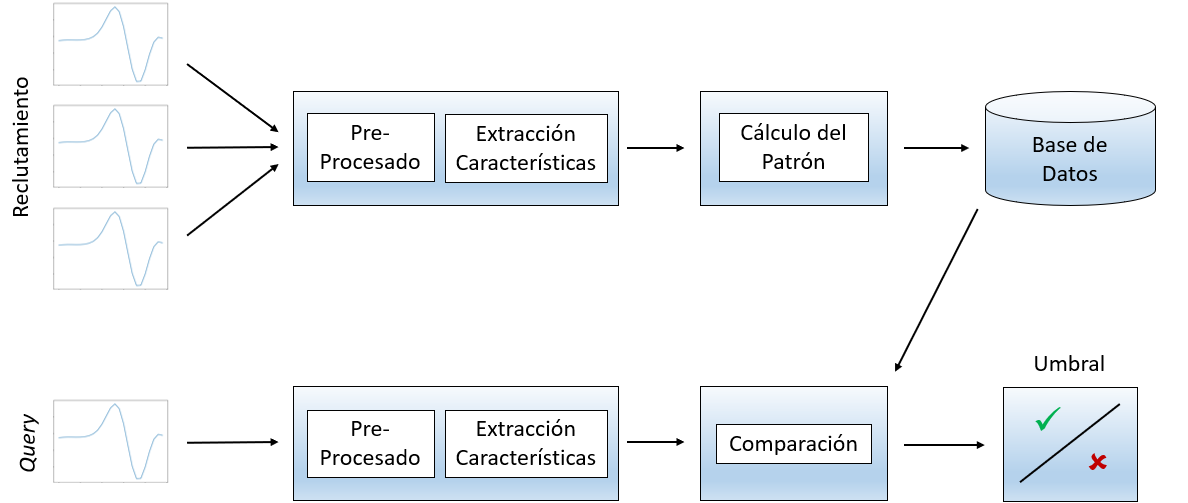
\includegraphics[width=1\textwidth]{/fases_2}
	\caption{Bloques en un sistema de reconocimiento biom�trico.}
	\label{fases}
\end{figure}

En cuanto a la elecci�n del umbral en el caso de autenticaci�n, es interesante destacar que si �ste aumenta, el sistema se relaja, permitiendo una mayor probabilidad de accesos de personas no autorizadas (Tasa de Falsa Aceptaci�n, o FAR), mientras que si disminuye, el sistema se vuelve m�s restrictivo, de manera que aumenta la probabilidad de rechazo para personas autorizadas (Tasa de Falso Rechazo, o FRR). Por tanto, su elecci�n depender� del grado de seguridad que requiera cada sistema.

Adem�s, como se ve en la Figura \ref{fases}, cada una de estas fases est� compuesta por diferentes bloques, que permiten caracterizar a la persona a partir de sus rasgos biol�gicos o de comportamiento . Estas fases son: captura de los datos, pre-procesado de los mismos para facilitar su tratamiento, extracci�n de caracter�sticas (bloque en el que se fundamenta la capacidad del sistema de distinguir entre sujetos) y comparaci�n de las caracter�sticas con las previamente almacenadas. Esta comparaci�n puede estar basada en las distintas t�cnicas de reconocimiento de patrones, como por ejemplo, t�cnicas basadas en modelado de problemas, como las redes neuronales. 
%�AMPLIAR M�S ESTE APARTADO?

%\cite{reillo}
%(en el trabajo de raul lo pone del rev�s, cu�l est� bien�?) 

%Por otro lado, el modo en el que se hace el reclutamiento no es tampoco trivial. En algunas t�cnicas basta una �nica toma de los datos, mientras que en otras puede ser necesario tomar varias muestras y en distintas sesiones (d�as o semanas). A todo esto habr� que a�adir que si el reclutamiento resulta muy pesado, los usuarios del sistema tender�n a rechazar el sistema, por lo que habr� que buscar una soluci�n de compromiso entre la comodidad del usuario, y la obtenci�n de un patr�n �ptimo.
%\newpage

\subsection{Identificaci�n y autenticaci�n} \label{idvsau}
Hasta el momento se ha hecho referencia al reconocimiento biom�trico como algo gen�rico. Sin embargo, cabe diferenciar entre identificaci�n y autenticaci�n. 
\begin{itemize}
	\item Identificaci�n: consiste en determinar la identidad de un usuario registrado en el sistema. Para ello, se comparan las caracter�sticas extra�das con los patrones de todos los usuarios. El principal inconveniente de esta funcionalidad es la necesidad de una base de datos para los patrones, lo que implica una capacidad de almacenamiento elevada y una seguridad apropiada en la custodia de los datos. Como posibles aplicaciones podemos encontrar la identificaci�n de delincuentes a partir de im�genes de videovigilancia o el reconocimiento forense. 
	\item Autenticaci�n o verificaci�n: consiste en determinar si el usuario es realmente quien dice ser. Para ello, adem�s de las caracter�sticas del usuario, �ste tiene que comunicar su identidad. El sistema compara estas caracter�sticas con el patr�n del usuario indicado, que puede estar almacenado en una base de datos o en un sistema port�til de informaci�n, y decide si la petici�n es v�lida o no. Por ejemplo, presentar el pasaporte en una frontera es una aplicaci�n de autenticaci�n de usuarios. 
\end{itemize}

%�Es muy repetitivo?
%La identificaci�n y la autenticaci�n biom�tricas a menudo se llevan a cabo mediante comparaci�n de plantillas o \textit{template matching}. M�s espec�ficamente, una \textit{plantilla biom�trica} es una instancia registrada de las caracter�sticas biom�tricas recogidas durante el reclutamiento del sujeto en el sistema. Esta plantilla es almacenado en una galer�a de plantillas. Cuando se realiza una consulta, se registra una nueva muestra en el sistema y se compara con las plantillas espec�ficas de la identidad solicitada (en autenticaci�n) o con todas las plantillas registradas (en identificaci�n).\cite{samarin}

En este trabajo se va a dise�ar tanto un sistema para la  identificaci�n biom�trica como uno para la autenticaci�n.

\section{Fisiolog�a del coraz�n} \label{fisio}
Antes de analizar la utilidad del electrocardiograma como modalidad biom�trica, esta secci�n presenta un resumen de la fisiolog�a del coraz�n. 

%Aunque el uso del electrocardiograma (ECG) como se�al para el reconocimiento biom�trico es una tendencia que se encuentra todav�a en un estado muy inmaduro, su uso con prop�sitos m�dicos s� ha sido muy extenso en las �ltimas d�cadas, en especial en la detecci�n de patolog�as card�acas y monitorizaci�n de pacientes.
%\begin{figure}[H]
%	\centering
%	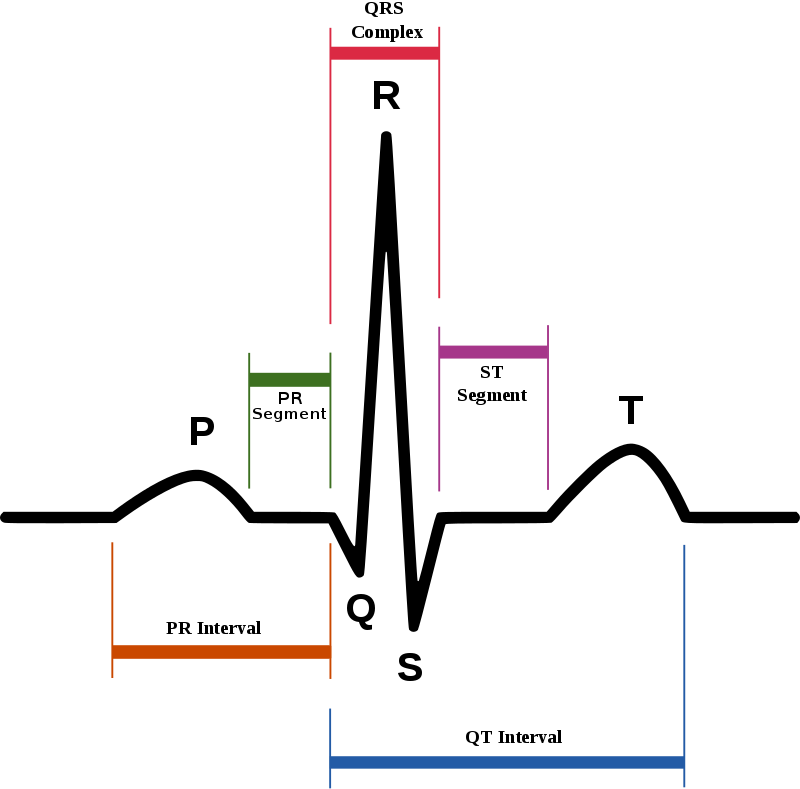
\includegraphics[width=0.5\textwidth]{/ECG}
%	\caption{Esquema General de una se�al de ECG}
%	\label{ondas}
%\end{figure}

El coraz�n es el m�sculo que bombea la sangre en nuestro cuerpo y para ello, se contrae gracias a impulsos el�ctricos. Estos impulsos el�ctricos pueden ser detectados en la superficie del cuerpo mediante el uso de electrodos. As�, el ECG es la representaci�n gr�fica de la actividad el�ctrica del coraz�n, como una se�al en funci�n del tiempo, dando como resultado una curva que representa cada ciclo card�aco y que de forma te�rica se puede ver en la Figura \ref{ondas}. 
Habitualmente, en electrocardiograf�a se utilizan 12 derivaciones para su obtenci�n.


\begin{figure}[H]
	\centering
	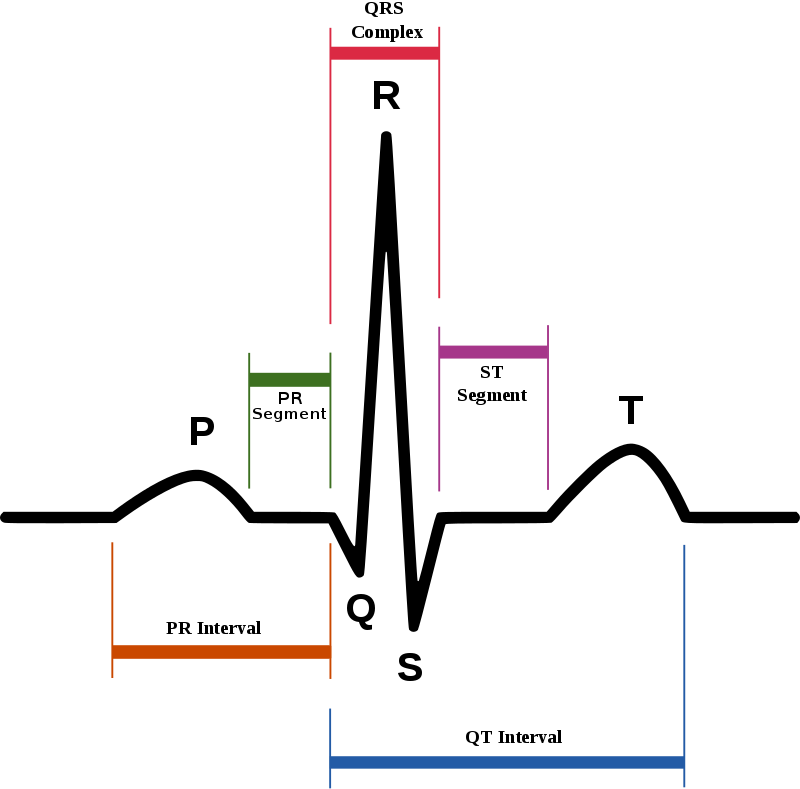
\includegraphics[width=0.55\textwidth]{/ECG}
	\caption{Esquema General de una se�al de ECG. Fuente \cite{samarin}.}
	\label{ondas}
\end{figure}



Como se puede comprobar, dicha se�al se compone de varias partes diferenciadas, que corresponden a la despolarizaci�n y repolarizaci�n de las c�maras del coraz�n, provocando la contracci�n y relajaci�n de las mismas. Las distintas fases del funcionamiento del coraz�n son: 

\begin{itemize}
	\item Onda P: representa la despolarizaci�n de las aur�culas.
	\item Segmento PR: es el tiempo entre la despolarizaci�n de la aur�cula y el inicio de la despolarizaci�n de los ventr�culos.
	\item Complejo QRS: representa la despolarizaci�n de los ventr�culos. Es la parte m�s caracter�stica de la se�al del ECG.
	\item Segmento ST: corresponde al tiempo antes de que los ventr�culos se vuelvan a polarizar.
	\item Onda T: representa la repolarizaci�n ventricular.
	
\end{itemize}

Cada uno de estos componentes podr�a variar tanto en amplitud como en duraci�n, atendiendo a la derivaci�n que se est� tomando, el ritmo card�aco, el estado de estr�s, la posici�n del cuerpo, etc. Evidentemente tambi�n var�an cuando el usuario sufre alguna patolog�a card�aca, tal como arritmias, reflujo ventricular, etc. Todas estas variaciones, adem�s de las propias del sujeto, hacen que utilizar esta informaci�n como modalidad biom�trica, resulte un reto considerable \cite{reillo}.

\section{ECG como modalidad biom�trica}

Tras analizar brevemente la fisiolog�a del coraz�n, en esta secci�n pasamos a considerar si el ECG podr�a ser un elemento biom�trico viable. 

Como ya se ha mencionado en la secci�n \ref{biometria}, para que un sistema biom�trico sea v�lido debe ser universal, �nico y estable, entre otros aspectos. 

En cuanto a la universalidad, es evidente que se cumple en el caso del ECG, pues la actividad el�ctrica del coraz�n est� presente en todos los seres vivos, siendo la falta de esta actividad incompatible con la vida.

Por otro lado, la validaci�n de la unicidad del ECG para su uso como m�todo biom�trico no es tan f�cil de demostrar, debido principalmente a la falta de datos y de estudios que lo prueben. La mayor�a de los trabajos que exploran el uso ECG para la identificaci�n de personas no eval�an el rendimiento del sistema para grandes bases de datos, como se ha hecho en otras modalidades biom�tricas.

Una excepci�n notable es un estudio de Carreiras \textit{et al.} \cite{Carreiras2016}, que se centra en la unicidad de las se�ales de ECG . Los autores de este art�culo cient�fico evaluaron el rendimiento de su sistema biom�trico con una base de datos de registros de ECG recogidos de 618 sujetos y obtuvieron altas tasas de reconocimiento.

Autores como Sufi \textit{et al.}\cite{Sufi2010} afirman la unicidad de la composici�n, el mecanismo y la actividad el�ctrica del coraz�n humano 
bas�ndose en el dogma central de la Biolog�a molecular, que establece que la informaci�n fluye desde el ADN al ARN y de este a las prote�nas.

En el caso de la estabilidad del ECG nos encontramos con todav�a menos estudios que la investiguen. Si bien, es posible demostrar la unicidad utilizando datos registrados en un �nico momento temporal, para demostrar la estabilidad es necesario reunir datos del mismo individuo durante un per�odo de tiempo lo suficientemente largo. La creaci�n de estas grandes bases de datos, para estos estudios longitudinales, es costosa e implica una importante inversi�n de tiempo, lo que explica el reducido n�mero de estudios que examinan la estabilidad del ECG. 

En un estudio de Silva \textit{et al.} \cite{DaSilva2013} se recogieron datos de ECG de 63 sujetos, con dos sesiones de adquisici�n de datos separadas por un intervalo de 4 meses. Sus resultados indican que aunque la autenticaci�n biom�trica funciona peor para los datos de ECG longitudinales, siguen siendo viables para aplicaciones en el mundo real.
 
 
En resumen, el ECG sigue siendo un fuerte candidato a ser usado para el reconocimiento biom�trico. Varios estudios han demostrado la unicidad y la estabilidad del ECG, aunque a peque�a escala. Adem�s, la aparici�n de sensores de ECG de bajo costo proporcionar�a una buena oportunidad para que estos fueran incorporados en los sistemas de control de acceso existentes. En contraposici�n, todav�a no hay suficiente investigaci�n sobre la extracci�n de caracter�sticas de las se�ales del ECG, que permitan prevenir los ataques de falsificaci�n y garantizar que los sistemas biom�tricos basados en ECG sean aceptados por el p�blico en general \cite{samarin}.
 
 
 
 
% Por lo tanto, se puede inferir que la singularidad que proporcionan las entidades biom�tricas existentes se hereda de la singularidad del ADN.
% 
% La composici�n, el mecanismo y la actividad el�ctrica del coraz�n humano heredan la singularidad de la individualidad del ADN.
% 
% En t�rminos biol�gicos, el "dogma central" se refiere al concepto b�sico de que, en la naturaleza, la informaci�n gen�tica fluye generalmente del ADN al ARN (�cido ribonucleico) y a la prote�na.
 
%En uno hablan de que es �nico por el ADN, el otro hace un estudio de la unicidad expl�citamente sobre 600 y pico pacientes. 

%Hablar de la estabilidad. 
%
%�Fases aqu� o las dejo en biometr�a?
%�Algo m�s o pasar ya a objetivos?


\section{Objetivos}

El objetivo principal de este trabajo consiste en el dise�o, desarrollo y evaluaci�n de un novedoso sistema de reconocimiento biom�trico a trav�s del ECG basado en \textit{Deep Learning}. Con este sistema se consigue un avance en el uso de esta modalidad biom�trica interna de las personas, caracter�stica que no solo hace que sea dif�cil de copiar, sino que tambi�n sirve como indicador de vida en la detecci�n de ataques. 
%LO ESTOY PRESENTANDO YO???? 

Como se puede ver en el siguiente cap�tulo (\ref{arte}), esta modalidad cuenta todav�a con muy pocos estudios concluyentes, situ�ndola en un estado muy preliminar. Por ello, este estudio pretende contribuir a la superaci�n de algunas de las limitaciones de las investigaciones existentes, relacionadas con el uso de esta se�al, para el reconocimiento biom�trico.

Para ello, hemos dise�ado y desarrollado un sistema basado en el uso de una red neuronal convolucional, con la que se puede llevar a cabo una extracci�n de caracter�sticas que permite la identificaci�n de un conjunto cerrado (\textit{closed set}) y la autenticaci�n de usuarios. Adem�s, la evaluaci�n de este sistema se ha realizado con se�ales de ECG registradas en varias sesiones, incluyendo tomas despu�s de que el sujeto haya realizado ejercicio, probando que el ECG puede utilizarse caracter�stica biom�trica.

El desarrollo de este proyecto se ha basado en los algoritmos propuestos por Labati \textit{et al.} en el art�culo cient�fico \textit{Deep ECG: Convolutional Neural Networks for ECG biometric recognition} \cite{deepecg}. 




En el capitulo \ref{chap:estado} de este estudio, se revisan las contribuciones  m�s importantes en el �mbito del reconocimiento biom�trico basado en el ECG existentes hasta el momento. Posteriormente, en el cap�tulo \ref{chap:desarrollo} se realiza una descripci�n detallada del desarrollo del sistema propuesto, empezando por una contextualizaci�n del problema y una descripci�n de la base de datos utilizada, y describiendo a continuaci�n, en profundidad, los procesos de preprocesado de la se�al y de extracci�n de caracter�sticas que se han llevado a cabo. En el cap�tulo \ref{chap:resultados} se expone una extensa evaluaci�n del sistema, tanto para la identificaci�n de usuarios como para la verificaci�n de la identidad. Y finalmente, este proyecto concluye en el cap�tulo \ref{chap:conclusiones}, donde adem�s se presentan posibles l�neas futuras de trabajo. 




%%%%%%%%%%%%%%%%%%%%%%%%%%%%%%%%%%%%%%%%%%%%%%%%%%%%%%%%%%%%%%%%%%%%%%%%%%%%%%%!
%
% -- EstadoArte.tex --
%    Estado del arte
%
%%%%%%%%%%%%%%%%%%%%%%%%%%%%%%%%%%%%%%%%%%%%%%%%%%%%%%%%%%%%%%%%%%%%%%%%%%%%%%%!
%!TEX root = ../../Principal/TFG.tex
\chapter{Estado del arte} \label{arte}
\label{chap:estado}
\pagestyle{fancy}
\thispagestyle{empty}
%
\graphicspath{{../EstadoArte/Imagenes/}}
\DeclareGraphicsExtensions{.pdf,.jpg,.png}
%
% Empieza a escribir aqu�


Si bien el uso del ECG como modalidad biom�trica no es una idea nueva, siendo pioneros en esta t�cnica trabajos como el de Biel \textit{et al.} \cite{biel2001} y el de Kyoso \textit{et al.} \cite{Kyoso2001} (2001), esta modalidad todav�a se encuentra en un estado muy inmaduro, no tanto debido al n�mero de estudios existentes, sino a la falta casi absoluta de consenso en las metodolog�as apropiadas para su aplicaci�n. 

Odinaka \textit{et al.} presenta en \cite{Odinaka2012} una extensa y detallada comparativa del estado de la t�cnica hasta el a�o 2012. En este cap�tulo se ofrece una breve descripci�n de la literatura cient�fica de los �ltimos a�os sobre esta modalidad.

A la hora de dise�ar un sistema biom�trico basado en el ECG, hay que tener muy en cuenta una serie de aspectos que van a influir notablemente en su rendimiento. Por esta raz�n, el estado de la t�cnica puede diferenciarse en funci�n de c�mo se han llevado a cabo las etapas de adquisici�n de datos, procesamiento de la se�al y comparaci�n de caracter�sticas.

%\nameref{datos}, el \nameref{procesa} y la \nameref{ext}.
 


\section{Adquisici�n de datos} \label{datos}

La mayor�a de t�cnicas actuales utilizan bases de datos ya existentes y solo unas pocas investigan la estabilidad y usabilidad del ECG como m�todo biom�trico.
 
Si nos fijamos en la posici�n de los electrodos, mientras que la mayor�a de estudios utilizan bases de datos capturadas con electrodos localizados directamente en el cuerpo de la persona \cite{Carreiras2016,Eduardo2017,steven,Jekova2018}, en biometr�a basada en ECG un escenario m�s realista es aqu�l en el que la adquisici�n se realiza con sensores de ECG m�viles. Por ejemplo, Falconi \textit{et al.} \cite{Falconi} incluy� sensores en fundas de smartphones y Silva \textit{et al.} \cite{DaSilva2013} en reposamu�ecas de ordenador. 

Por otro lado, si nos atenemos al tipo de autenticaci�n requerida por el sistema, �sta suele ser una verificaci�n �nica en un instante dado, es decir, en el momento en el que se realiza la petici�n del recurso (para acceder a un edificio o a un servicio bancario, por ejemplo). Sin embargo, tambi�n puede  resultar interesante una autenticaci�n continua, en la que la identidad del usuario se verifica en todo momento mientras el recurso est� en uso (conduciendo un coche, por ejemplo) \cite{deepecg,Pinto2017,Coutinho2011}.

Otro factor a tener en cuenta a la hora de la adqusici�n de las muestras de ECG, es el periodo de tiempo en las que �stas han sido registradas. As�, la estabilidad de los estudios basados en registros tomados en una �nica sesi�n, no pueden considerarse como concluyente. Samarin \textit{et al.} \cite{samarin} aborda esta limitaci�n, teniendo como componente central la confecci�n de una base de datos de ECG propia para la autenticaci�n de usuarios, con dos sesiones diferentes para la toma de datos. Re�llo \textit{et al.} \cite{reillo} tambi�n basa su trabajo sobre una base de datos propia, con una representatividad aceptable tanto para la autenticaci�n intra-clase, como para la inter-clase, registrando muestras en dos d�as diferentes de 105 usuarios.

Por �ltimo, la mayor�a de bases de datos ya existentes tienen un prop�sito m�dico, y no de reconocimiento de usuarios. Esto supone una gran limitaci�n a la hora de usarlas para identificaci�n de personas, pues no son representativas para una realidad en la que la mayor�a de usuarios del sistema biom�trico no tendr�an afecciones card�acas. 

\section{Procesamiento de la se�al} \label{procesa}

La elecci�n de caracter�sticas utilizadas para el procesamiento de la se�al de ECG tambi�n deja clara una falta absoluta de l�nea directriz com�n en las investigaciones existentes. 

El procesamiento de la se�al puede estar basado en el uso de caracter�sticas locales (fiduciales), parcialmente fiduciales o caracter�sticas globales (no-fiduciales). 


Los m�todos fiduciales son aquellos que se basan en obtener, para cada ciclo card�aco, los puntos caracter�sticos (por ejemplo, m�ximo de la onda P, puntos Q, R, S, etc), y obtener de ellos los vectores de caracter�sticas (que constituyen los \textit{templates} o patrones). Estos m�todos se han utilizado con �xito en varios estudios \cite{steven, Jekova2018, Falconi}, pero requieren algoritmos espec�ficos para localizar los puntos de referencia de la se�al.

Los m�todos parcialmente fiduciales localizan s�lo los picos R (en el complejo QRS), y a partir de ellos se segmentan los ciclos card�acos de la se�al. Tras el preprocesado, estos segmentos son adoptados por el sistema biom�trico como patrones \cite{Carreiras2016, DaSilva2013, deepecg}.

Por �ltimo, los m�todos basados en las caracter�sticas globales utilizan mecanismos de procesado tales como la transformada discreta del coseno (DCT), wavelets, redes neuronales, etc. En casi todos estos casos, se parte de la premisa de que un ciclo card�aco va a ser pr�cticamente igual al anterior y al siguiente y no es necesario extraer puntos de referencia de la se�al \cite{Pinto2017,Coutinho2011}. 


\section{Comparaci�n de patrones}\label{ext}

\textit{Template matching}, o comparaci�n de patrones, hace referencia al proceso de verificaci�n de la consulta biom�trica con respecto a los patrones almacenados. Igual que pasa con el procesado, para la comparaci�n de patrones tampoco se puede ver una trayectoria �nica a la hora de determinar qu� algoritmos se deben utilizar. 

En \cite{reillo} se presenta una detallada comparaci�n de las diferentes t�cnicas utilizadas, as� como de los resultados obtenidos. 

En este trabajo, resulta de especial inter�s la aplicaci�n del \textit{Deep Learning}, y en concreto, el uso de redes neuronales convolucionales. La literatura existente presenta numerosos estudios basados en este tipo de aprendizaje aplicado a la Biometr�a, especialmente en reconocimiento facial y de iris, e incluso con se�ales unidimensionales como es el caso del reconocimiento por voz. Sin embargo, la aplicaci�n de las CNNs a la se�al del ECG es considerada por muy pocos estudios hasta la fecha, y la mayor�a se  centran en la clasificaci�n de arritmias y no en aplicaciones biom�tricas \cite{Li2018, Pyakillya2017}. 

As�, el uso de CNNs para el reconocimiento biom�trico basado en ECG es muy novedoso y cuenta con muy pocos estudios llevados a cabo hasta el momento.

En 2017, Song-Kyoo \textit{et al.} present� un posible marco de trabajo para la aplicaci�n de las CNNs en la autenticaci�n biom�trica con ECG en \cite{framework}.

Tambi�n en 2017, Zhang \textit{et al.} present� en \cite{Zhang2017} un algoritmo basado en CNNs para identificar usuarios, utilizando segmentos aleatorios de sus se�ales ECG sin una gran ingenier�a de extracci�n de caracter�sticas y consiguiendo una independencia respecto a los datos utilizados con una gran capacidad de generalizaci�n. Adem�s, unos meses despu�s, propuso en \cite{Zhang2018} un novedoso sistema de ECG corporal, con electrodos colocados en el brazo o detr�s de las orejas, para identificar individuos utilizando estos registros d�biles de los latidos del coraz�n gracias a la aplicaci�n de una red neuronal convolucional, obteniendo resultados prometedores para las ``aplicaciones de salud inteligentes'' (del ingl�s \textit{smart health applications}). 


%Zhang 1 = 93,5% !!!
%zhang 2 =  98.4% (single-arm-ECG) and 91.1% (ear-ECG)

 
\textit{Deep-ECG: Convolutional Neural Networks for ECG biometric recognition} \cite{deepecg}, publicado en 2019 y utilizado como estudio de referencia en este trabajo, utiliza las CNNs para extraer caracter�sticas de usuarios durante la fase de entrenamiento de la red y a continuaci�n realiza una fase de identificaci�n \textit{closed set}, y otra de verificaci�n de la identidad y re-autenticaci�n peri�dica, con usuarios diferentes a los utilizados para entrenar la red. 

Y finalmente, tambi�n en 2019, Pinto \textit{et al.} present� otras dos aplicaciones de las CNNs para el reconocimiento biom�trico basado en ECG en \cite{Pinto2019} y \cite{deep}. Ambos estudios presentan novedosos m�todos que permiten llevar a cabo tanto la identificaci�n como la autenticaci�n de usuarios sin la necesidad de preprocesar las se�ales ECG, obteniendo resultados muy prometedores para ambas modalidades tras una evaluaci�n de los m�todos propuestos sobre varias bases de datos. 

%: \textit{An End-to-End Convolutional Neural Network for ECG-Based Biometric Authentication}\cite{Pinto2019} y \textit{Deep Neural Networks For Biometric Identification Based On Non-Intrusive ECG Acquisitions} \cite{deep}. Ambos estudios presentan novedosos m�todos que permiten llevar a cabo tanto la identificaci�n como la autenticaci�n de usuarios sin la necesidad de preprocesar las se�ales ECG, y han obtenido resultados muy prometedores para ambas modalidades tras una evaluaci�n de los m�todos propuestos sobre varias bases de datos. 





%SE ME HA QUEDADO SIN PONER EL DE CONV 2D

La siguiente Tabla \ref{tablacompa} muestra una comparativa de los resultados obtenidos en estos �ltimos trabajos citados. 




\begin{table}[H]
\centering
%\begin{tabularx}{1\textwidth}{ 
%		%c c c c c c }
%		>{\raggedright\arraybackslash}X
%		>{\centering\arraybackslash}X
%		>{\centering\arraybackslash}X
%		>{\centering\arraybackslash}X
%		>{\centering\arraybackslash}X
%		>{\raggedleft\arraybackslash}X}
 \resizebox{\textwidth}{!}{%
	\begin{tabular}{c c c c c c }
	\hline
	Autor & Usuarios & Preprocesado & M�todo & Tasa de Identificaci�n & EER de autenticaci�n \\
	\hline
	Labati \textit{et al.} \cite{deepecg} & 52 & Parcialmente-local & CNN & 100\% & 1,05 \\
	\hline
	Zhang \textit{et al.} \cite{Zhang2017}& 18 a 47 & Sin preprocesar & CNN & 93,5\% & - \\
	\hline
	Zhang \textit{et al.} \cite{Zhang2018}& 18 a 47 & Parcialmente-local & CNN & 95\% & - \\
	\hline
	Pinto \textit{et al.} \cite{Pinto2019}& 1019 & Sin preprocesar &CNN  & - & 7,86\% \\
	\hline
	Pinto \textit{et al.} \cite{deep}& 1019 & Sin preprocesar & CNN & 96,1\% & - \\
	\hline
	Salloum {et al.} \cite{autentiguia}& 47 &  Parcialmente-local & RNN & 100\% & 0\% \\
	\hline

\end{tabular}}
\caption{Comparativa de estudios existentes basados en redes neuronales para la identificaci�n y autenticaci�n biom�trica a trav�s del ECG.}
\label{tablacompa}
\end{table}


Como conclusi�n, es muy dif�cil poder comparar los resultados obtenidos en los diversos trabajos previos debido a la falta de consenso casi absoluta existente en esta t�cnica biom�trica, lleg�ndonos incluso a encontrar discrepancias sobre qu� m�tricas usar a la hora de evaluar los sistemas dise�ados. Por tanto, el ECG como modalidad biom�trica es una t�cnica novedosa muy prometedora, pero hasta el momento en un estado muy preliminar.


%%%%%%%%%%%%%%%%%%%%%%%%%%%%%%%%%%%%%%%%%%%%%%%%%%%%%%%%%%%%%%%%%%%%%%%%%%%%%%%!
%
% -- Resultados.tex --
%    Resultados y conclusiones
%
%%%%%%%%%%%%%%%%%%%%%%%%%%%%%%%%%%%%%%%%%%%%%%%%%%%%%%%%%%%%%%%%%%%%%%%%%%%%%%%!
%!TEX root = ../../Principal/TFG.tex
\chapter{Desarrollo del sistema propuesto}
\label{chap:desarrollo}
\pagestyle{fancy}
\thispagestyle{empty}
%
\graphicspath{{../Desarrollo/Imagenes/}}
\DeclareGraphicsExtensions{.pdf,.jpg,.png}

%
% Empieza a escribir aqu�
\section{Contexto y planteamiento del problema }

Como ya se ha comentado, este trabajo implementa y eval�a un sistema de reconocimiento biom�trico a trav�s del ECG basado en redes neuronales convolucionales (CNN), con el que se puede realizar tanto la modalidad de identificaci�n de usuarios como la de autenticaci�n. Para ello, el desarrollo se ha basado en los algoritmos propuestos en el art�culo cient�fico \textit{Deep-ECG: Convolutional Neural Networks for ECG biometric recognition} \cite{deepecg}. 

Para ambas modalidades, el novedoso enfoque presentado en \cite{deepecg} que se ha utilizado en este estudio consiste en extraer un conjunto de $m$ complejos QRS de registros de ECG de corta duraci�n y concatenarlos, obteniendo una nueva se�al \textbf{V}. En la identificaci�n \textit{closed set}, una CNN procesa \textbf{V} e indica qui�n es el usuario registrado m�s cercano. En la verificaci�n de la identidad, la CNN procesa \textbf{V} para obtener un patr�n biom�trico \textbf{T} y, mediante la t�cnica de comparaci�n de patrones (o \textit{template matching}), da una respuesta a la autenticaci�n en base a la medida de la distancia eucl�dea.  
%CHECKEAR TEMPLATE!!!!!!
%REPETIR IMAGEN
\begin{figure}[H]
	\centering
	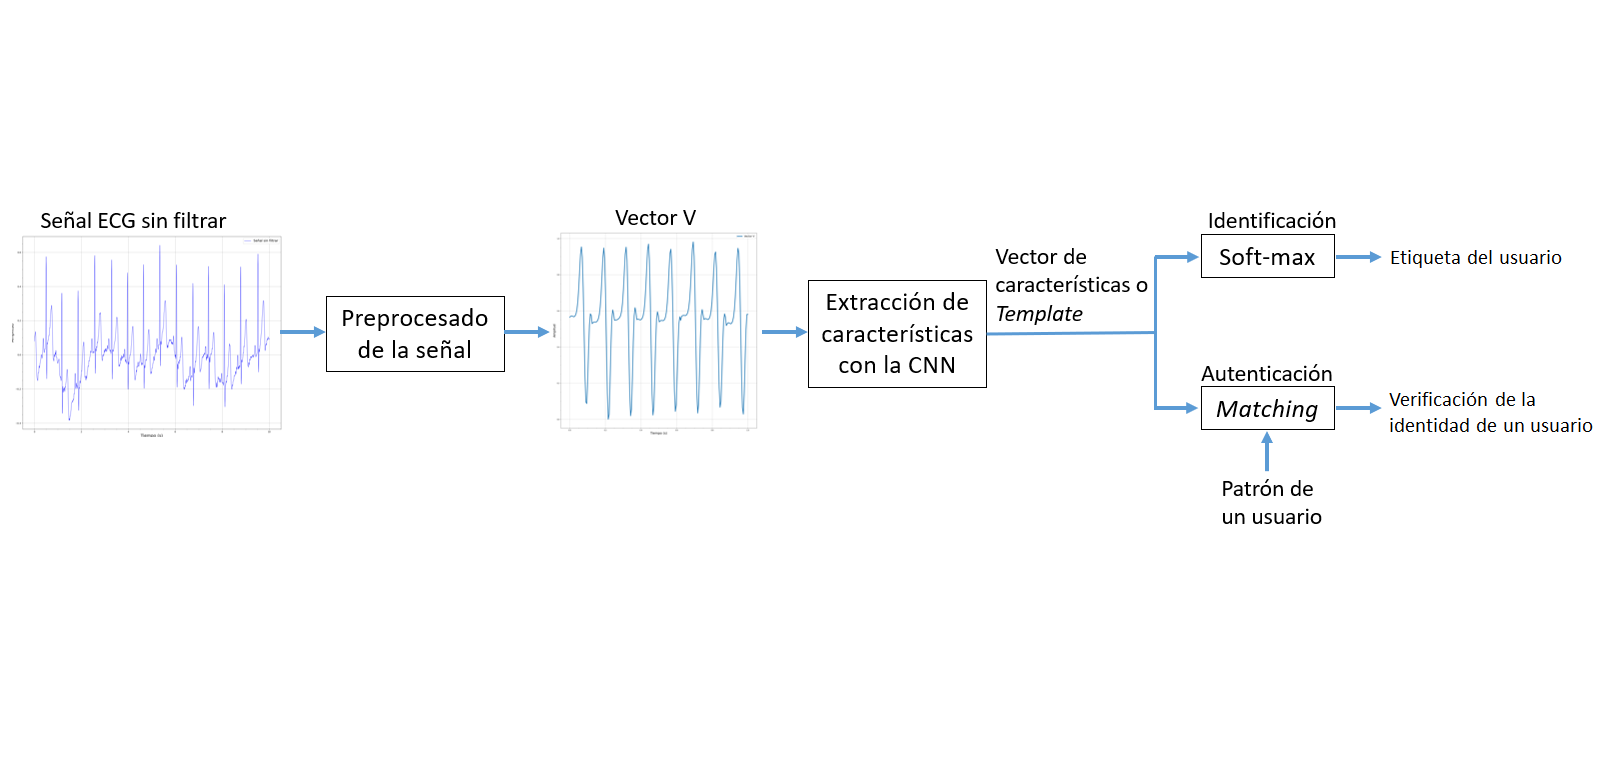
\includegraphics[width=0.9\textwidth]{/pipeline_1}
	\caption{Flujo de Trabajo.}
	\label{pipeline}
\end{figure}

El flujo de trabajo est� dividido en las siguientes etapas (Figura \ref{pipeline}):
\begin{itemize}
	\item Preprocesamiento de la se�al.
	\item Extracci�n de caracter�sticas con la CNN.
	\item Reconocimiento biom�trico.
	\begin{enumerate}
		\item Identificaci�n basada en \textit{Soft-max}.
		\item Autenticaci�n basada en comparaci�n de patrones. 
	\end{enumerate}
\end{itemize}

%A�ADIR ALGO SOBRE DEPORTE Y NO DEPORTE Y ALGO SOBRE OPEN SET IDENTIFICATION?????

Adem�s, con este estudio se ha querido analizar la estabilidad del ECG como caracter�stica biom�trica, utilizando registros de la se�al obtenidos en dos sesiones diferentes y utilizando experimentos diferentes seg�n la toma de datos.

Todo el desarrollo de este proyecto ha sido implementado con el lenguaje de programaci�n Python \cite{python}, que es el lenguaje m�s utilizado hoy en d�a para construir y entrenar redes neuronales y, en particular, redes neuronales convolucionales. La sintaxis de \break Python se caracteriza por su sencillez, que hace que sea f�cil de usar y r�pido de aprender. Adem�s, este lenguaje tiene licencia de c�digo abierto y cuenta con una amplia cantidad de bibliotecas disponibles para el \textit{Deep Learning}, incluyendo NumPy \cite{Oliphant2006}, scikit-learn \cite{skit}, as� como con todas las plataformas m�s populares y poderosas de este campo. 
Una de ellas es Keras \cite{keras}, que se ha utilizado en este proyecto para la implementaci�n de todas las CNNs. Keras es una biblioteca de \textit{Deep Learning} de alto nivel, que se ejecuta t�picamente sobre TensorFlow \cite{tensorflow}. Esta biblioteca permite una r�pida experimentaci�n y se caracteriza por su modularidad y extensibilidad, que permiten  combinar y a�adir capas neuronales, funciones de activaci�n, hiperpar�metros y otros elementos con facilidad.


%los principales marcos de aprendizaje profundo apoyan a Python. De estos, las plataformas m�s populares y poderosas son TensorFlow, Keras (que se utiliza t�picamente como un envoltorio de front-end para TensorFlow), y PyTorch.
% 
%Keras es un marco de aprendizaje profundo de alto nivel que se ejecuta sobre TensorFlow, Microsoft Cognitive Toolkit o Theano (pero en la pr�ctica, m�s com�nmente utilizado con TensorFlow). Keras proporciona convenientes abstracciones de programaci�n que le permiten trabajar con construcciones de aprendizaje profundo como modelos, capas e hiperpar�metros, no con tensores y matrices.
%
%
%Keras [11] es una librer�a enfocada al dise�o de redes neuronales, que se puede ejecutar sobre numerosas plataformas, entre ellas TensorFlow.  
%
%Hay muchos marcos y bibliotecas de Python disponibles para la m�quina y el aprendizaje profundo, incluyendo NumPy, scikit-learn, as� como los "tres grandes" marcos de aprendizaje profundo que discutimos en la siguiente secci�n


 




\section{Base de datos}

%Hablar aqu� de las bases de datos existentes? solo de la m�a? 
 
Como se ha podido ver en el cap�tulo \ref{arte}, no existe un consenso sobre qu� requisitos deben cumplir las bases de datos utilizadas para el dise�o de sistemas biom�tricos basados en ECG, haciendo muy dif�cil una posible comparativa entre m�todos. Las t�cnicas de adquisici�n de datos utilizadas actualmente var�an en par�metros tan importantes como la configuraci�n de los electrodos, el tiempo de adquisici�n, el n�mero de sujetos o el n�mero de sesiones, entre muchos otros. Adem�s, existen diferencias entre si la autenticaci�n es continua o si la verificaci�n de la identidad del usuario es requerida para un instante dado.



%Independientemente de esto, est� claro que en la mayor�a de las bases de datos, se tiene s�lo una muestra continua de cada usuario, por lo que no se pueden extrapolar datos respecto a la repetitividad de los datos en d�as distintos. Por lo tanto, la viabilidad de utilizar estas bases de datos en el trabajo expuesto es pr�cticamente nula, as� como la de validar los resultados ofrecidos por aquellos autores que hayan usado estas bases de datos para su investigaci�n.

Afortunadamente, para la realizaci�n de este trabajo se ha podido contar con una base de datos ya existente y dise�ada especialmente para aplicaciones de identificaci�n y autenticaci�n. 

La captura de las muestras se llev� a cabo utilizando BioPac MP100, un equipo comercial de ECG, y los usuarios participantes fueron 105 personas sanas, con edades comprendidas entre los 19 y los 60 a�os, siendo 54 mujeres y 51 hombres.

Esta base de datos, a su vez puede ser dividida en dos, seg�n el tipo de experimento realizado para la toma de los datos. As�, la captura de los mismos se rige de la siguiente manera:
%datos, datos datos, datos
\begin{itemize}
	\item Para obtener variabilidad intra-clase, se llevaron a cabo 2 sesiones de captura por cada usuario, separadas entre s� un m�nimo de una semana.
	\item Para la \textbf{primera base de datos, constituida por los 50 primeros sujetos}, ambas sesiones son iguales:
	\begin{itemize}
		\item En la primera toma, el usuario se encuentra sentado, en actitud relajada y con los ojos abiertos.
		\item En la segunda toma, el usuario se encuentra tambi�n sentado y en actitud relajada, pero esta vez con los ojos cerrados. 
	\end{itemize}

	\item Para la \textbf{segunda base de datos, constituida por los siguientes 55 sujetos}, las sesiones var�an:
	
	\begin{itemize}
		\item Para la primera sesi�n:
			\begin{itemize}
				\item La primera toma es igual que para la primera base de datos.
				\item En la segunda toma, el usuario se encuentra de pie, con los ojos abiertos y en actitud relajada.
			\end{itemize}
		\item Para la segunda sesi�n:
			\begin{itemize}
				\item La primera toma se mantiene.
				\item En la segunda toma, el usuario est� sentado, y se realiza despu�s de haberse ejercitado en un \textit{stepper} durante 5 minutos hasta llegar a los 130 latidos por minuto.
			\end{itemize}
	\end{itemize}
	\item Cada toma de datos se repiti� 5 veces y cada una tiene una duraci�n de 60 segundos. Cada usuario tiene 20 tomas.
	\item La se�al ECG fue capturada en las mu�ecas de los usuarios.
	\item La frecuencia de muestreo se fij� a 1 KHz.
	\item Adem�s, como la base de datos completa la forman 105 usuarios, se consigui� una representatividad aceptable de la distribuci�n inter-clase.
\end{itemize}

La Figura \ref{qrss} muestra visualmente las posibles diferencias que existen, para un mismo usuario, entre las dos sesiones de captura, entre estar sentado y de pie, y entre estar en reposo o despu�s de hacer ejercicio. 

\begin{figure}[h!]
	\centering
	\subfigure{
		%\label{fig:heliceuno}
		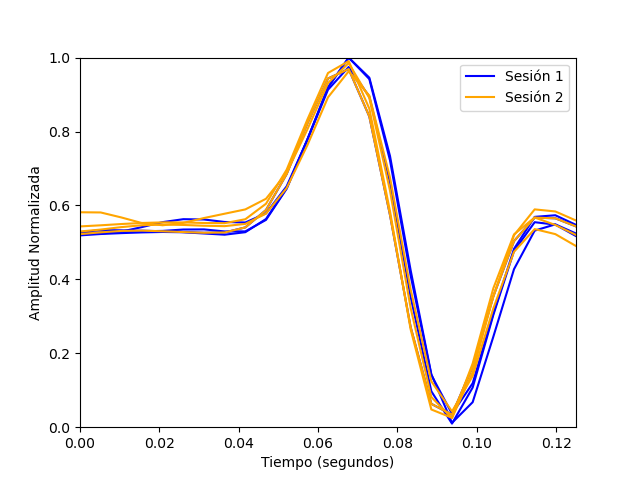
\includegraphics[width=0.3\textwidth]{/qrs_sesiones}}
	\subfigure{
		%\label{fig:ferula}
		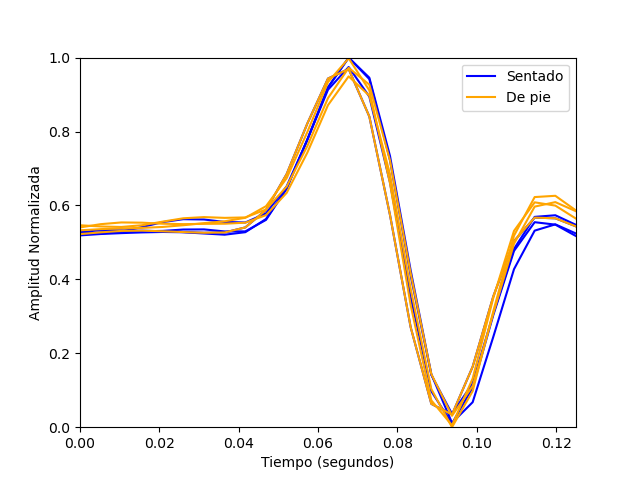
\includegraphics[width=0.3\textwidth]{/qrs_sentadodepie}}
	\subfigure{
		%\label{fig:heliceuno}
		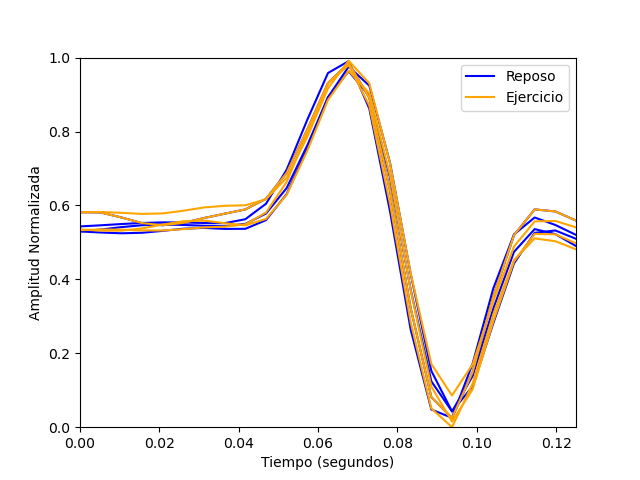
\includegraphics[width=0.3\textwidth]{/qrs_deporte}}
	\caption{Examen visual de la variabilidad entre los casos capturados.}
	\label{qrss}
\end{figure}


Como se puede ver, no existe una gran variabilidad entre la primera sesi�n y la segunda sesi�n. S� que se aprecia una peque�a variaci�n (especialmente en la onda T) entre estar sentado y estar de pie. La variaci�n es algo m�s significativa entre las muestras obtenidas tras haber hecho ejercicio. 




\section{Prepocesado de la se�al de ECG}

En esta secci�n se describe la etapa de preprocesado de las se�ales del ECG, que tiene como objetivo mejorar su calidad y extraer de ellas los complejos QRS m�s discriminantes. Para ello, nos hemos basado en los algoritmos presentados en el art�culo de referencia \cite{deepecg}.

\subsection{Filtrado de la se�al}
Antes de llevar a cabo el filtrado de las se�ales, para obtener las muestras biom�tricas que se van a emplear en el entrenamiento y en la evaluaci�n del sistema, la frecuencia de muestreo de cada toma se ha reducido de 1000 Hz a 200 Hz. Adem�s, cada se�al de 60 segundos se ha dividido en intervalos de 10 segundos, periodo que se utiliza t�picamente para el an�lisis m�dico \cite{deepecg}. Por tanto, para cada usuario ahora hay 120 tomas registradas. 

Realizar un filtrado adecuado para las se�ales del ECG requiere tener en cuenta las componentes de ruido que puedan estar presentes, y las componentes de frecuencia de las diferentes ondas que describe el coraz�n (descritas en la secci�n \ref{fisio}), especialmente del complejo QRS. 

T�picamente, el electrocardiograma tiene dos fuentes de ruido principales \cite{framework,removing,approaches}: 
%EN REALIDAD SON TRES!
\begin{itemize}
	\item Variaciones de baja frecuencia de la l�nea base (o en ingl�s \textit{Baseline Wander}) causadas por el uso de electrodos inapropiados, movimientos del sujeto y la propia respiraci�n. Esto genera un "desplazamiento" de la l�nea base arriba y abajo que se encuentran en el rango de 0,5 Hz, aunque un mayor movimiento del sujeto al realizar ejercicio o pruebas de estr�s pueden aumentar su frecuencia. Para eliminar esta fuente de ruido, bastar�a con aplicar un filtro de respuesta finita al impulso (\textit{FIR}) de paso alto con una frecuencia de corte de 0,5 Hz. 
	\item Interferencias de red, presentes en cualquier se�al bio-el�ctrica registrada desde la superficie del cuerpo de una persona. Este ruido se caracteriza por ser una interferencia sinusoidal de 50-60 Hz, posiblemente acompa�ada de una serie de arm�nicos. Para eliminarlo, puede utilizarse un filtro notch de respuesta infinita al impulso (\textit{IIR}). 
\end{itemize}

Teniendo esto en cuenta, para reducir el ruido global de la se�al del ECG, tambi�n podr�a utilizarse un filtro paso-banda, como puede ser el filtro paso banda de \textit{Butterworth}, que se caracteriza por una respuesta muy uniforme a las frecuencias dentro de la banda de paso \cite{samarin,reillo,deep}. 

%(ESTO AQU� TIENE SENTIDO???)
Respecto a qu� componentes de frecuencia son m�s �tiles para analizar las diferentes ondas presentes en el ECG, no existe un consenso absoluto, y diferentes investigadores muestran distintas respuestas, consider�ndose incluso que el ancho de banda �til para analizar el complejo QRS var�a en funci�n de la persona e incluso en funci�n del tiempo para una misma persona \cite{850hz, hblocks, ult}. 

Con el fin de mejorar la calidad de las se�ales de nuestra base de datos, se han probado los diferentes filtros citados, experimentando con diferentes frecuencias de corte y con distintos valores de orden, y finalmente se ha utilizado un filtro \textit{Butterworth} paso banda entre 1 y 35 Hz de orden 5. El resultado de aplicar este filtro sobre la se�al sin procesar se puede ver en la Figura \ref{filtro}

\begin{figure}[H]
	\centering
	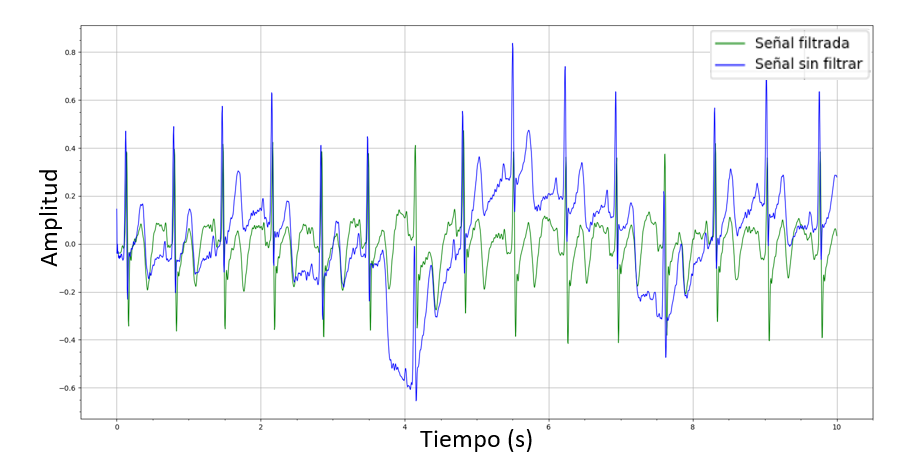
\includegraphics[width=0.8\textwidth]{/filtro}
	\caption{Resultado de aplicar un filtro paso-banda Butterworth.}
	\label{filtro}
\end{figure}

Adem�s, la Figura \ref{espectro}, muestra el espectro en frecuencia de la se�al de ECG antes y despu�s de aplicar el filtro, donde se puede apreciar claramente como se ha eliminado el ruido de baja frecuencia correspondiente a la \textit{Baseline Wander}. El ruido debido a las interferencias de red, sin embargo, solo es apreciable en la escala logar�tmica. 




%REPASAR ESTE P�RRAFO

\begin{figure}[H]
	\centering
	\subfigure[Espectro en frecuencia de la se�al sin filtrar.]{
		\label{fig:esp_sin}
		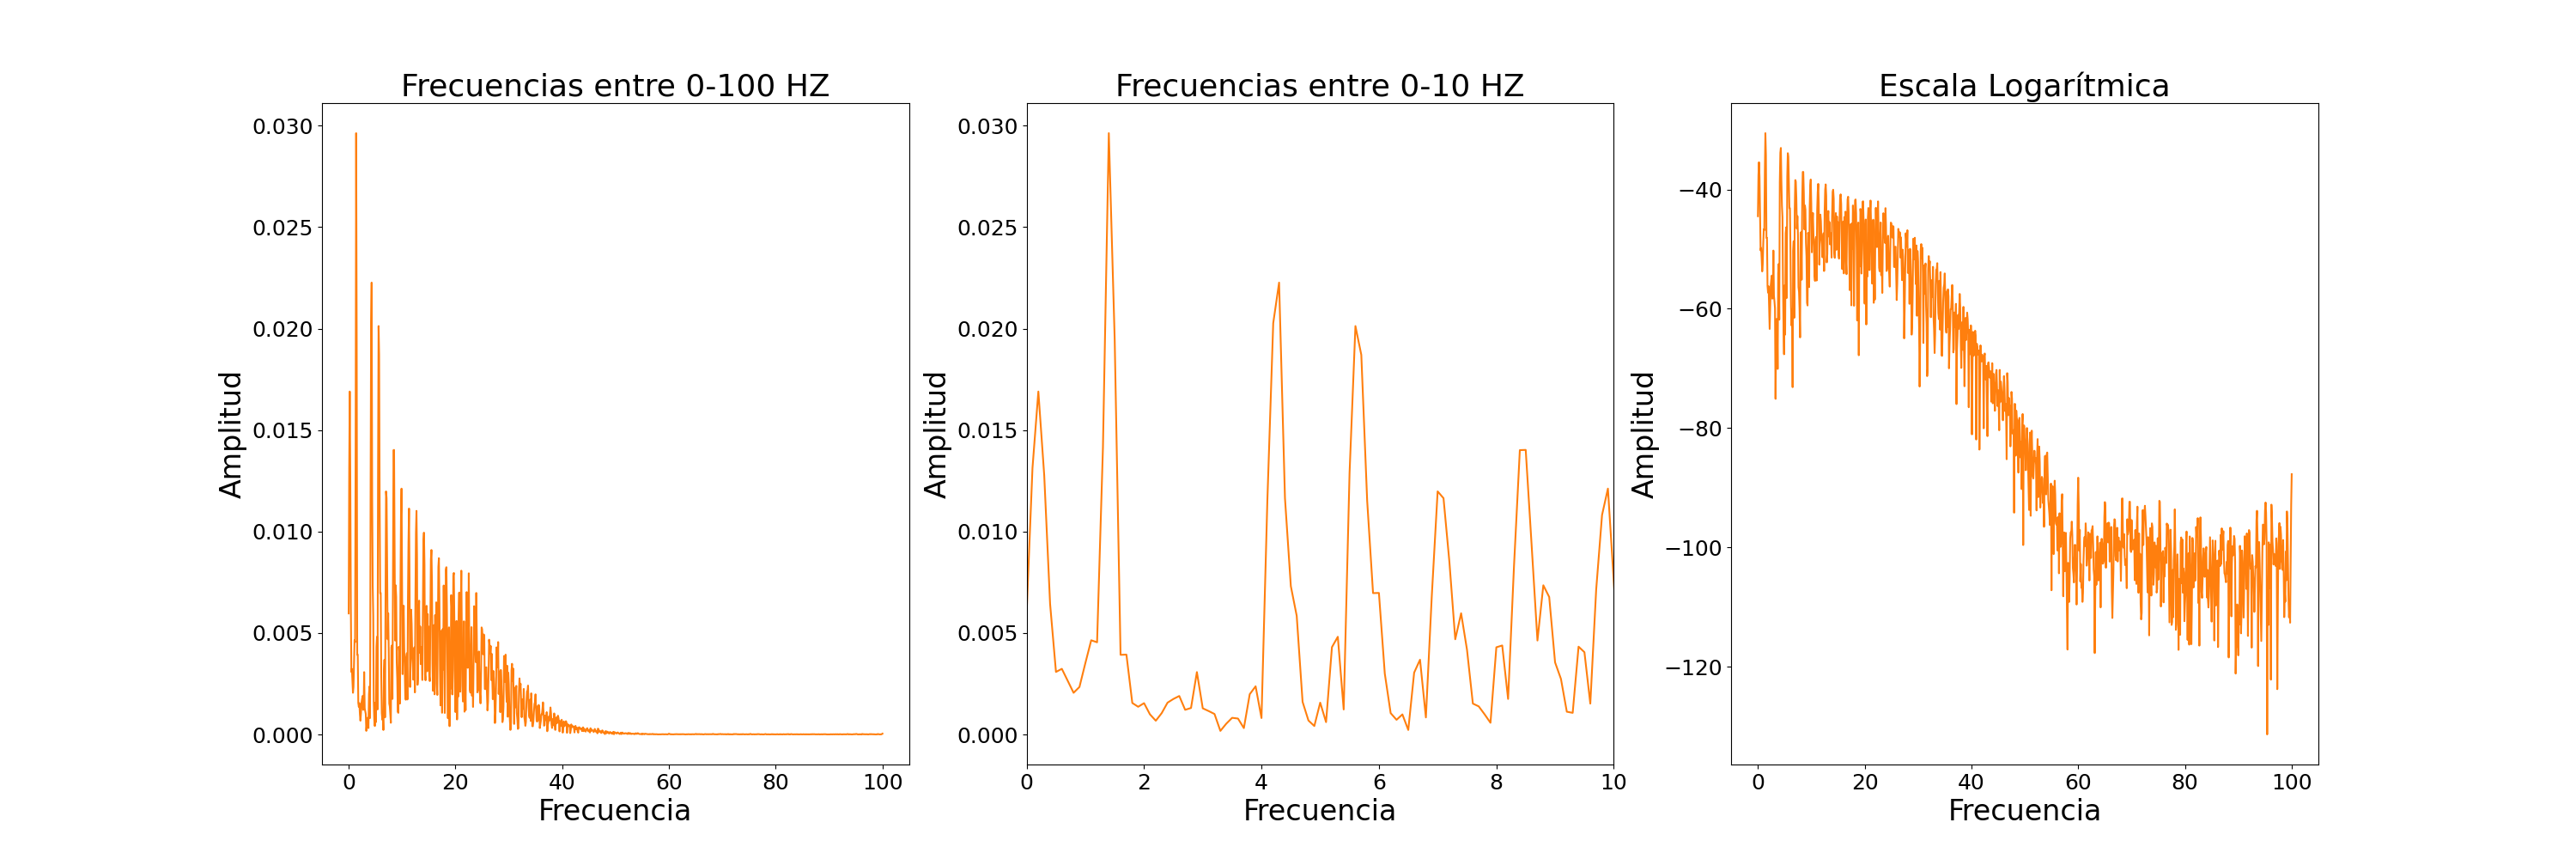
\includegraphics[width=0.8\textwidth]{/espectro_sin}}
	\subfigure[Espectro en frecuencia de la se�al filtrada.]{
		\label{fig:esp_con}
		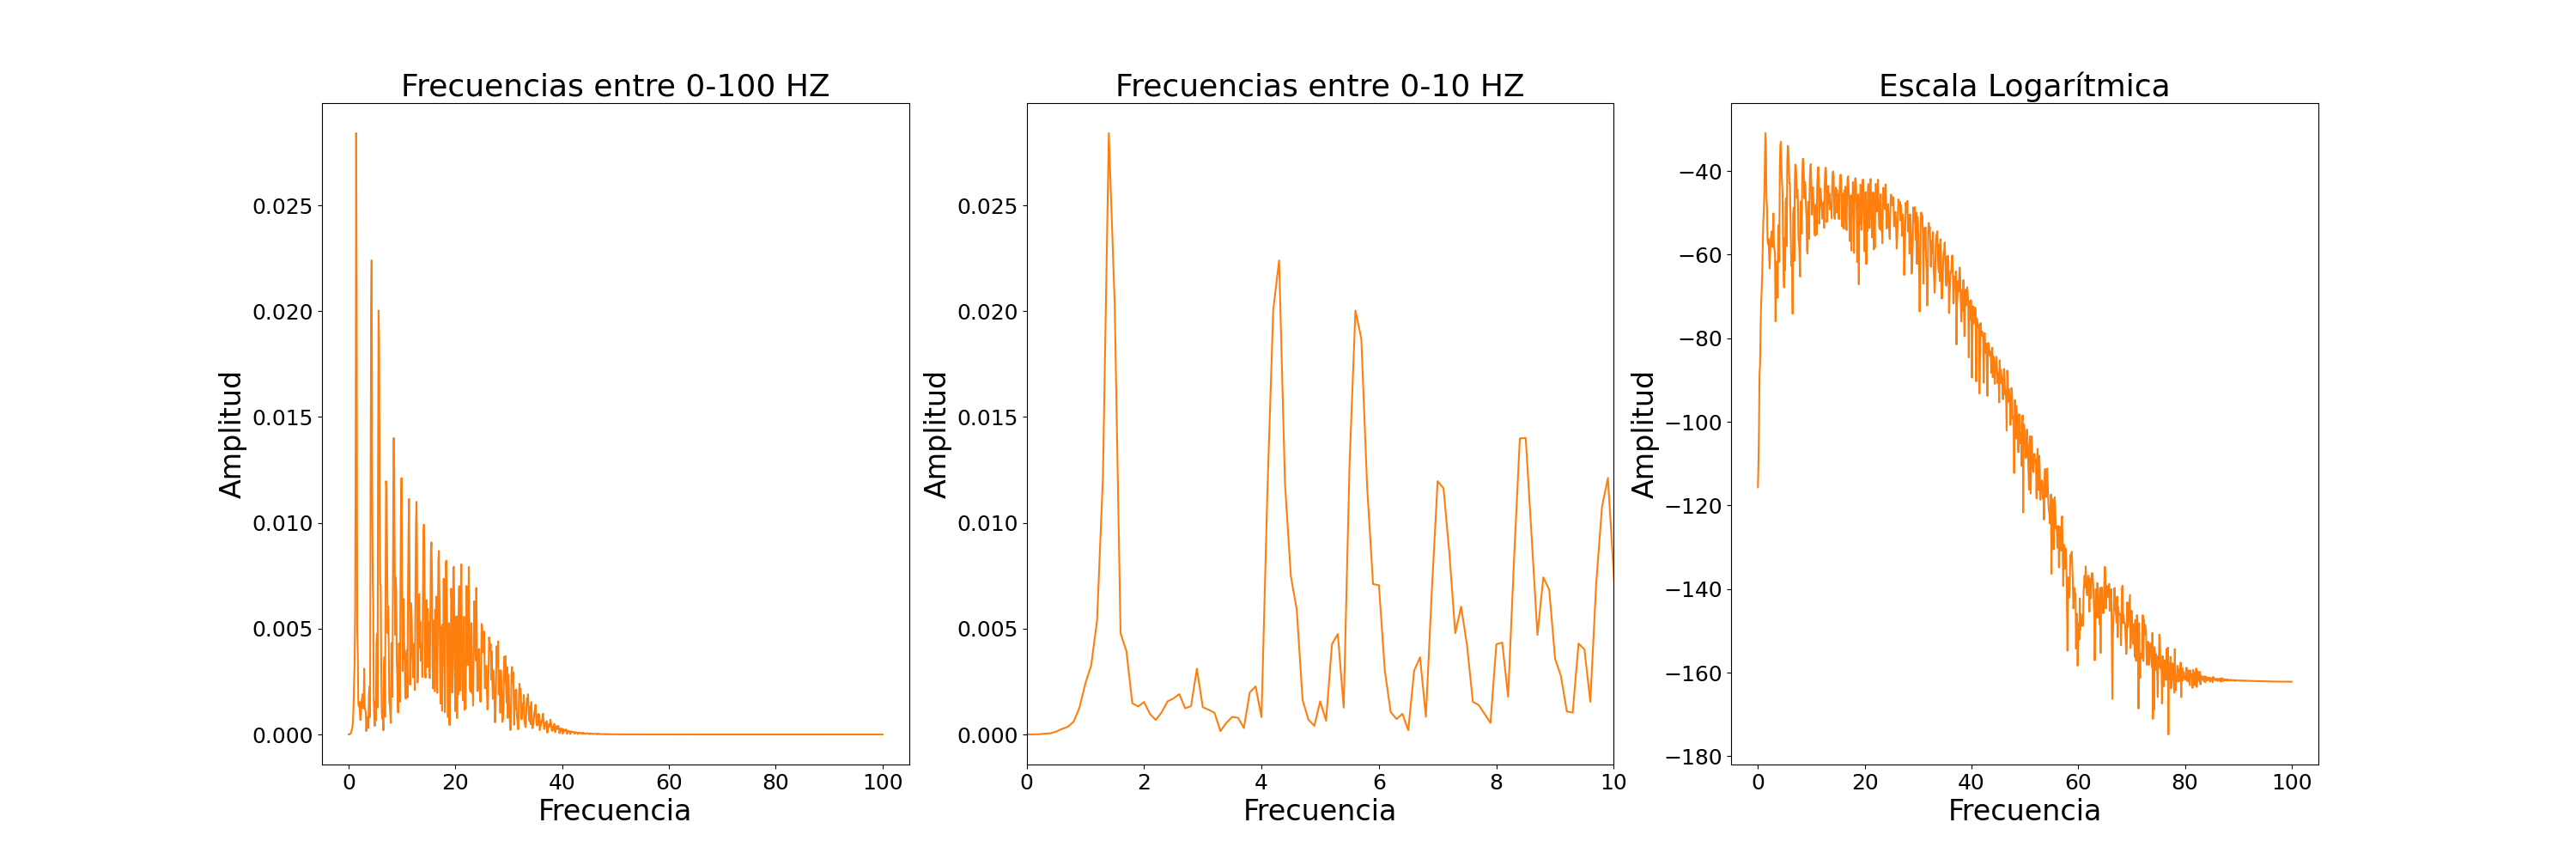
\includegraphics[width=0.8\textwidth]{/espectro_filtro}}
	
	\caption{Espectro en frecuencia de la se�al de ECG antes y despu�s de aplicar un filtro paso-banda Butterworth.}
	\label{espectro}
\end{figure}

Tambi�n se realiz� un filtrado mucho m�s agresivo sobre la se�al, con un filtro \textit{Butterworth} paso banda entre 5 y 20 Hz, como se utiliz� en el estudio realizado por Carreiras \textit{et al.} \cite{Carreiras2016}. Si bien este filtrado permit�a mejorar la precisi�n en la detecci�n de picos R, los resultados obtenidos para la identificaci�n de personas fueron notablemente peores (84\% frente a 97\%). Esto demuestra que la selecci�n de un filtrado adecuado influye de forma significativa en el funcionamiento de la red, y que si se eliminan demasiadas componentes de frecuencia del complejo QRS, la red no es capaz de distinguir entre los diferentes sujetos con tanta precisi�n.

\subsection{Segmentaci�n de la se�al y obtenci�n del vector V}
%Detecci�n de picos, obtenci�n del vector h y obtenci�n del vector V, descarto los problem�ticos
El siguiente paso, una vez mejorada la calidad de la se�al de ECG, es la extracci�n de los complejos QRS. 
%Aqu� o al principio?
El uso de este complejo para  prop�sitos biom�tricos puede ser muy beneficioso, al ser la parte del ECG menos sensible a las variaciones debidas al esfuerzo f�sico o al estado emocional de la persona. 
As�, el QRS puede utilizarse para extraer los rasgos que componen los patrones biom�tricos de cada individuo.

Como se ha explicado anteriormente (cap�tulo \ref{arte}), los sistemas biom�tricos basados en el ECG se pueden clasificar en funci�n de si su procesamiento se basa en el uso de caracter�sticas locales (o sea, fiduciales) o caracter�sticas globales (no-fiduciales). 
%hablar de esto en el estado del arte!!! si no, explicarlo aqu�
En este caso, el enfoque es parcialmente-fiducial, es decir, mediante la localizaci�n de los picos R se extraen las caracter�sticas de las ondas de los latidos del coraz�n, concretamente del complejo QRS. 

Por tanto, el primer paso es la detecci�n del pico R de cada latido. La b�squeda de este punto es generalmente m�s sencilla que la b�squeda de otros puntos de referencia, porque es el pico m�s alto y m�s agudo en un latido.

\begin{figure}[H]
	\centering
	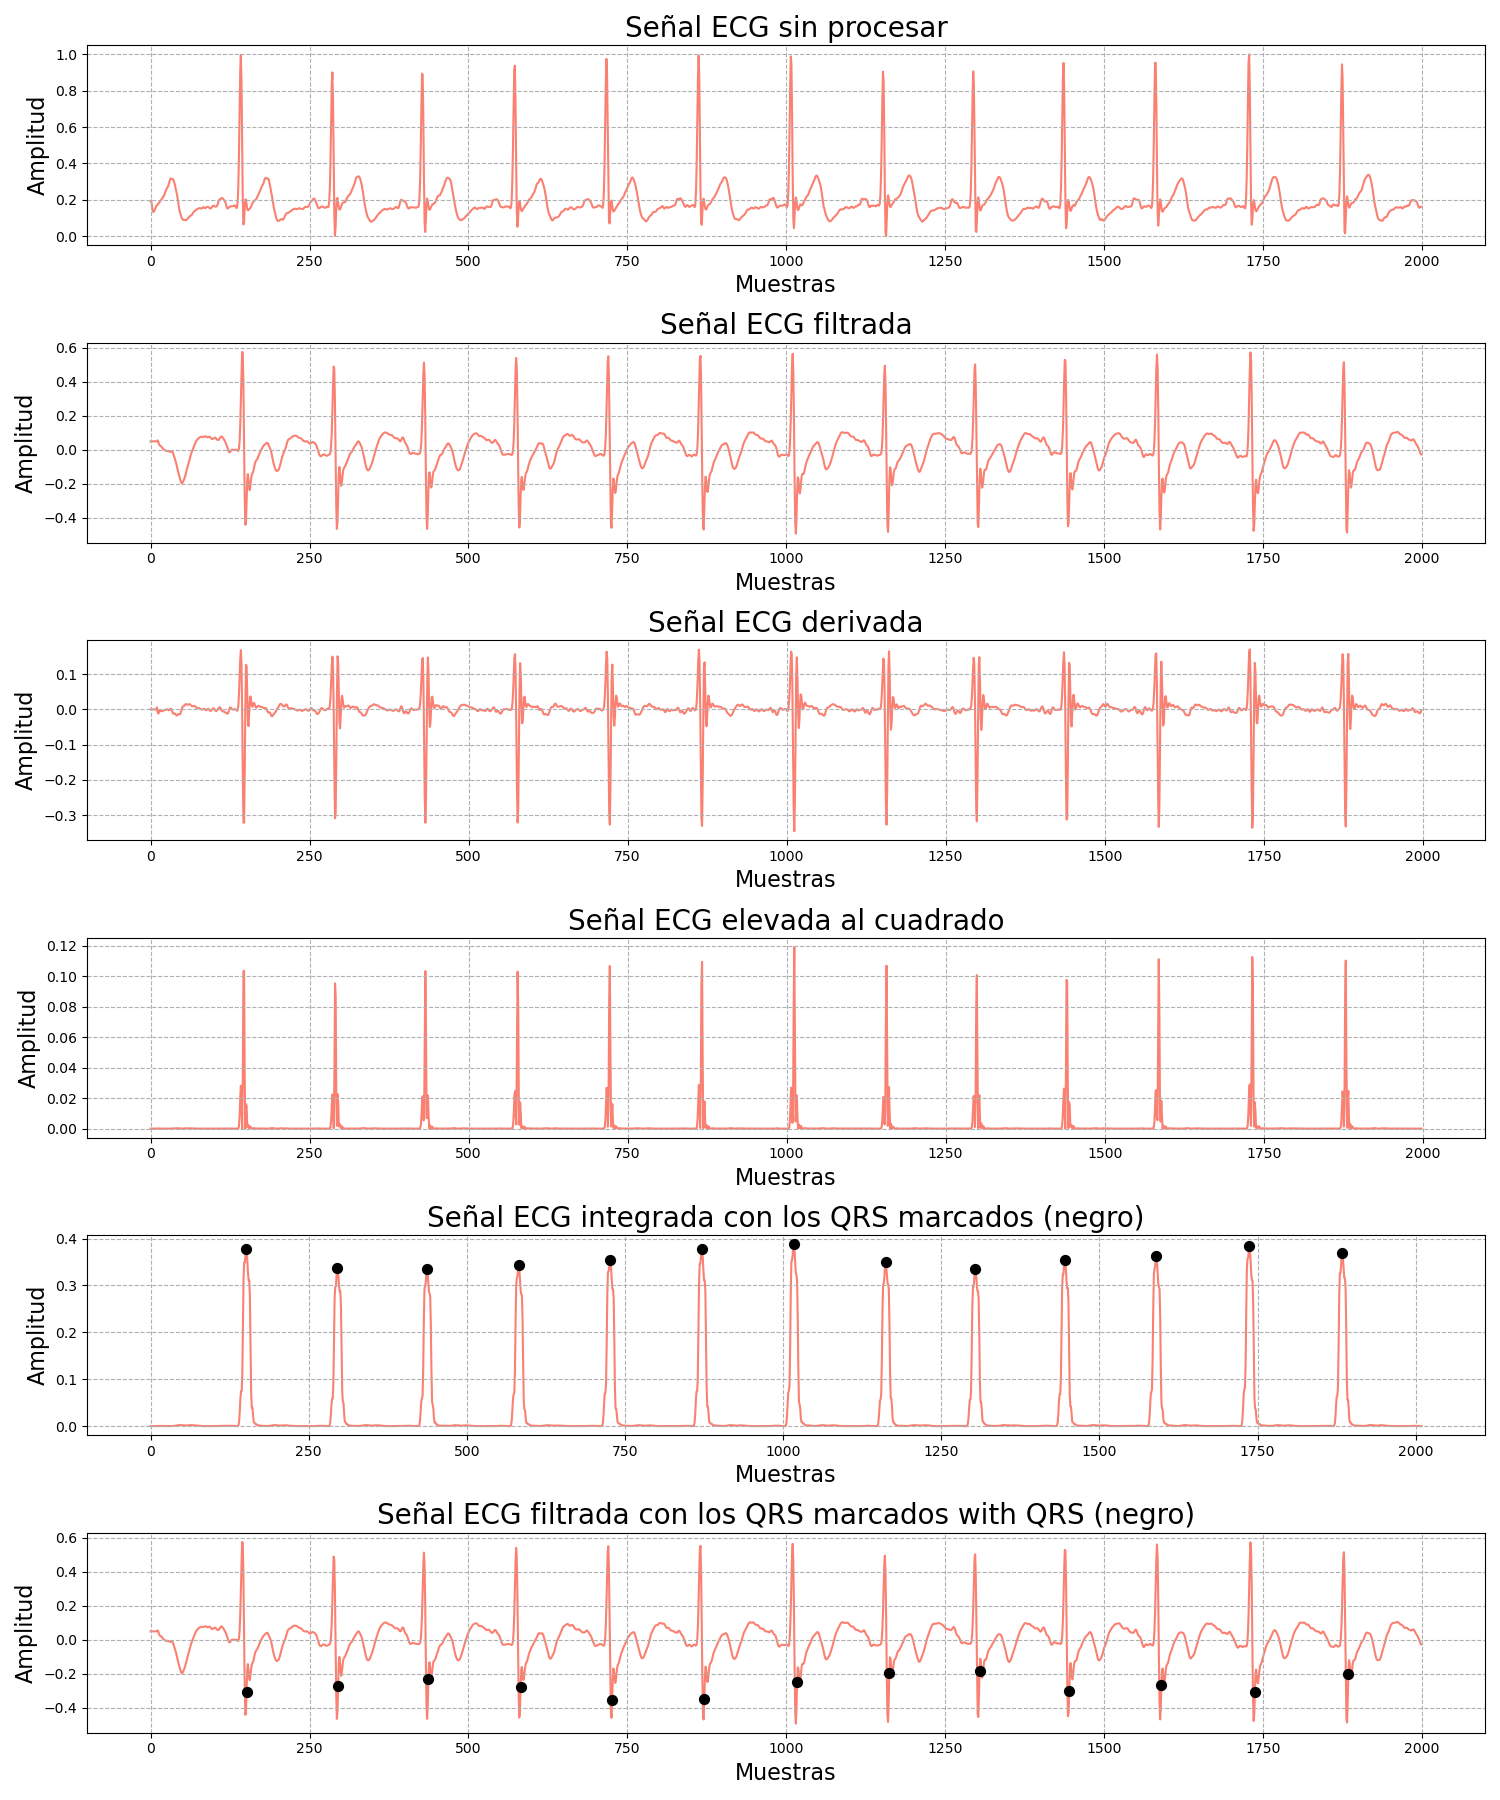
\includegraphics[width=0.5\textwidth]{/pan_2}
	\caption{Detecci�n de QRS con el algoritmo de Pan-Tompkins.}
	\label{pan}
\end{figure}

En un inicio, se utiliz� una implementaci�n  del algoritmo de Pan-Tompkins para la detecci�n de los complejos QRS \cite{pan}. Este algoritmo se basa en la derivaci�n, la elevaci�n al cuadrado y la integraci�n de la se�al, para la detecci�n de picos basada en umbrales adaptativos, como se puede ver en la Figura \ref{pan}.

Sin embargo, para detectar los picos R con mayor precisi�n, se ha utilizado una herramienta de detecci�n de picos de \textit{SciPy.org} \cite{picos}, definiendo un umbral sobre las se�ales normalizadas y fijando una distancia m�nima entre picos, que se corresponde con el intervalo R-R, y que var�a en funci�n de si la persona ha hecho ejercicio o no. Este valor se ha establecido de manera fija pero, habiendo obtenido previamente el n�mero de complejos QRS mediante el algoritmo de Pan-Tompkins, se podr�a hacer din�mico en funci�n del n�mero de latidos, mejorando as� la detecci�n. 

%Podria haber usado el pan-tomkins para calcular el n�mero de latidos, y as� hacer una distancia din�mica en funci�n del n�mero de latidos segun ha hecho deporte o no xq ritmo card�aco var�a
\begin{figure}[h!]
	\centering
	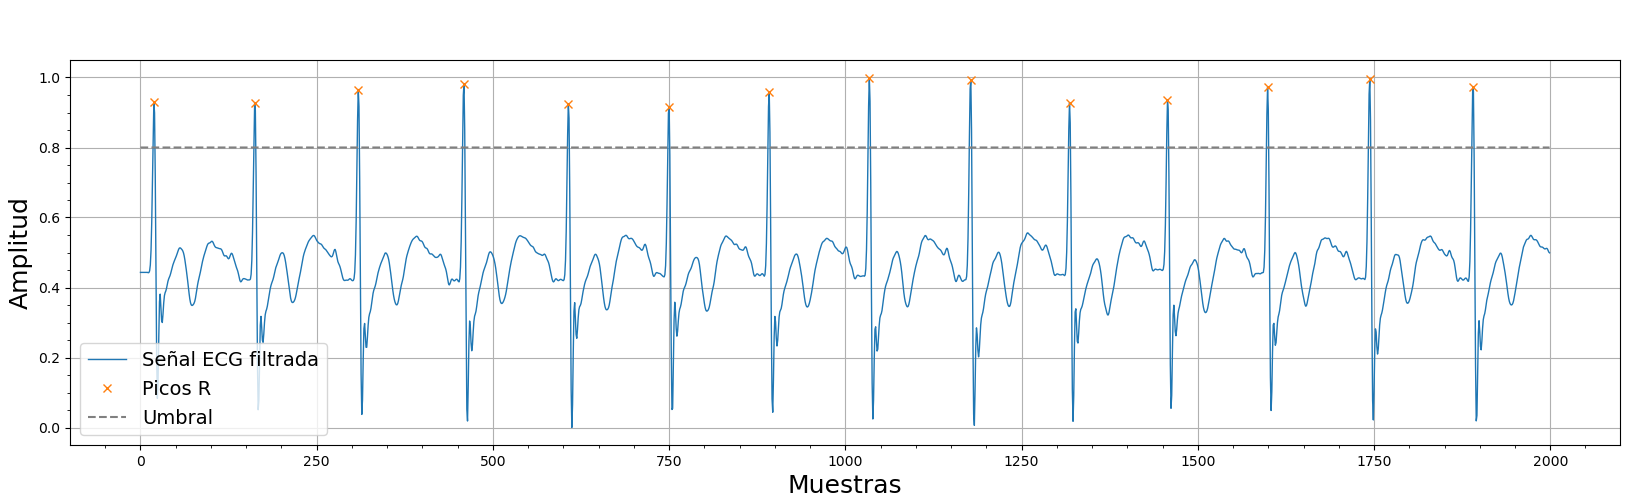
\includegraphics[width=1\textwidth]{/picos}
	\caption{Detecci�n de picos R.}
	\label{picos}
\end{figure}	

Esta tarea ha sido especialmente complicada, pues en muchas de las se�ales la presencia de ruido a�n despu�s del filtrado o la propia morfolog�a de la se�al de ciertas personas, hace que el pico R no siempre sea f�cil de distinguir, confundi�ndose en muchas ocasiones con la onda T. Una posible mejora es la aplicaci�n de un umbral din�mico basado en la media m�vil de la se�al. Por otro lado, como medida preventiva, aquellas se�ales en las que no se ha detectado un m�nimo de 3 picos R han sido descartadas, considerando que la detecci�n no se ha realizado correctamente. 

%FIGURA de umbral din�mico???

Una vez localizados los picos R, se ha llevado a cabo la segmentaci�n de la se�al en los diferentes complejos QRS. Para ello: 
\begin{itemize}
	\item Se aplica una ventana de 0,125 segundos a cada punto detectado, obteniendo as� un vector H de \textit{n} complejos QRS, y el resto de la se�al se desecha. Este valor es constante, pues como se ha podido ver en la Figura \ref{qrss} %la del QRS superpuesto con y sin deporte
	  la duraci�n del QRS no var�a para una misma persona a�n habiendo realizado ejercicio, aunque el ritmo card�aco sea mayor. 
	\item De estos \textit{n} QRS, se extraen los \textit{m} QRS m�s discriminatorios, obteniendo as� el \textbf{vector V}, que es el vector que va a caracterizar a cada sujeto junto con su correspondiente etiqueta: 
	\begin{itemize}
		\item Para valorar la calidad de los complejos QRS y obtener dichos \textit{m} QRS m�s discriminatorios que forman el vector \textbf{V}, se extrae del vector H el QRS promedio, $\overline{QRS}$, y se calculan los coeficientes de correlaci�n de Pearson. Es decir, se calcula la correlaci�n entre cada complejo QRS del vector H y el $\overline{QRS}$, obteniendo el vector C.
		\item Los \textit{m} complejos QRS que tengan mayor valor de C se concatenan, dando como resultado el vector \textbf{V}.
		\item Si el n�mero \textit{i} de QRS presentes en el vector H es menor que \textit{m}, se completa el vector \textbf{V} replicando el complejo que tenga mayor valor de C.  
		\item Si el valor del coeficiente de correlaci�n de Pearson es menor de 0,5, se considera que el complejo QRS no est� correlado con el $\overline{QRS}$, y por tanto se descarta considerando que es ruidoso, o un complejo mal detectado. 
		
	\end{itemize}
\end{itemize}

\begin{figure}[H]
	\centering
	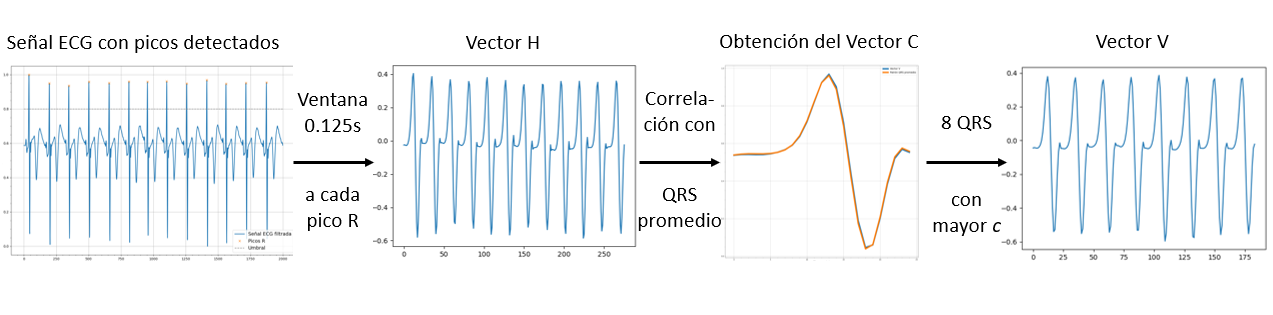
\includegraphics[width=1\textwidth]{/preproceso_3}
	\caption{Proceso de la segmentaci�n de la se�al hasta la obtenci�n del vector V.}
	\label{preproceso}
\end{figure}



Para cada muestra que, recordamos, tiene una duraci�n de 10 segundos y un n�mero de QRS variable, sobre todo, seg�n la persona y en funci�n de si ha realizado ejercicio o no, se extrae el vector \textbf{ V} de caracter�sticas fijando $\textit{m} = 8 QRS$, es decir, un vector de 1 sg compuesto por 8 QRS concatenados y una dimensi�n de $200 \times 1$, teniendo en cuenta la frecuencia de muestreo (200 Hz). Este valor para \textit{m} se ha fijado teniendo en cuenta el art�culo de referencia \cite{deepecg}, que basa su decisi�n en estudios previos que demuestran que 8 latidos mantienen un buen equilibrio entre rendimiento y usabilidad \cite{Odinaka2012}. Adem�s, el estudio de Salloum \textit{et al.} \cite{autentiguia}, tambi�n ha demostrado que un mayor n�mero de latidos concatenados da lugar a un mejor rendimiento de la red neuronal. % (9 latidos concatenados frente a 3 en este estudio).

\begin{figure}[H]
	\centering
	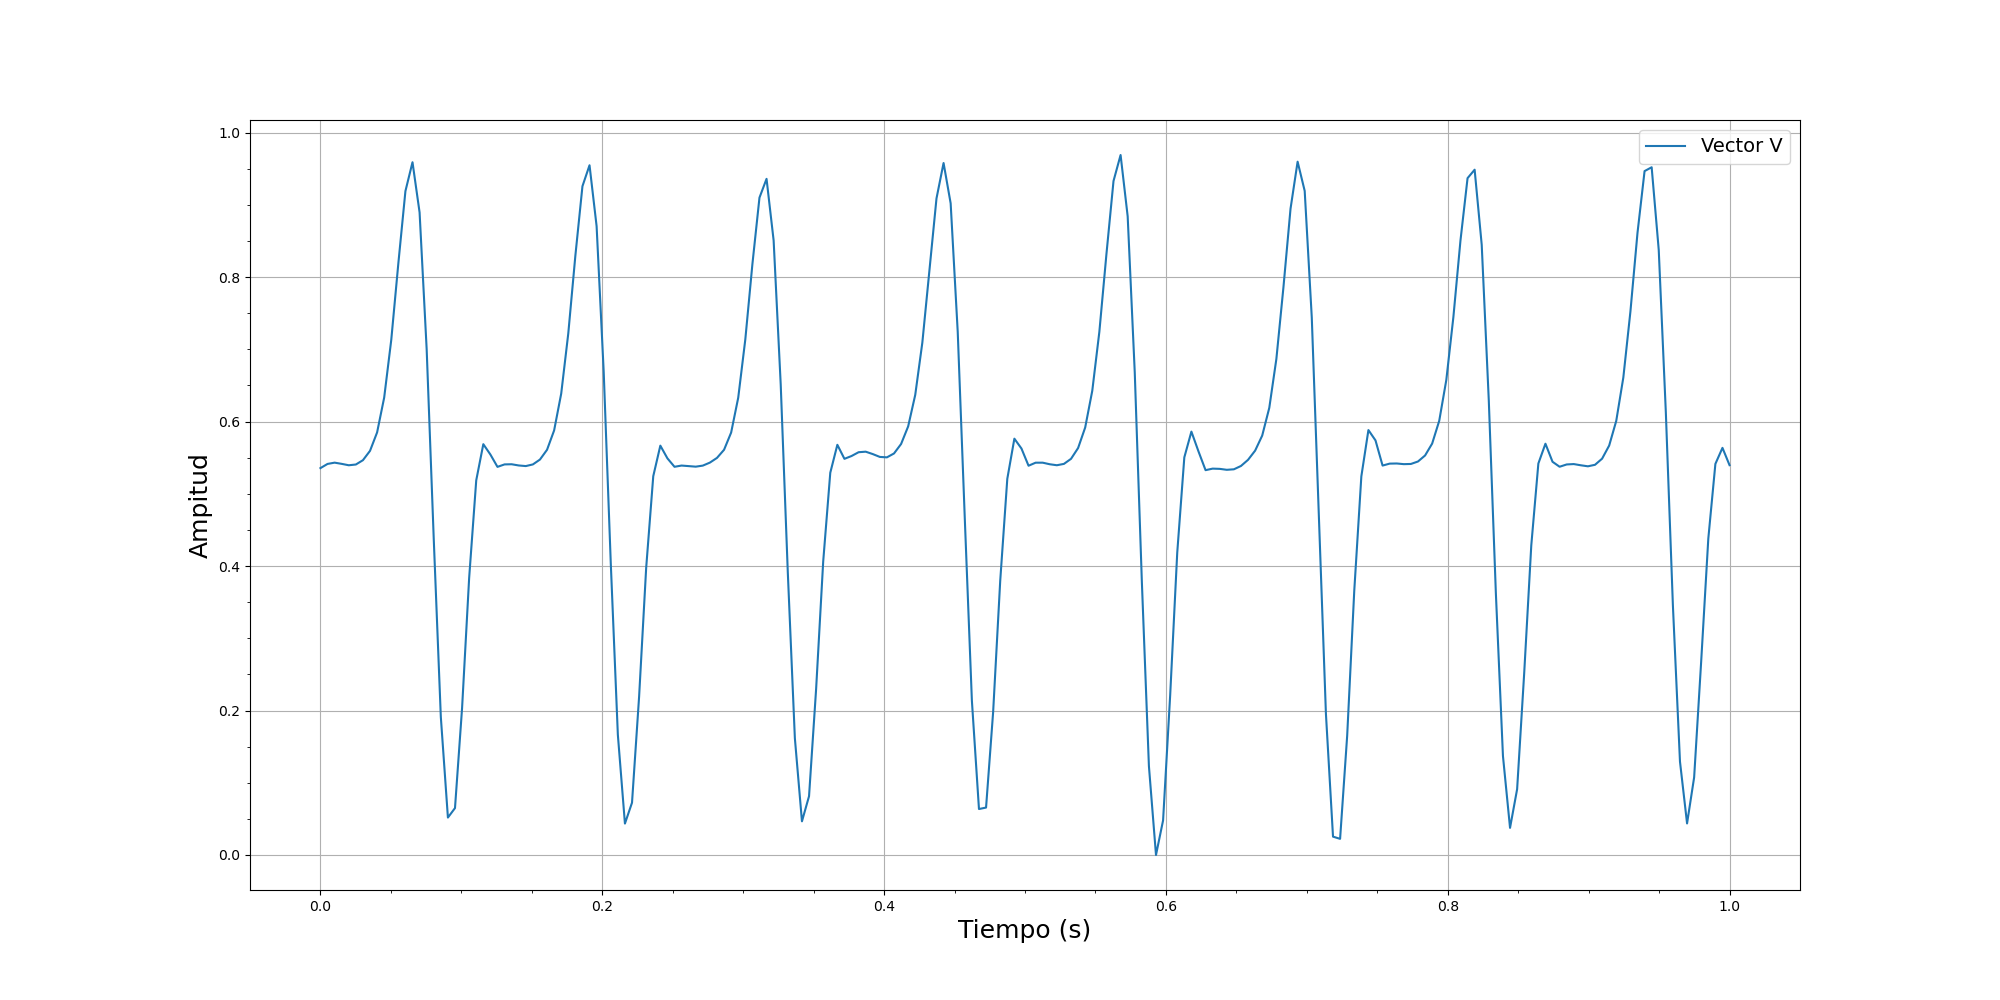
\includegraphics[width=0.7\textwidth]{/vectv}
	\caption{Ejemplo de un vector V, compuesto por 8 QRS y tiene 1 segundo de duraci�n. El vector V es la entrada de la CNN.}
	\label{v}
\end{figure}

A partir de este momento, cada vez que se haga referencia al uso de muestras de un usuario, �stas equivalen al \textbf{V}. Este vector est� compuesto por 200 elementos \break(1 segundo).
 
\section{Extracci�n de caracter�sticas}

%z-score normalization si me faltan cosas aqu�

Una vez realizado el preprocesamiento de la se�al y obtenido el vector V, que se va a emplear para caracterizar a los sujetos, el siguiente paso es la extracci�n de caracter�sticas, es decir, la b�squeda de patrones. Como ya se ha comentado anteriormente, para realizar tanto la funci�n de identificaci�n como de autenticaci�n, la extracci�n de caracter�sticas se basa en una red neuronal convolucional (CNN). 

Aunque el uso m�s generalizado de las CNNs es la clasificaci�n de im�genes 2D, su aplicaci�n para se�ales unidimensionales es tambi�n muy efectiva cuando se espera extraer rasgos de peque�as ventanas del conjunto de datos, y cuando la ubicaci�n de estas caracter�sticas dentro de la ventana no es de gran relevancia %\cite{la pag web que he utilizado}.
As�, mientras que una capa densamente conectada (\textit{fully connected}) aprende patrones globales en su espacio global de entrada, las capas convolucionales lo hacen de manera local \cite{Torres2018}. 

%Escribir algo m�s sobre redes neuronales�?

Como se va a detallar a lo largo de esta secci�n, para la identificaci�n de usuarios y el entrenamiento de la red, el reconocimiento de los patrones obtenidos por la CNN se lleva a cabo mediante una capa de salida con la funci�n de activaci�n \textit{Soft-max}, que devuelve la identidad del sujeto, mientras que para la autenticaci�n, se realiza una comparaci�n de estos patrones obtenidos por la CNN, determinando la verificaci�n de la identidad en funci�n de un umbral. 

Los pasos que se han seguido para ello son: el dise�o de la arquitectura de la CNN, la selecci�n de hiperpar�metros y el entrenamiento de la red y, en autenticaci�n, la comparaci�n de patrones.

%\nameref{arq}, la \nameref{hiper} y, en autenticaci�n, la \nameref{matchin}. Todos ellos se han aplicado tanto para la primera base de datos como para la segunda. 
%Algo m�s�?

\subsection{Arquitectura de la CNN} \label{arq}

La Figura \ref{fig:arq} muestra la arquitectura de la red utilizada. Como se puede comprobar, las primeras capas son convolucionales, intercaladas con capas de reagrupamiento \textit{pooling} y de normalizaci�n, seguidas por una capa de  \textit{dropout} y finalmente, para el entrenamiento y la identificaci�n, una capa densamente conectada (\textit{fully connected}) con activaci�n \textit{Soft-max} (que se elimina en la configuraci�n de red para autenticaci�n de usuarios).

\begin{figure}[H]
	\centering
	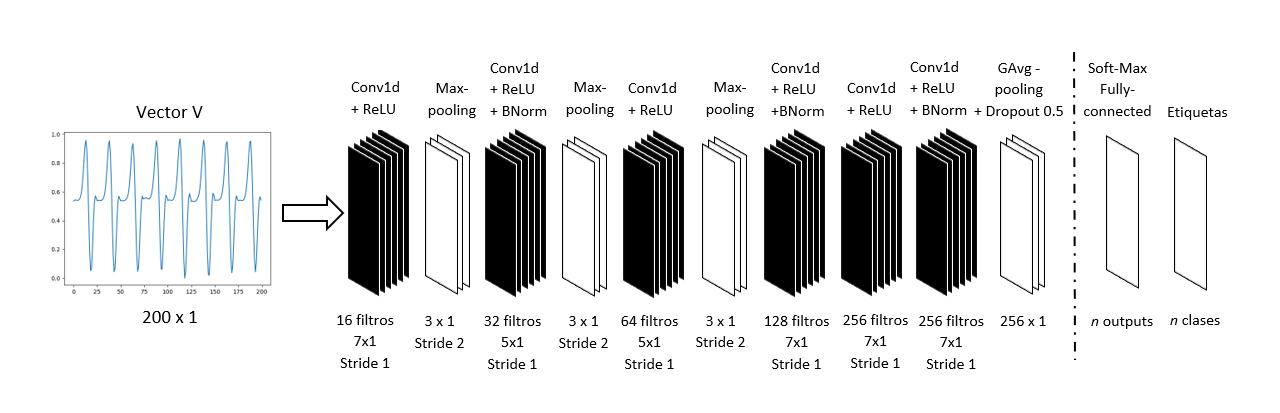
\includegraphics[width=1\textwidth]{/arquitectura}
	\caption{Esquema de la arquitectura de la CNN. La capa densamente conectada solo se utiliza para el entrenamiento de la red y para identificaci�n.}
	\label{fig:arq}
\end{figure}

%un peqe�o resumen de lo que hace cada capa �?
A continuaci�n, vamos a analizar brevemente las diferentes capas y su comportamiento:
\begin{itemize} 
	\item Primera capa convolucional 1D: esta capa es la que recibe los datos de entrada, es decir, el vector V obtenido tras el preprocesado de las se�ales. Este vector tiene una dimensi�n de $200 \times 1$, y por tanto, la capa estar� compuesta por 200 neuronas. Esta capa define 16 filtros de dimensi�n $7 \times 1$, conocida como \textit{kernel size}, es decir, la red aplica 16 filtros diferentes sobre el vector de entrada. Como resultado de la convoluci�n con cada filtro, la salida de esta capa va a ser una matriz de caracter�sticas de $194 \times 16$. Cada columna de esta matriz contiene los pesos (\textit{weights}) de un �nico filtro, es decir, 194 pesos. Estos pesos se van optimizando conforme se va entrenando la red. 
	
	\item\textit{Max-pooling}: esta capa se utiliza despu�s de una capa convolucional con el fin de simplificar la informaci�n recogida por �sta y crear una versi�n condensada de la informaci�n que contiene. De esta manera, se reduce la complejidad de la salida de la capa anterior y ayuda a prevenir el sobreajuste \textit{overfitting} de los datos. En concreto, la capa \textit{Max-pooling} se queda con el valor m�ximo de los que hab�a en la ventana de entrada. En este caso, tiene un tama�o de 3, por lo cual el tama�o de la matriz de salida de esta capa ser� solo una tercera parte de la de entrada. 
	
	\item\textit{Batch Normalization}: esta capa normaliza las funciones de activaci�n de la capa anterior para cada \textit{batch}, es decir, aplica una transformaci�n para mantener su media pr�xima a 0 y su desviaci�n est�ndar pr�xima a 1. Esta capa ayuda a prevenir la realentizaci�n del entrenamiento, reduciendo el cambio de covariable interno (del ingl�s \textit{internal covariate shift}). El tama�o de la salida de esta capa es el mismo que el de la entrada. 
	
	\item\textit{Global Average Pooling}: esta capa es otro tipo de reagrupamiento, donde cada grupo de puntos de entrada se transforma en el valor promedio de los mismos, en vez del valor m�ximo. Por tanto, por cada filtro, solo permanece en la red un peso, reduci�ndose as� a una sola dimensi�n la salida. 
	
	\item\textit{Dropout}: esta capa asignar� aleatoriamente un 0 a los pesos de las neuronas de la red. En este caso, el $50\%$ de las neuronas recibir�n un peso igual a cero. Gracias a esta capa, la red es menos sensible a peque�as variaciones en los datos, y por tanto, aumentar� su rendimiento cuando se utilice para datos desconocidos, es decir, mejorar� su capacidad de generalizar. La dimensi�n de la salida de esta capa es la misma que la de entrada. 
\end{itemize}

Para todas las capas convolucionales se usa la funci�n de activaci�n ReLU (\textit{Rectified Linear Units}) para introducir la no linealidad a la red. La funci�n de activaci�n ReLU activa un solo nodo si la entrada est� por encima de cierto umbral. Si la entrada est� por debajo de cero la salida ser� cero, y cuando est� por encima, la salida es una relaci�n lineal con la variable de entrada de la forma $f(x) = x$. Adem�s, en todas las capas \textit{Max-pooling} se especifica una longitud de paso de avance (\textit{stride}) de 2. Este par�metro controla c�mo convoluciona el filtro sobre el volumen de entrada, es decir, define el n�mero de pasos en que se mueve la ventana de los filtros, reduciendo todav�a m�s el tama�o de la matriz de salida de las capas. 

\newpage
Las capas convolucionales y de reagrupamiento se van intercalando, como ya se ha visto en la Figura \ref{fig:arq}, de forma que la informaci�n obtenida como resultado de la convoluci�n de los diferentes filtros con la se�al de entrada se condensa, hasta que se obtiene un �nico \textbf{vector de caracter�sticas} de 256 elementos. Este vector representa el patr�n de cada usuario. La Figura \ref{fig:summary} muestra la arquitectura de la red con los tama�os de salida de cada capa. 

\begin{figure}[H]
	\centering
	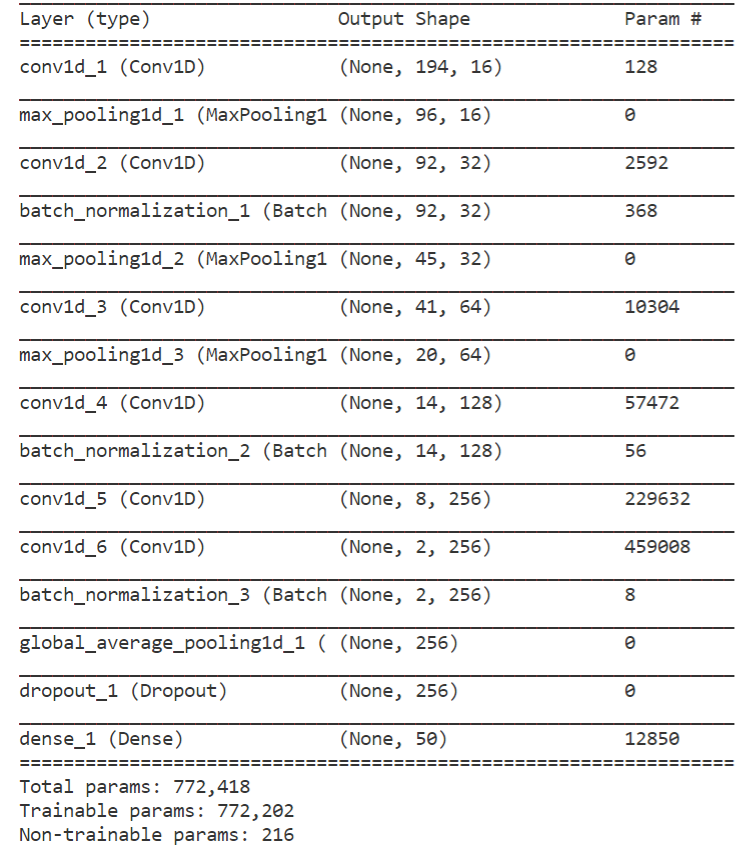
\includegraphics[width=0.6\textwidth]{/model}
	\caption{Resumen del modelo empleado con los tama�os de las salidas de cada capa.}
	\label{fig:summary}
\end{figure}

Los par�metros que no son entrenables provienen de las capas de  \textit{Batch Normalization}, pues sus vectores de media y varianza no se actualizan por propagaci�n hacia atr�s (\textit{backpropagation}) \cite{github}. 

En el caso de la arquitectura de la red para el entrenamiento y para realizar identificaci�n, se utiliza una �ltima capa de salida densamente conectada con funci�n de activaci�n \textit{Soft-max}. Esta capa recibe como entrada el vector de caracter�sticas o patr�n, de 256 elementos, y lo clasifica, de forma que devuelve como salida un vector de dimensi�n igual al n�mero de clases posibles en la clasificaci�n. Por tanto, para la primera base de datos que tiene 50 usuarios registrados, el vector tendr� 50 elementos, y para la segunda que tiene 55, 55. En esta capa \textit{Soft-max}, cada neurona depende de las salidas de todas las dem�s neuronas de la capa, puesto que la suma de la salida de todas ellas debe ser 1. Por tanto, el valor de salida de cada neurona representa la probabilidad que tiene de pertenecer a la clase que representa. 

%N neurons (where N is the number of subjects),

Por otro lado, en autenticaci�n, el vector de caracter�sticas se utiliza para realizar \textit{template matching}, como se explica en la secci�n \ref{matchin}.
%Pero como hemos explicado, no se conectan todas las neuronas de entrada con todas las neuronas de este primer nivel de neuronas ocultas, como en el caso de las redes neuronales densamente conectas; solo se hace por peque�as zonas localizadas del espacio de las neuronas de entrada que almacenan los p�xeles de la imagen.
\subsection{Selecci�n de hiperpar�metros y entrenamiento de la red} \label{hiper}

Los hiperpar�metros difieren de los par�metros del modelo de una red, en que estos no pueden ser aprendidos expl�citamente de los datos durante la fase de entrenamiento. Por tanto, los hiperpar�metros se definen antes de entrenar un modelo y rigen el propio proceso de entrenamiento, influyendo de manera muy significativa en el resultado final. El n�mero de hiperpar�metros que se puede tener en cuenta a la hora de dise�ar una red es muy extenso, y existen muchas posibles combinaciones. Adem�s, tambi�n hay muchas formas de llevar a cabo la optimizaci�n de dichos hiperpar�metros. Esto hace que su proceso de selecci�n y optimizaci�n sea muy laborioso. 

Para llevar a cabo esta optimizaci�n, los datos de entrenamiento han sido a su vez divididos en dos subconjuntos (\textit{datasets}): el de entrenamiento y el de validaci�n. De esta forma, los datos de validaci�n, que la red no ha analizado durante el entrenamiento, se utilizan para ajustar los hiperpar�metros. As�, para ambas bases de datos, las muestras se han dividido desde el principio en tres \textit{datasets}: entrenamiento, validaci�n y prueba. De esta manera, el modelo siempre se entrena sobre los datos de entrenamiento, los hiperpar�metros se optimizan usando los datos de validaci�n y el resultado final del modelo se eval�a sobre los de prueba, conocido como m�todo de retenci�n (\textit{holdout method}). La desventaja que presenta este m�todo es que la evaluaci�n de resultados se ve condicionada por los datos elegidos para la validaci�n. Por ello, para la primera base de datos, tambi�n se ha probado una validaci�n cruzada de K iteraciones (\textit{k-fold cross-validation}). En ella, los datos de entrenamiento se dividen en $k$ subconjuntos (\textit{folds}), y el proceso de validaci�n cruzada se repite $k$ veces. En cada iteraci�n, uno de los $k$ subconjuntos se usa como set de validaci�n y el  resto $k-1$ subconjuntos son utilizados como set de entrenamiento. Finalmente se realiza la media aritm�tica de los resultados de cada iteraci�n para obtener un �nico resultado. Sin embargo, aunque este m�todo es m�s preciso, es muy lento desde el punto de vista computacional, y no se ha aplicado para la segunda base de datos. 

El m�todo de muestreo que se ha utilizado durante la optimizaci�n ha sido el muestreo de cuadr�cula (\textit{grid search}), que consiste en una b�squeda exhaustiva sobre determinados conjuntos de hiperpar�metros del modelo. La red es entrenada para cada valor de los hiperpar�metros, y el resultado de cada modelo es comparado, eligiendo finalmente el que que haya obtenido un resultado mejor. La m�trica que se ha utilizado para comparar los modelos es el rendimiento (\textit{accuracy}). 


\begin{table}[H]
	\centering
	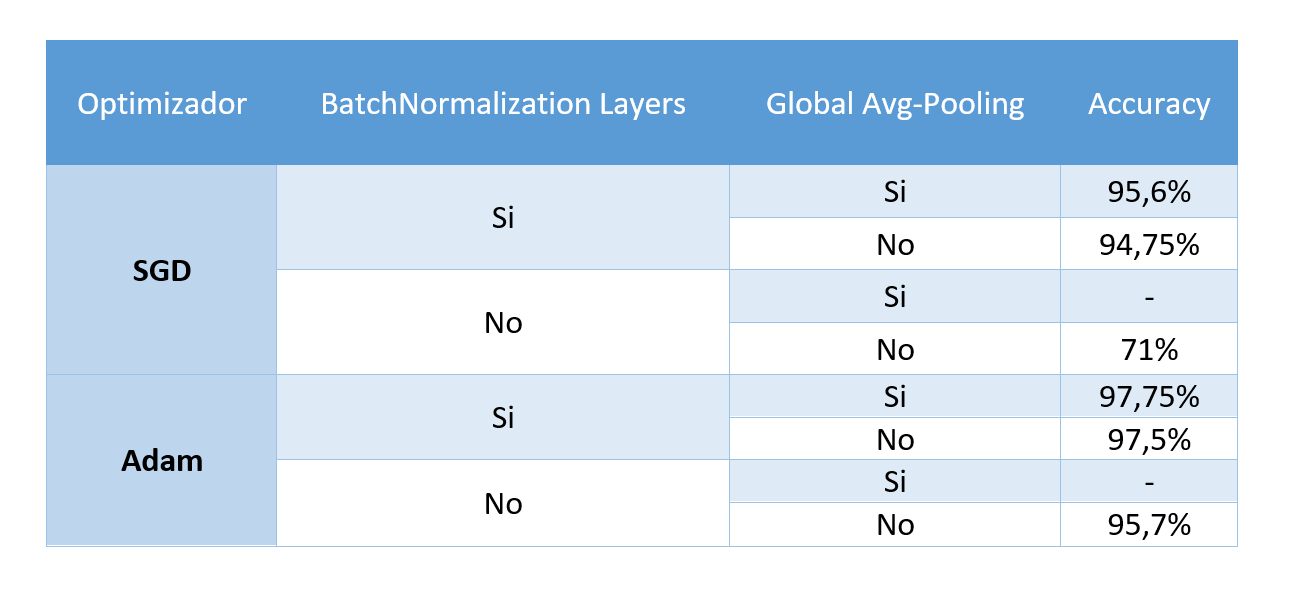
\includegraphics[width=0.75\textwidth]{/compa}
	\caption{Comparativa de los resultados del rendimiento de la red durante la fase de prueba para diferentes modelos.}
	\label{compa}
\end{table}

Algunos de los hiperpar�metros, como el n�mero de capas ocultas de la red, el uso de \textit{strides}, el tama�o y n�mero de filtros y las funciones de activaci�n, entre otros, ya se han comentado en la secci�n anterior. Estos han sido ajustados bas�ndose en el art�culo de referencia \cite{deepecg} y de manera emp�rica. La Tabla \ref{compa} muestra una comparativa de los resultados de rendimiento sobre los datos de prueba de diferentes modelos que se han evaluado para la primera base de datos. 


Otros hiperpar�metros que se han tenido en cuenta son el tama�o de \textit{batch} y el n�mero de \textit{epochs}. Para ambas bases de datos, se ha realizado un muestreo en cuadr�cula para diferentes valores. Los resultados de rendimiento obtenidos para cada base de datos sobre las muestras de prueba en las diferentes combinaciones se pueden ver en la Figura \ref{batch}.

\begin{figure}[H]
	\centering
	\subfigure[Base de datos 1]{
		\label{fig:bd1}
		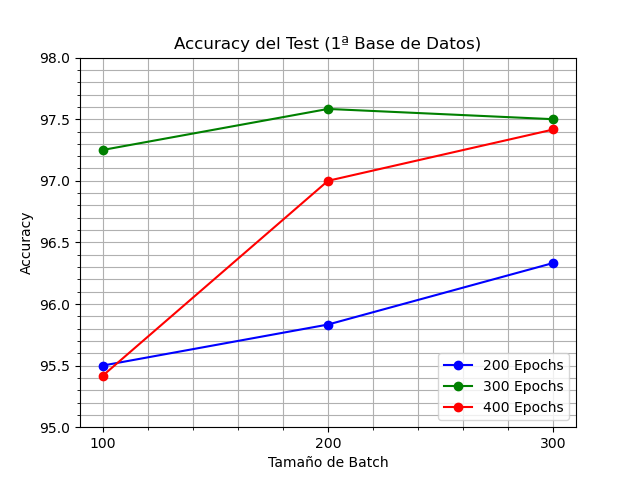
\includegraphics[width=0.6\textwidth]{/acc_epo_1}}
	\subfigure[Base de datos 2]{
		\label{fig:bd2}
		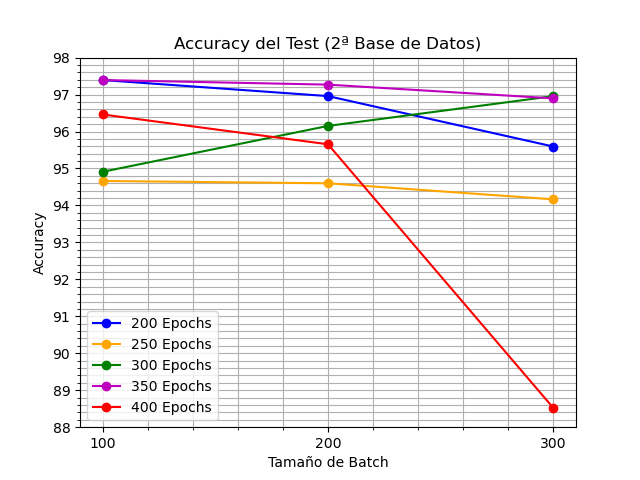
\includegraphics[width=0.6\textwidth]{/acc_epo_2}}

	\caption{Optimizaci�n del tama�o de \textit{batch} y el n�mero de \textit{epochs} mediante un muestreo de cuadr�cula.}
	\label{batch}
\end{figure}


Para la fase de entrenamiento la funci�n de p�rdida (\textit{loss}) que se ha utilizado es \break \textit{categorical\_crossentropy}, que ajusta los par�metros del modelo (los pesos $wi$ y el sesgo $b$) de tal manera que el resultado de la p�rdida tenga el m�nimo valor posible.
Finalmente, el optimizador usado ha sido el \textit{adam} con una tasa de aprendizaje (\textit{learning rate}) de  0.001.


La Figura \ref{fig:accloss} muestra la evoluci�n del rendimiento y de la p�rdida durante el entrenamiento de uno de los modelos. Como se puede ver, tanto para el set de entrenamiento como para el de validaci�n, el rendimiento se acerca a 1 y la p�rdida a 0, obteni�ndose por tanto buenos resultados en cuanto al entrenamiento de la red. 

\begin{figure}[H]
	\centering
	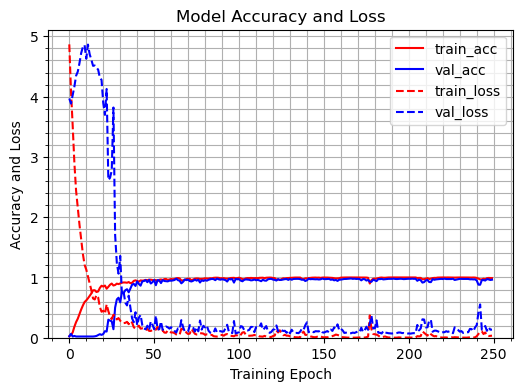
\includegraphics[width=0.7\textwidth]{/acc_loss_}
	\caption{Evoluci�n del rendimiento y de la p�rdida de entrenamiento y de validaci�n durante la fase de entrenamiento de la red.}
	\label{fig:accloss}
\end{figure}


\subsection{Comparaci�n de patrones} \label{matchin}

%Una vez obtenida la representaci�n de la muestra en el nuevo espacio K-dimensional, se
%utilizan los coeficientes para comparar entre muestras. Para realizar esta comparaci�n se
%va a utilizar la Distancia Eucl�dea normalizada:
%??(??1, ??2) =
%1
%??
%?(??1 ? ??2)?? (??1 ? ??2)
%Trabajo de Investigaci�n
%Concurso de Acceso a Catedr�tico de Universidad en UC3M (DF000755/56)
%Dr. Ra�l S�nchez Re�llo 37
%Con la distancia obtenida, dependiendo de si el sistema se configura en modo
%Identificaci�n o en Autenticaci�n, se utilizar� o la votaci�n de vecino m�s pr�ximo (en
%Identificaci�n), o la comparaci�n con un umbral previamente establecido (en
%Autenticaci�n).
%Lo especialmente atractivo de esta aproximaci�n es su bajo coste computacional, que
%permitir� su ejecuci�n en tiempo real y sin unas demandas de procesamiento excesivas


%For the authentication scenario, the equal error
%rate (EER) was computed in the following manner. Given a
%summary vector obtained from the evaluation data of a particular
%subject, this vector is compared to each enrollment model
%(one model for each subject in the enrollment/evaluation set)
%using cosine distance as a similarity metric. An authentication
%decision for each comparison is then made based on a given
%threshold. Thus, for each summary vector obtained from the
%evaluation dataset, there is a certain number of each of the following
%quantities: true acceptance, true rejection, false acceptance,
%false rejection. Each of these 4 quantities is summed
%across the set of summary vectors obtained from the evaluation
%dataset, and the false acceptance rate (FAR) and false
%rejection rate (FRR) are computed. The threshold is then varied
%to yield a plot of FAR and a plot of FRR, and the EER is
%taken to be the intersection of these two curves.

%La comparaci�n de patrones, o \textit{template matching} 
La autenticaci�n biom�trica se ha llevado a cabo mediante la comparaci�n de patrones o \textit{template matching}. M�s espec�ficamente, un \textbf{patr�n o \textit{template}} es una instancia registrada de las caracter�sticas biom�tricas de una persona. El patr�n se registra durante la fase de reclutamiento del usuario en el sistema y se almacena en una base de datos. Posteriormente, cuando el usuario realiza una consulta (\textit{query}), se registra una nueva muestra  y se compara con su patr�n espec�fico, en oposici�n a la identificaci�n, en la que se compara con todos los patrones registrados, tal y como se ha explicado en la secci�n \ref{idvsau}.

Para implementar la configuraci�n de red utilizada en autenticaci�n, se ha retirado la �ltima capa (\textit{Soft-max}) de un modelo entrenado con los usuarios de la primera base de datos, y esta nueva arquitectura de red se ha utilizado para verificar la identidad de los usuarios de la segunda base de datos, y viceversa. De esta manera, la red siempre ha sido entrenada con usuarios diferentes a los usuarios que se quiere autenticar. 

Durante la fase de reclutamiento, la red se utiliza para obtener el patr�n espec�fico de cada usuario. La nueva salida (\textit{output}) de la red es el vector de car�cter�sticas de 256 elementos para cada muestra, como ya coment�bamos en \ref{arq}. De todos los vectores de caracter�sticas obtenidos para un mismo usuario, se extrae un �nico vector promedio, de la misma dimensi�n, y �ste se almacena como \textbf{patr�n} del usuario. 
 
%PONER AQUI LAS TSNE Y PCAS O EN RESULTADOS. 

Durante la fase de consulta, se obtiene el vector de caracter�sticas para una nueva muestra del usuario que realiza dicha consulta, y este vector de caracter�sticas se compara con el patr�n almacenado de este usuario. Para realizar esta comparaci�n, en el espacio de dimensi�n $k = 256$, se ha utilizado la distancia eucl�dea: 
\begin{center}
	$D(P,Q) = \sqrt{\sum\limits_{i=1}^{n}(p_i - q_i)^{2}}$
\end{center}

Donde $P$ es el vector \textbf{patr�n} y $Q$ es el vector de la  \textbf{consulta (\textit{query})}. Si la distancia obtenida es menor que un umbral establecido, la consulta se considera v�lida, el usuario es quien dice ser, mientras que si supera el umbral la consulta es rechazada, pues el usuario no es quien dice ser sino un impostor. 

%!TEX root = ../../Principal/TFG.tex
\chapter{Evaluaci�n del sistema: resultados experimentales}
\label{chap:resultados}
\pagestyle{fancy}
\thispagestyle{empty}
%
\graphicspath{{../Desarrollo/Imagenes/}}
\DeclareGraphicsExtensions{.pdf,.jpg,.png}
%\
En este cap�tulo se va a describir la evaluaci�n de la red neuronal convolucional propuesta en el cap�tulo anterior con las bases de datos, tambi�n ya descritas. Los resultados est�n divididos en dos secciones: \nameref{id} y \nameref{aut}. Adem�s, los resultados de identificaci�n est�n a su vez divididos seg�n las diferentes bases de datos. 


\section{Identificaci�n} \label{id}

La arquitectura de identificaci�n se ha probado tanto para la primera base de datos como para la segunda y, adem�s, se ha realizado una prueba sobre la base de datos completa (los 105 sujetos). En todos los casos, se ha realizado una identificaci�n sobre un conjunto cerrado (\textit{closed set}), es decir, todos los sujetos que se pretende identificar han tenido que ser previamente registrados (todas las muestras de test pertenecen a usuarios cuyas muestras se han utilizado para el entrenamiento de la red).

Las muestras se han dividido siempre en un 80\% para entrenamiento y 20\% para test. A su vez, el set de entrenamiento se ha dividido en un 90\% entrenamiento y 10\% validaci�n. 

Al evaluar el rendimiento del clasificador con ambas bases de datos, se ha querido comprobar que, efectivamente, ni el estado f�sico de la persona ni el d�a en que han sido tomadas las muestras afectan al proceso de su identificaci�n. 


\subsection{Primera base de datos}


Para los primeros 50 usuarios, se han utilizado muestras tanto de la primera sesi�n como de la segunda de cada uno. Adem�s, se han incluido muestras tanto con los ojos abiertos como con los ojos cerrados. Como resultado, se ha conseguido un rendimiento de prueba del $97.58\%$, con una p�rdida de $0.08$.



Para llevar a cabo una evaluaci�n m�s exhaustiva del clasificador, la matriz de confusi�n con las identidades reales y las predichas se puede ver en la Figura  \ref{fig:cm1}. 

\begin{figure}[H]
	\centering
	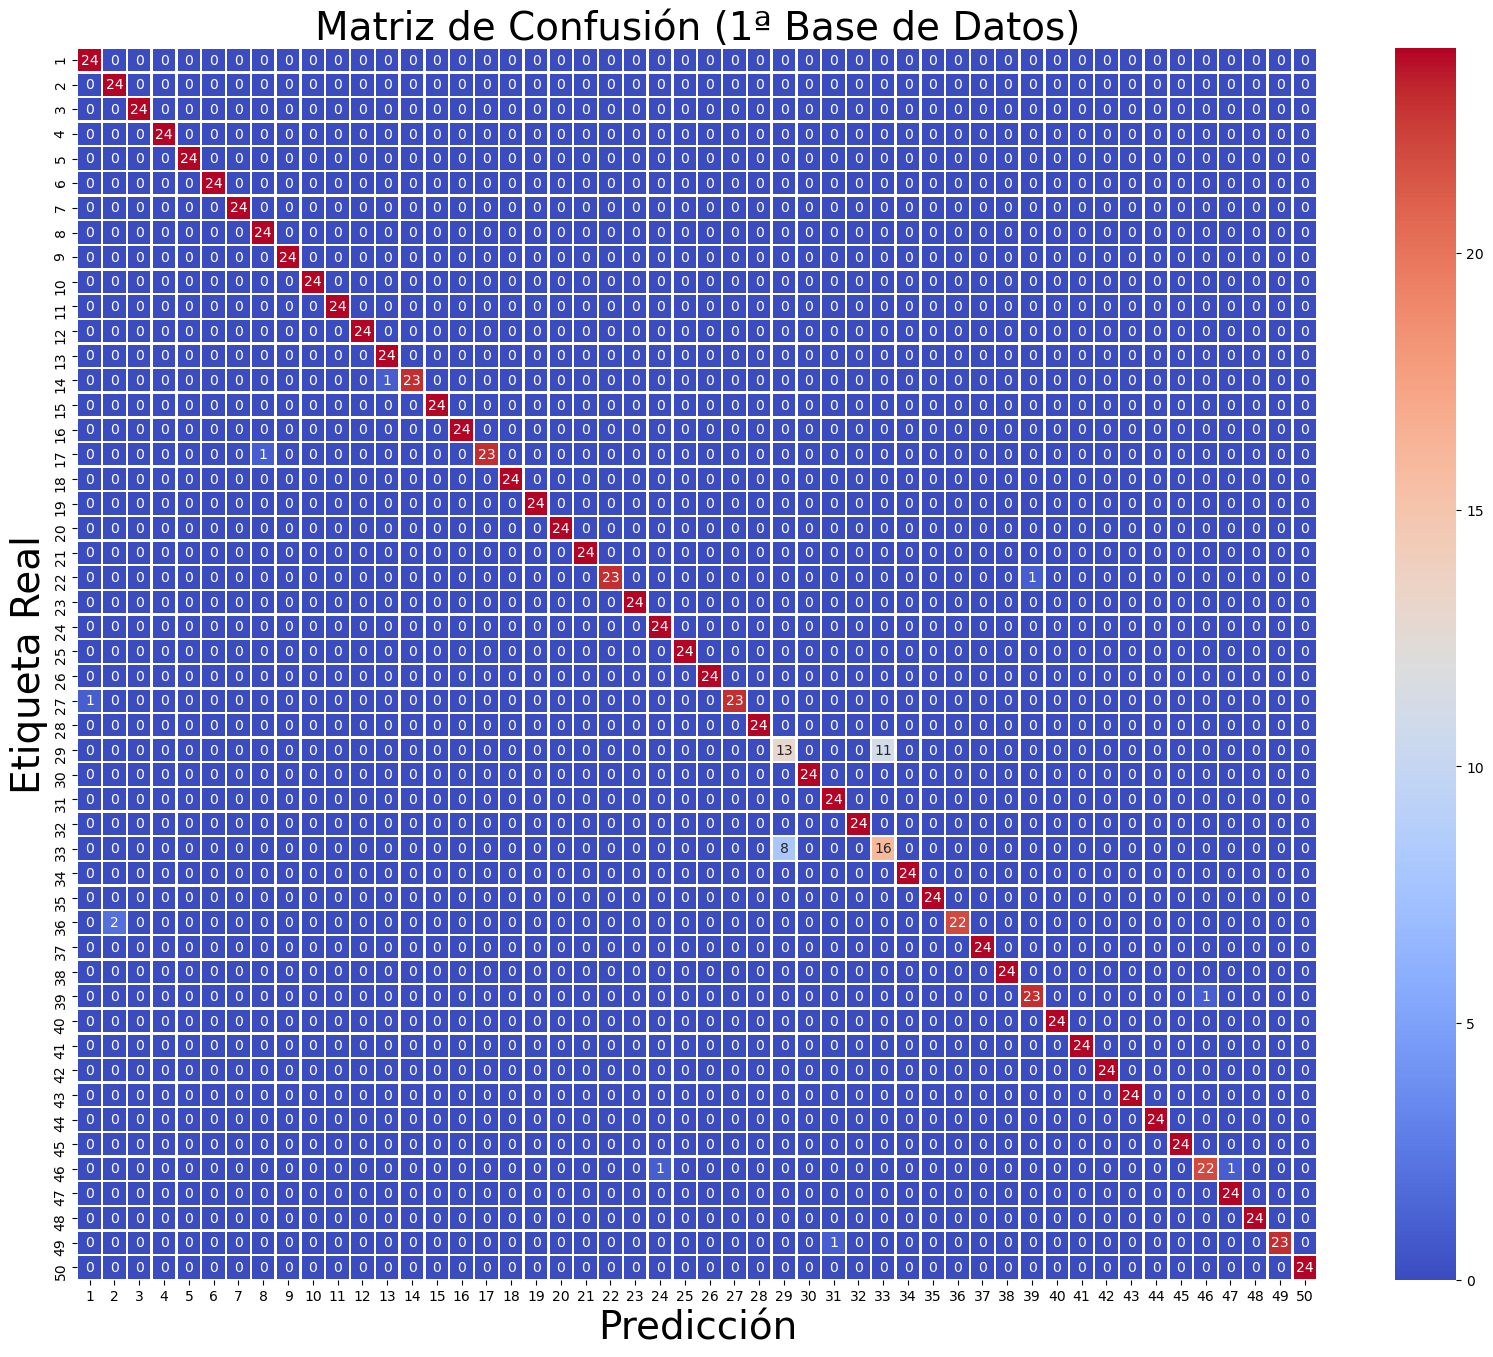
\includegraphics[width=0.7\textwidth]{/cm_1}
	\caption{Matriz de confusi�n obtenida para la base de datos 1.}
	\label{fig:cm1}
\end{figure}

Como se puede ver, es evidente que el sistema no es capaz de  distinguir con tanta precisi�n solo entre los sujetos 29 y 33. Una hip�tesis que cabr�a plantearse es si estas dos personas podr�an tener una relaci�n paterno-filial o fraternal, poniendo en duda la unicidad de la se�al card�aca en ese caso.
%vectores v son bastante diferentes a simple vista, poner�?

La Tabla \ref{rep1} muestra una medici�n de la calidad de las clasificaciones basada en las siguiente m�tricas:
\begin{itemize}
	\item Precisi�n: indica si una predicci�n positiva lo era realmente. \newline
	\begin{center}
		$precision=\frac{VP}{VP + FP}$ %CAMBIAR ESTA FRASE!
	\end{center} 
	\item \textit{Recall} o exhaustividad: indica cu�ntos positivos ha identificado el modelo de todos los posibles positivos.
	\newline
	\begin{center}
		$recall=\frac{VP}{VP + FN}$
	\end{center} 
	\item \textit{F1-score} o valor F: es la media arm�nica entre precisi�n y \textit{recall}. 
	\newline
	\begin{center}
		$F1=2\times\frac{precision\times recall}{precision+recall}$
	\end{center}
\end{itemize}

Siendo $VP$ verdaderos positivos, $FP$ falsos positivos y $FN$ salsos negativos.


Donde \textit{macro avg} es el resultado de calcular las m�tricas de cada etiqueta y obtener su media no ponderada, sin tener en cuenta el desequilibrio entre etiquetas, mientras que en \textit{weighted avg} se obtiene la media ponderada \cite{skit}. 

\begin{table}[h]
	\centering
	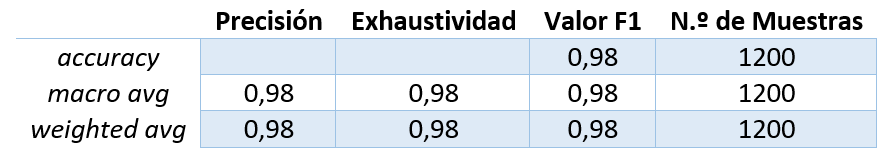
\includegraphics[width=0.8\textwidth]{/report1_2_}
	\caption{Calidad de las clasificaciones obtenidas para la base de datos 1.}
	\label{rep1}
\end{table}


En este caso, para cada usuario se ha utilizado el mismo n�mero de muestras en la evaluaci�n, y estos valores pr�ximos a 1 para las diferentes m�tricas muestran una buena calidad de los resultados. Los valores de cada m�trica para la identificaci�n de cada usuario pueden verse en \ref{clasif1}. Si nos fijamos en los valores obtenidos para los usuarios 29 y 33 nos damos cuenta que, efectivamente, estos son notablemente inferiores que para el resto de usuarios, con un Valor de F1 igual a 0,68 y 0,58 respectivamente. 

Atendiendo a la norma \textit{ISO/IEC JTC 1/SC 37} \cite{iso} y a \textit{Biometrics Evaluation and Testing (BEAT)} \cite{cmcscores, Poh2012}, la m�trica para evaluar un sistema de identificaci�n \textit{closed set} es la curva CMC (\textit{Cumulative Match Characteristic}). En identificaci�n, \textit{$rank(k)$} es el menor valor de $k$ para el cual un identificador correcto de un usuario est� entre los principales $k$ identificadores devueltos por el sistema, y su valor var�a entre 1 y el n�mero de sujetos (en este caso 50). La curva CMC representa gr�ficamente los resultados de test, representando en el eje $x$ los valores de \textit{$rank(k)$}, frente a la probabilidad de que la  identificaci�n sea correcta en ese \textit{rank}, en el eje $y$ \cite{rank}.



\begin{figure}[H]
	\centering
	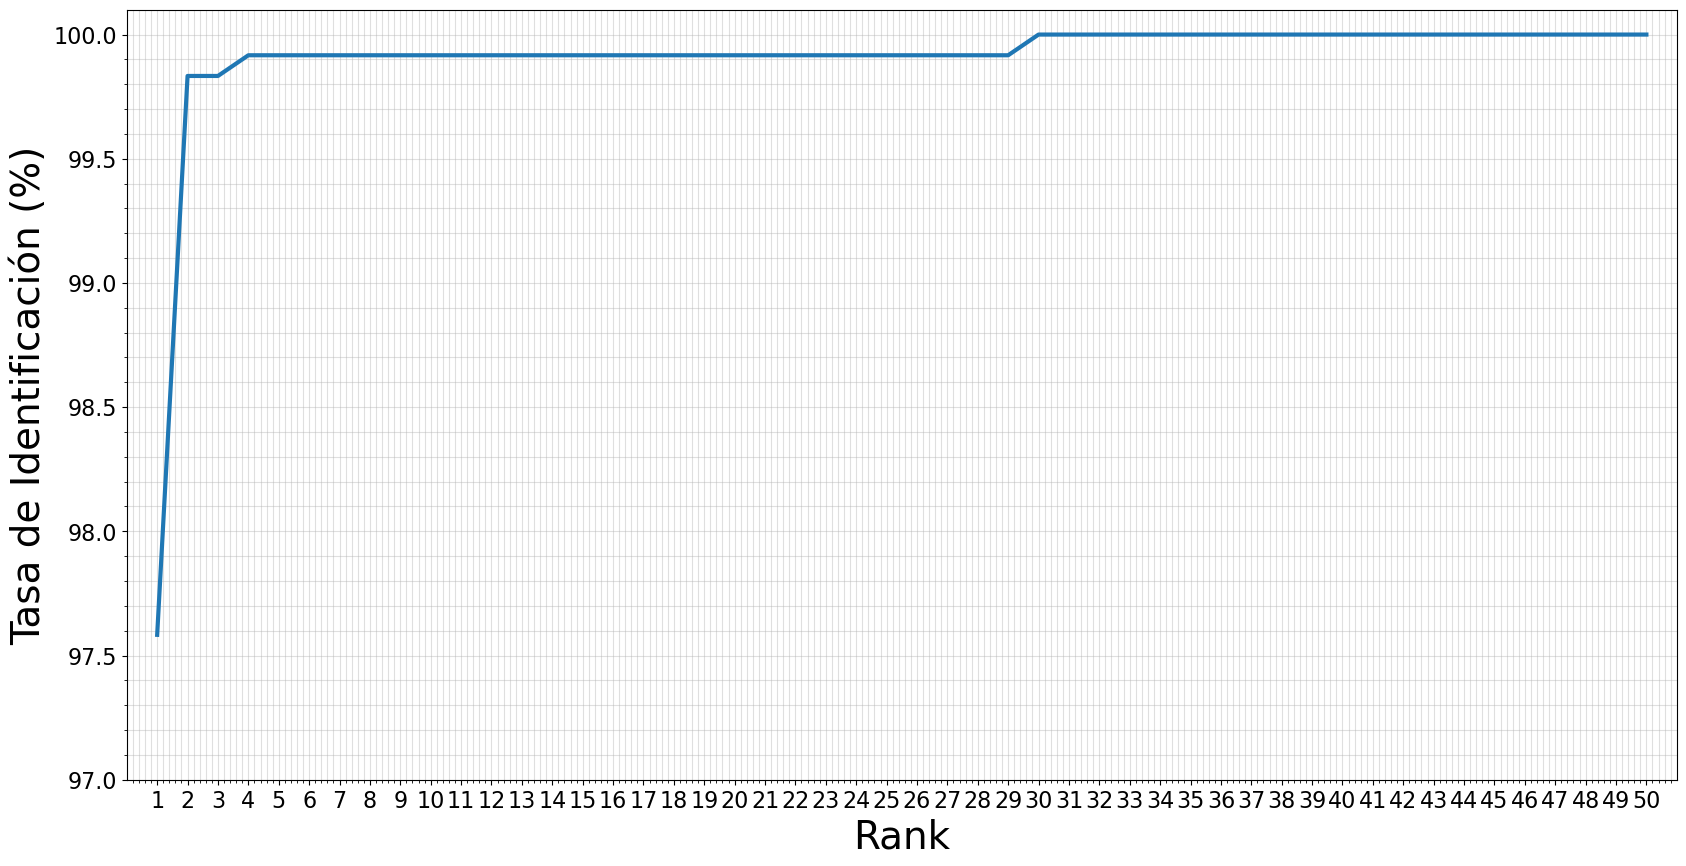
\includegraphics[width=1\textwidth]{/cmc_1}
	\caption{Curva CMC obtenida para los datos de prueba de la base de datos 1.}
	\label{fig:cmc1}
\end{figure}

Como se puede ver, para este modelo hay un primer fallo de identificaci�n en el \break$\textit{rank} = 30$ %checkear que sea 30
, lo que indica que el identificador correcto ten�a por delante 30 identificadores con una mayor probabilidad. Los dem�s fallos en la predicci�n de identidades los encontramos a partir del $\textit{rank} = 4$, dando lugar a una curva muy pr�xima a la esquina superior izquierda. Teniendo en cuenta que un sistema es mejor cuanto m�s se acerca a la esquina superior izquierda \cite{Poh2012}, podemos asegurar que el rendimiento de este sistema es muy prometedor.

 
 %En otros modelos obtenidos en este trabajo con una peor \textit{accuracy}, la CMC ha sido mejor (ver ANEXO). 

%Adem�s, para comprobar la variabilidad intra-sesiones, entrenamiento con muestras una sesi�n y test de la otra sesion. para poder comparar, red entrenada al 50-50

 
\subsection{Segunda base de datos}

Para la segunda base de datos se ha seguido el mismo procedimiento que para la primera, obteniendo %para una divisi�n de los datos $80\%-20\%$, 
resultados de 96,98\%
de rendimiento y 0,13 de p�rdida. Estos resultados se han obtenido utilizando las muestras de ambas sesiones, es decir, incluyendo tomas en reposo y tras realizar ejercicio. 

Adem�s, como las tomas en las que el usuario ha realizado ejercicio son solo un cuarto del total de las tomas, estas han sido a su vez divididas durante el preprocesado en dos nuevas tomas, atendiendo al incremento en el n�mero de QRS presentes en ellas. Con esta modificaci�n de la base de datos se ha vuelto a entrenar una CNN, consiguiendo mejorar el resultado a un 97,39\% de rendimiento y 0,12 de p�rdida.
Estos valores permiten demostrar que la red es capaz de identificar usuarios a�n cuando las muestras incluyen tomas despu�s de haber realizado deporte. 

Las siguientes Figuras y Tablas muestran la matriz de confusi�n, la medici�n de la calidad del clasificador y la curva CMC de este modelo, tal y como se ha hecho para la primera base de datos.

\begin{figure}[H]
	\centering
	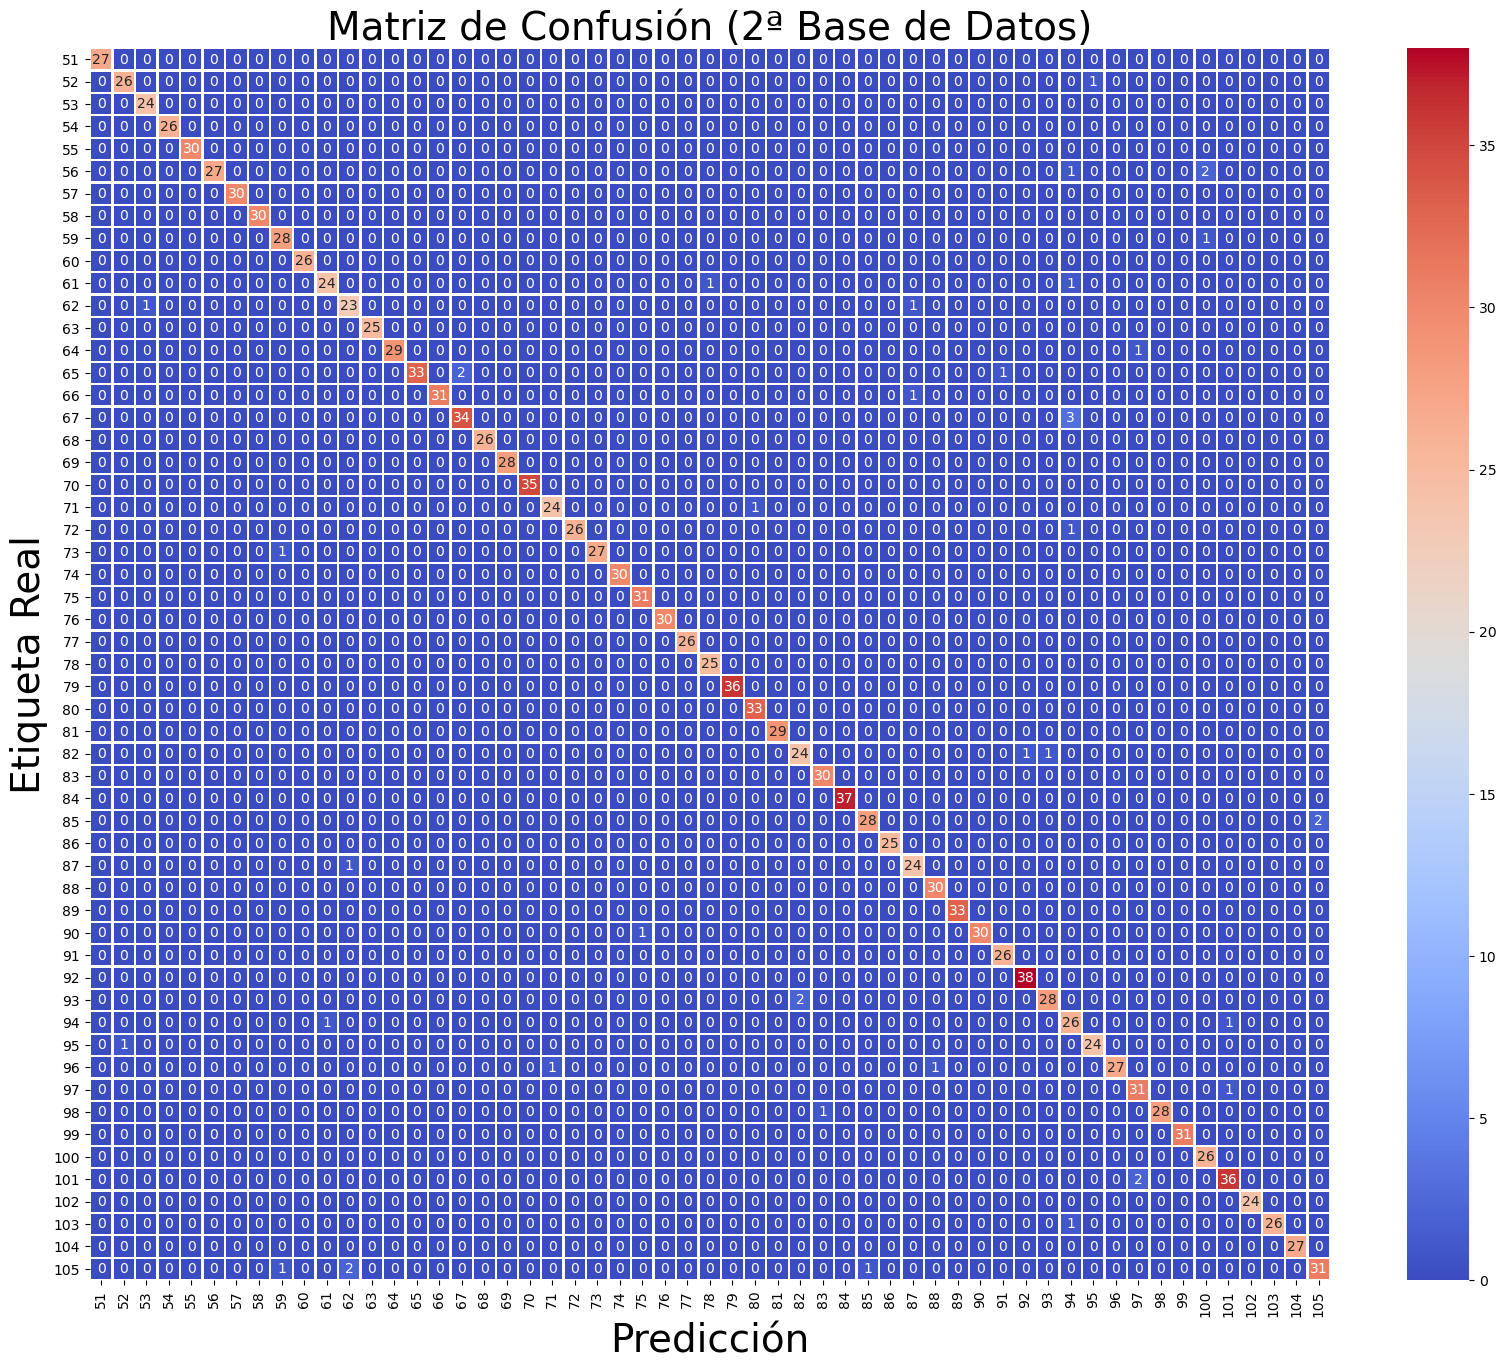
\includegraphics[width=0.7\textwidth]{/cm_2}
	\caption{Matriz de confusi�n obtenida para la base de datos 2.}
	\label{fig:cm2}
\end{figure}

Esta matriz de confusi�n muestra unos muy buenos resultados de predicci�n para todos los usuarios por igual. En este caso, como se puede observar, no se ha utilizado el mismo n�mero de muestras para cada usuario. 

\begin{table}[H]
	\centering
	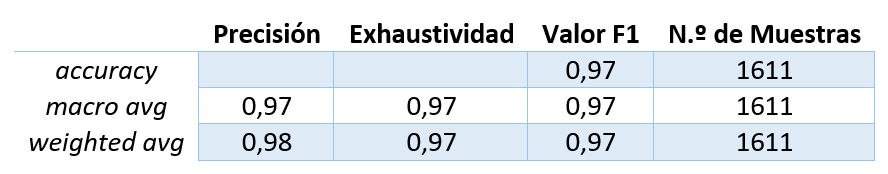
\includegraphics[width=0.8\textwidth]{/report2_2_}
	\caption{Calidad de las clasificaciones obtenidas para la base de datos 2.}
	\label{rep2}
\end{table}


Los resultados de las m�tricas de la identificaci�n de cada usuario por separado se pueden ver en \ref{clasif2}. Como se puede apreciar, en este caso s� hay una ligera diferencia entre la media ponderada y sin ponderar de la precisi�n debido al desequilibrio entre el n�mero de muestras de cada usuario utilizado. 


\begin{figure}[H]
	\centering
	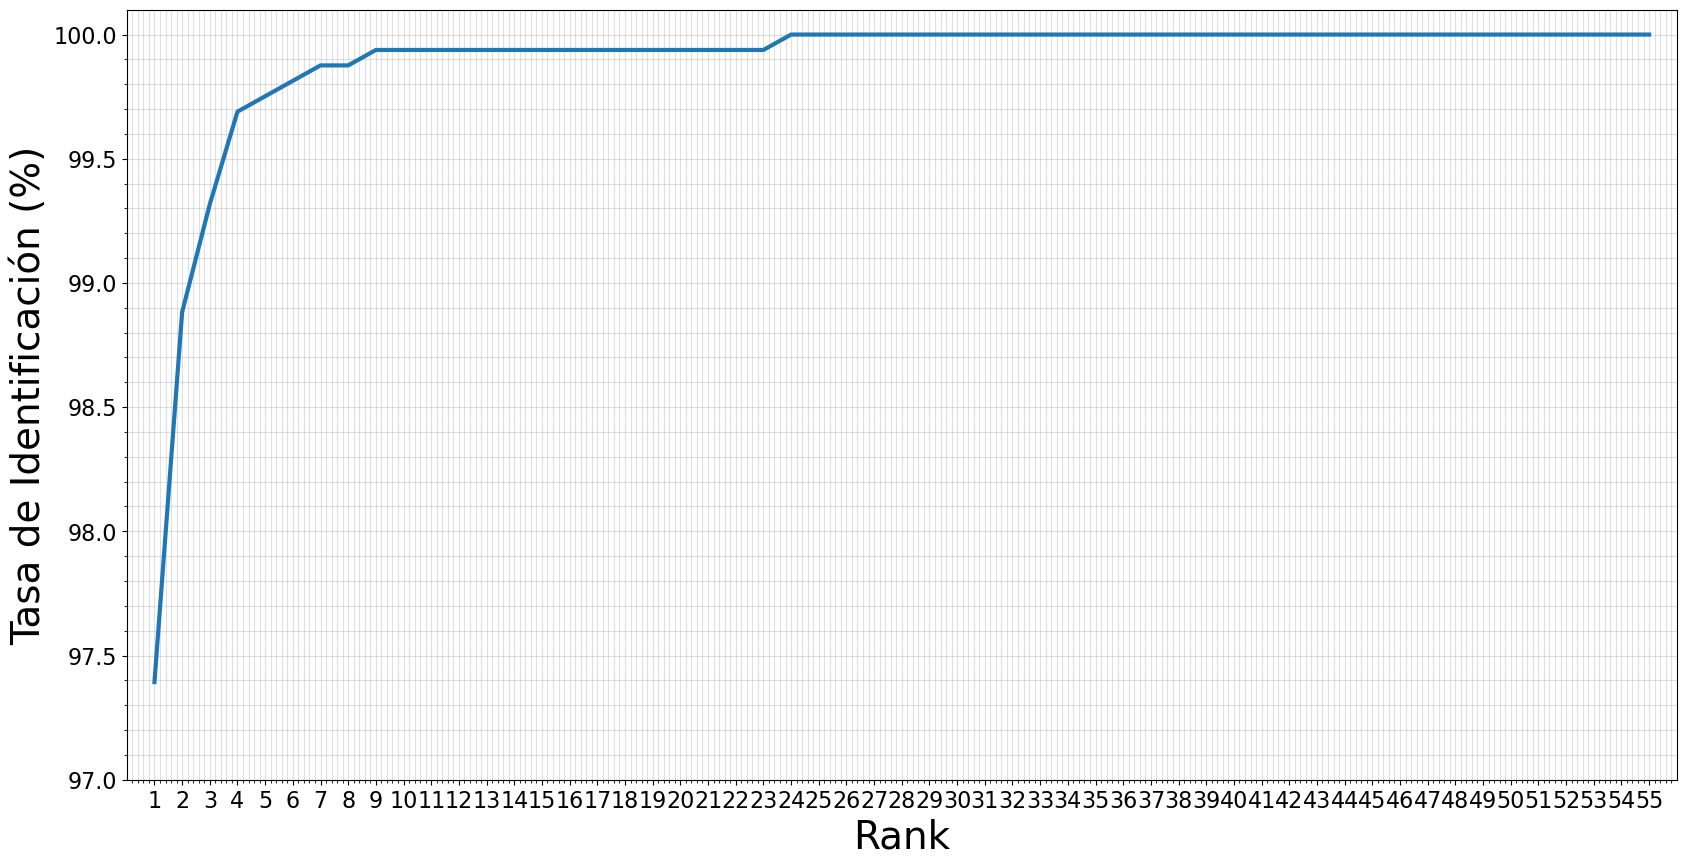
\includegraphics[width=1\textwidth]{/cmc_2}
	\caption{Curva CMC obtenida para la base de datos 2.}
	\label{fig:cmc2}
\end{figure} 

Para este modelo, la curva CMC muestra un primer fallo de identificaci�n en el $\textit{rank} = 24$. Comparando las dos curvas CMC obtenidas (Figura \ref{fig:cmctodas}), podemos ver c�mo a partir del $\textit{rank} = 9$ el rendimiento de este sistema es algo peor que el del primero. A�n as�, se puede considerar que se ha obtenido una buena curva CMC.

%COMPARAR TAMBI�N CON DEEP ECG LA CMC???? 

Como se puede ver, los resultados obtenidos son muy parecidos para ambas bases de datos, lo que demuestra que el ECG se puede utilizar para la identificaci�n de usuarios a�n cuando se incluyen muestras registradas despu�s de haber realizado ejercicio, con un incremento notable del ritmo card�aco. 

\subsection{Base de datos completa}

Tambi�n se ha entrenado una red para toda la base de datos, incluyendo los 105 usuarios, obteniendo un rendimiento de 95,59\% y una p�rdida de 0,18. 

La matriz de confusi�n de este modelo se puede ver en la Figura \ref{fig:cm_}. Si nos fijamos bien, es posible observar como este modelo sigue sin ser capaz de distinguir con precisi�n entre los usuarios 29 y 33. Por otro lado, a diferencia del modelo anterior, este nuevo modelo no es capaz de identificar con tanta precisi�n las muestras del usuario 82, confundiendo a menudo su identidad con la del usuario 93, pero no del rev�s. 

\begin{figure}[H]
	\centering
	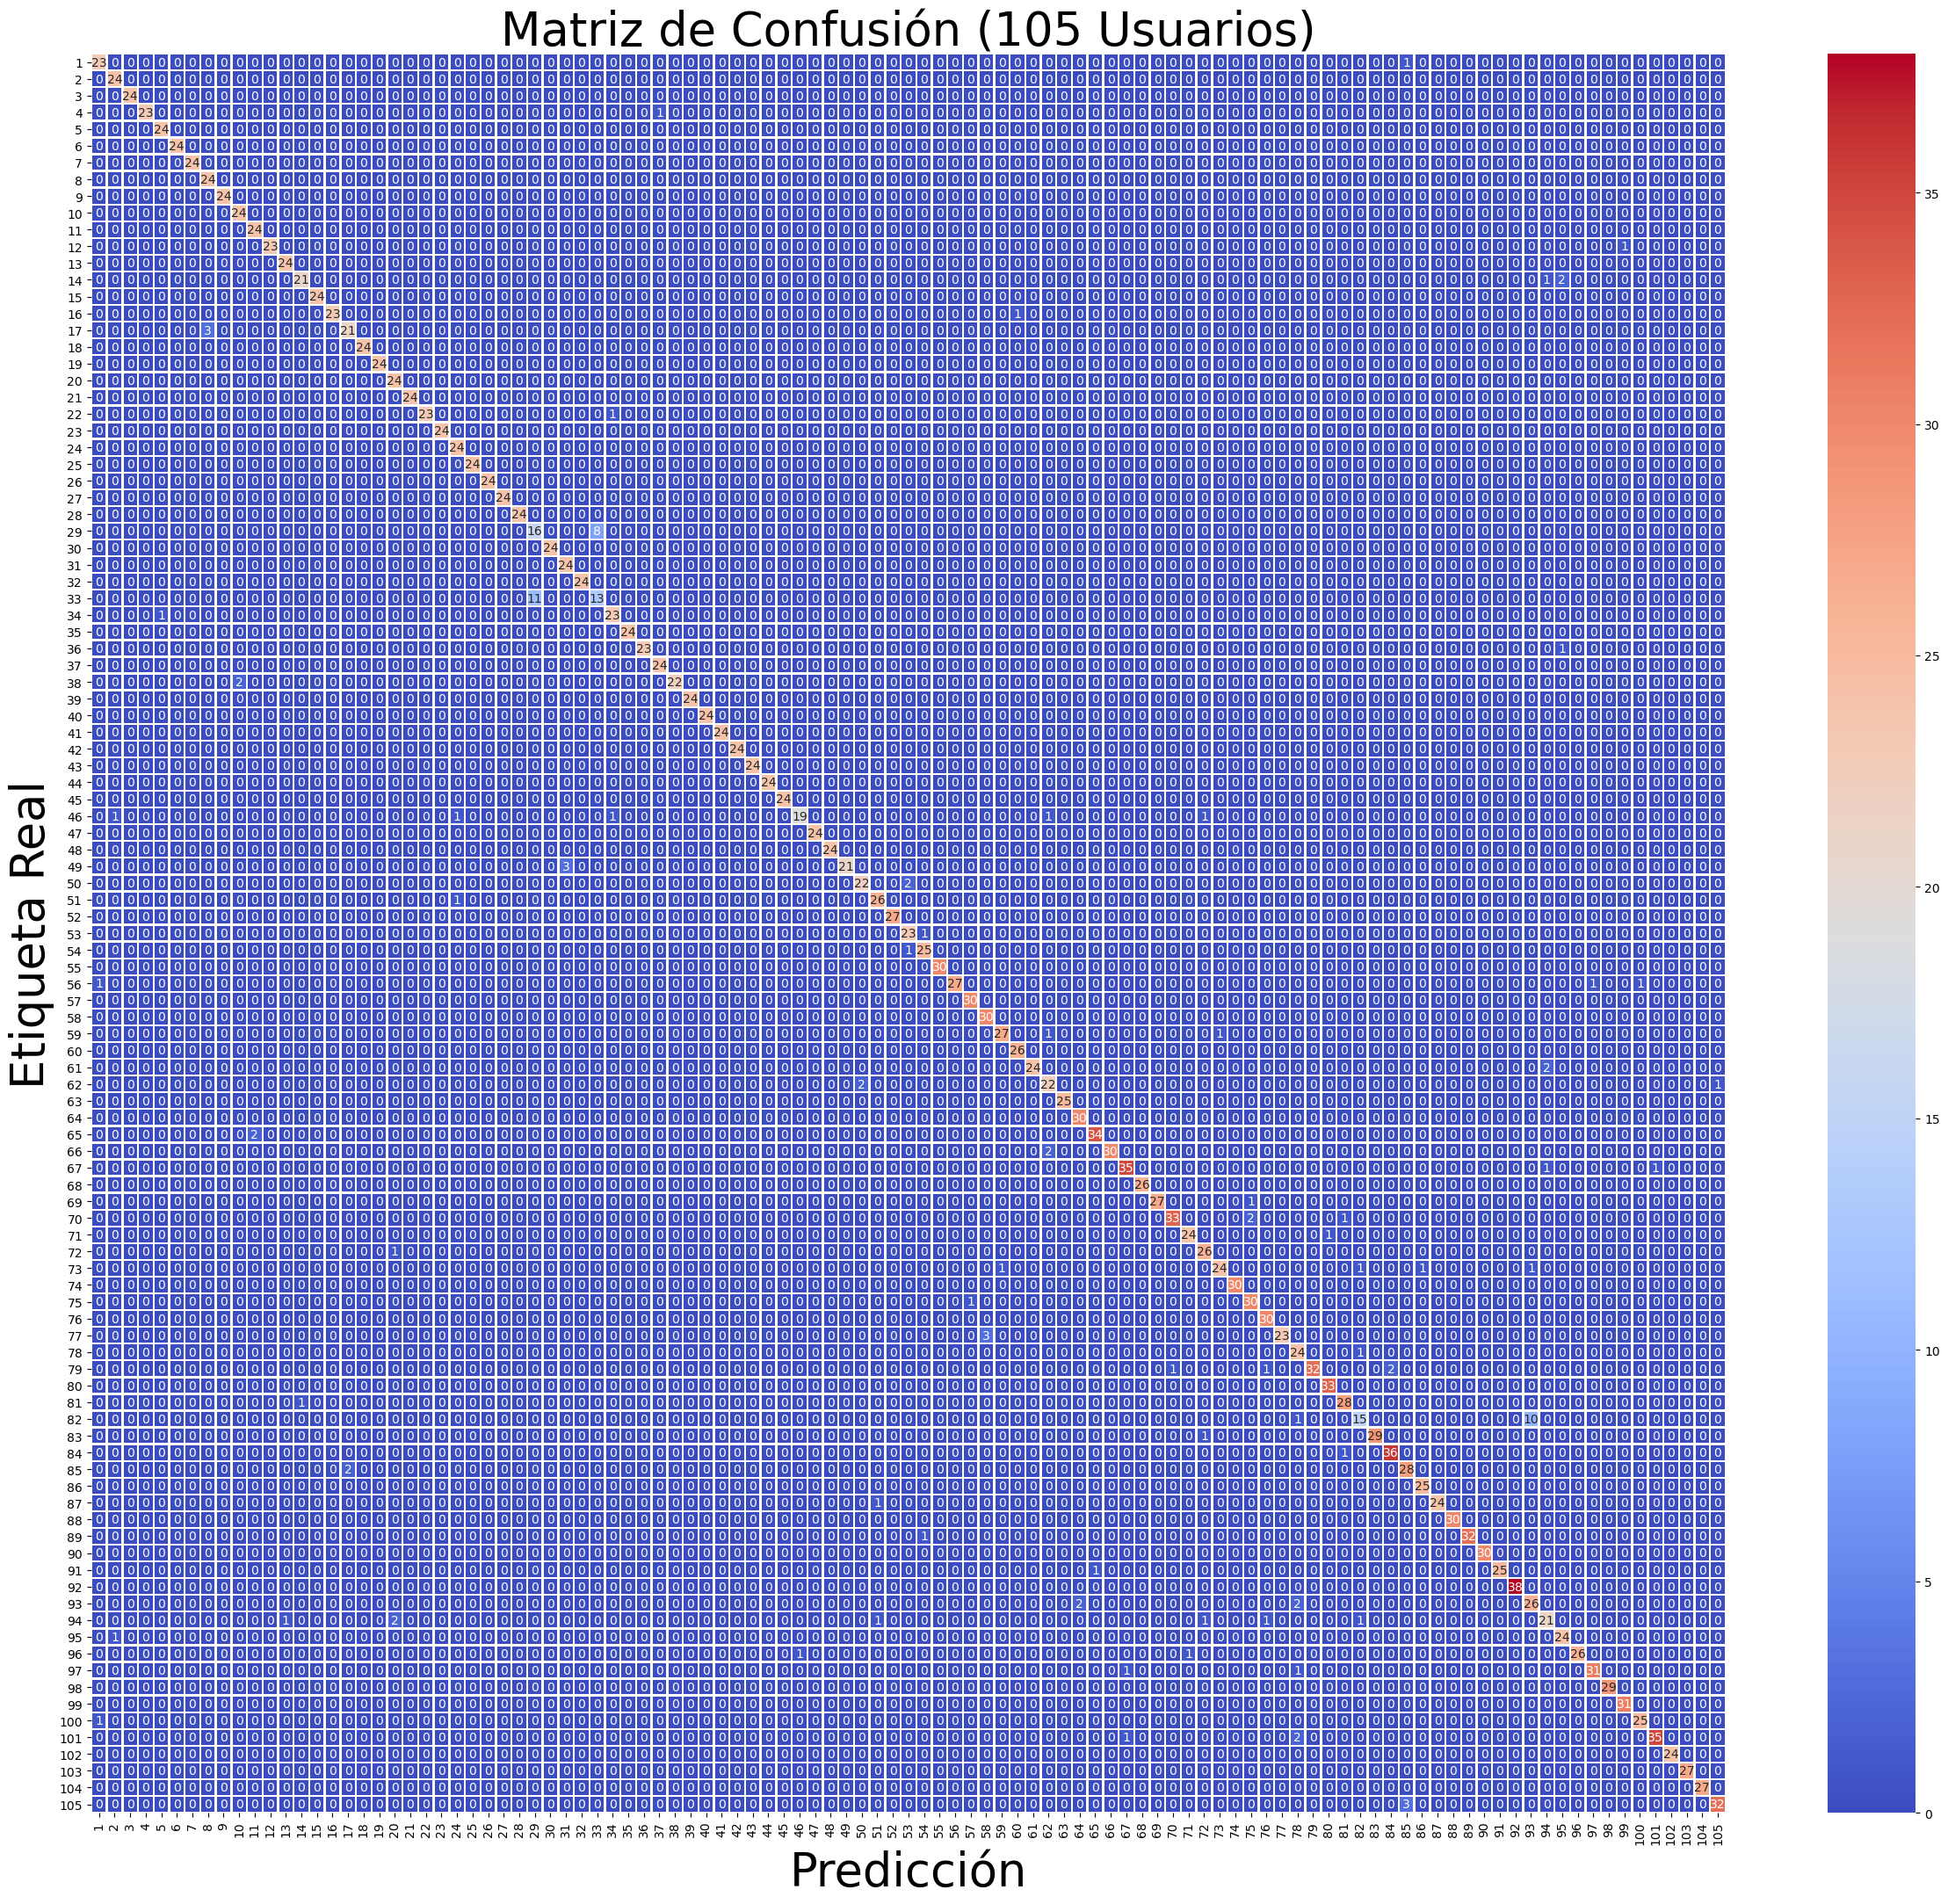
\includegraphics[width=0.9\textwidth]{/cm_}
	\caption{Matriz de confusi�n obtenida para los datos de prueba de la base de datos completa.}
	\label{fig:cm_}
\end{figure}

La m�tricas obtenidas en la evaluaci�n de la calidad del sistema se pueden ver en \ref{appe:A3}. 

La curva CMC obtenida para esta base de datos, comparada con las curvas obtenidas para las otras dos bases de datos, puede verse en la Figura \ref{fig:cmctodas}. Aunque el rendimiento de este modelo sea algo peor, se puede apreciar una buena curva CMC, pr�xima a la obtenida para el modelo que identifica solo a la segunda base de datos.

\begin{figure}[H]
	\centering
	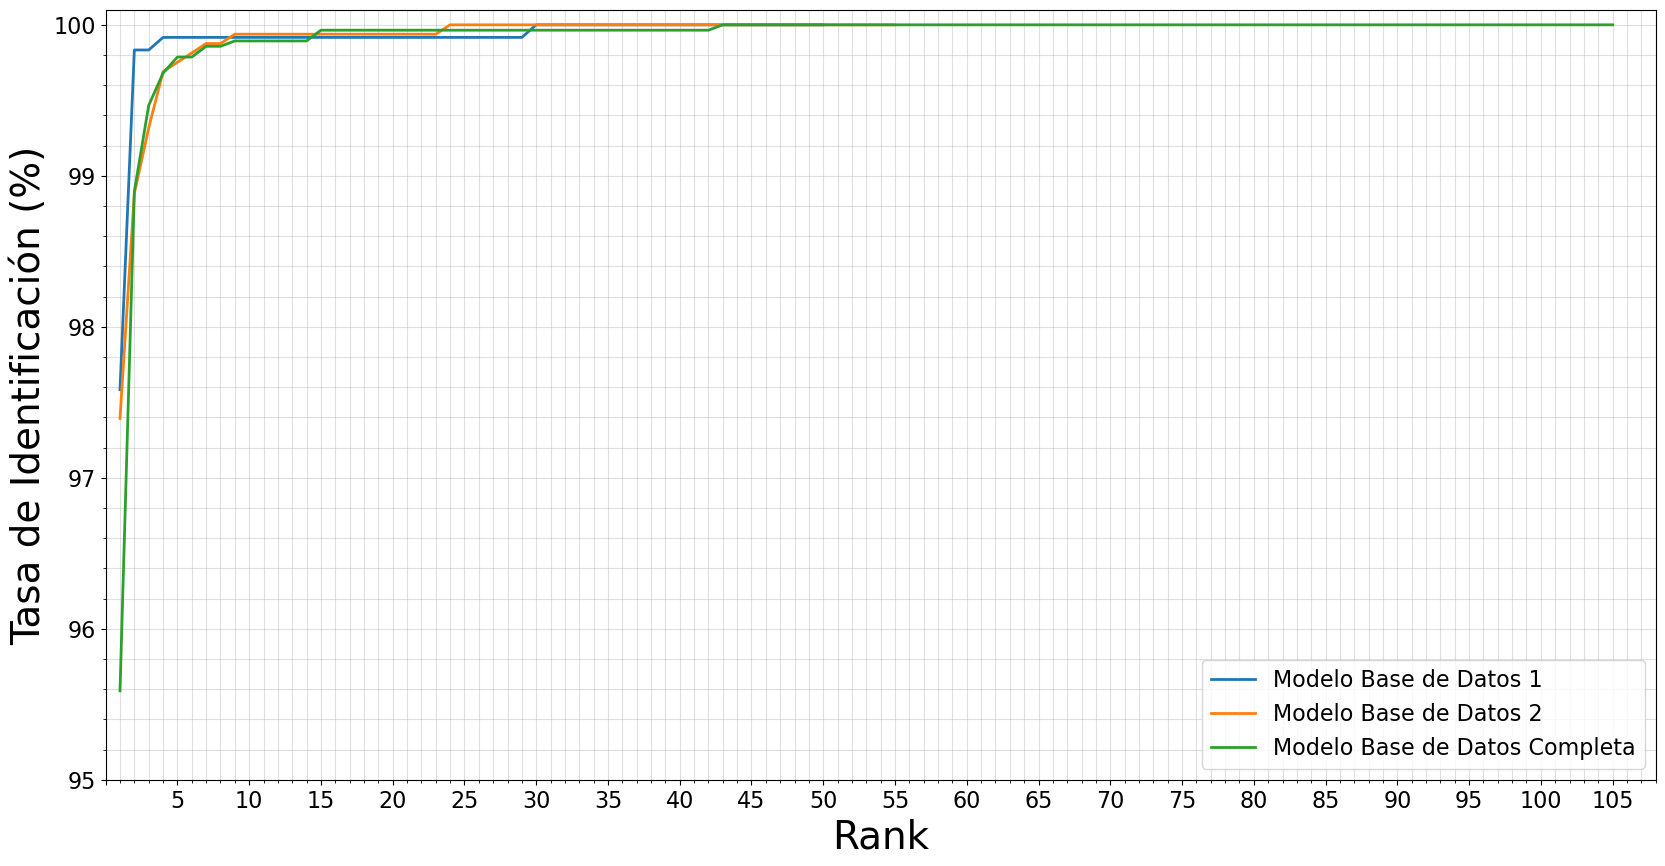
\includegraphics[width=1\textwidth]{/cmc_todas}
	\caption{Comparaci�n de las CMC obtenidas para las bases de datos 1 y 2, as� como la base de datos al completo.}
	\label{fig:cmctodas}
\end{figure} 
%Los dem�s resultados obtenidos se pueden observar a continuaci�n/ en el anexo (DECIDIR). 
 
 Adem�s, la siguiente Figura (\ref{todo}) muestra una comparativa de la tasa de identificaci�n para el \textit{rank(1)} en funci�n del n�mero de usuarios registrados en el sistema. Cabe recordar que ninguno de los usuarios utilizados para los valores de 50 y 55  son los mismos, mientras que el valor 105 corresponde a la uni�n de ambos. 
 
\begin{figure}[H]
	\centering
	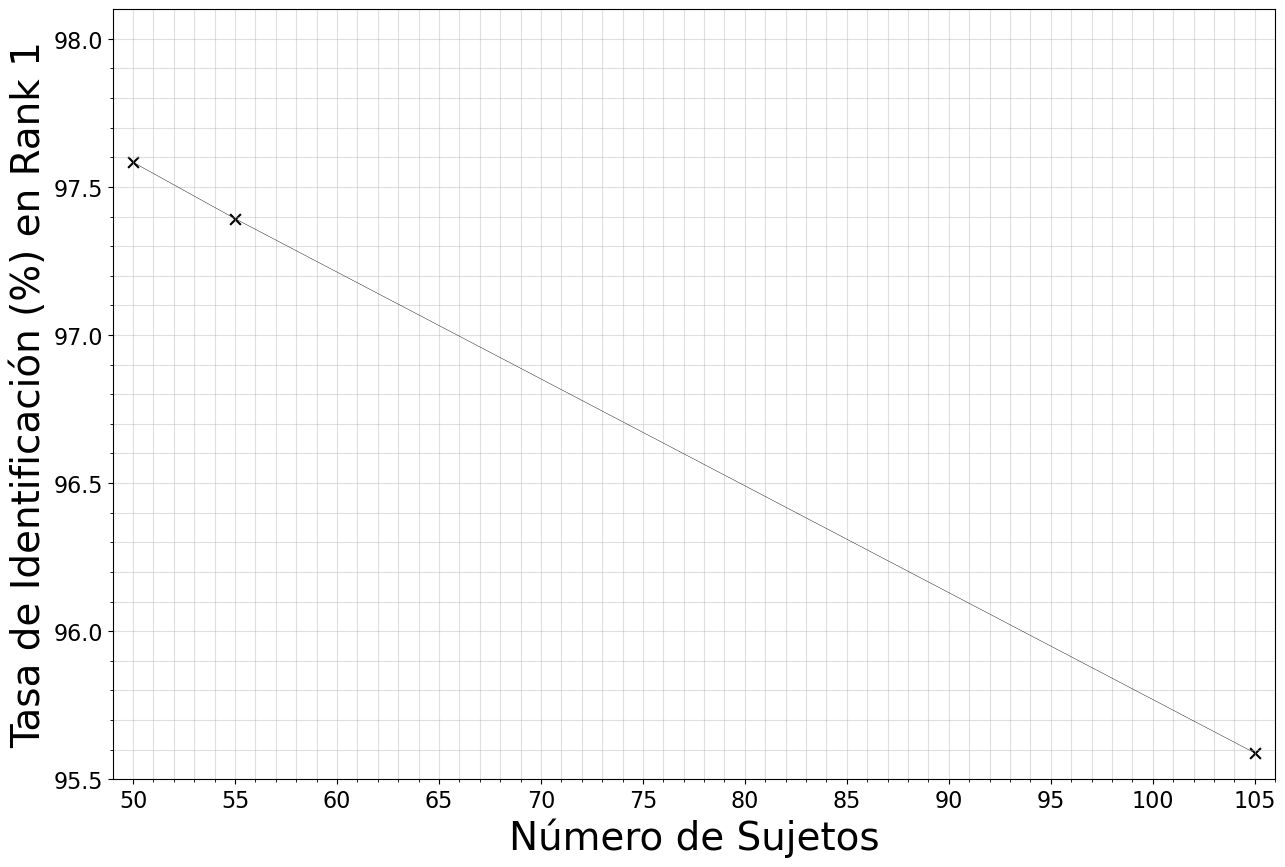
\includegraphics[width=0.7\textwidth]{/rank1}
	\caption{Variaci�n de la tasa de identificaci�n en el rank(1) en funci�n del n�mero de sujetos.}
	\label{todo}
\end{figure}
 
 Como se puede ver, en este caso la identificaci�n ha empeorado cuando ha aumentado el n�mero de usuarios registrados. Sin embargo, ajustando los hiperpar�metros de red de este �ltimo modelo, probablemente se podr�an llegar a conseguir mejores resultados. 
 
\subsection{Variabilidad intra-clase}

Por �ltimo, se ha querido comprobar la estabilidad del ECG como caracter�stica biom�trica. Para ello, se ha utilizado solo la primera base de datos, entrenando una red con los registros de la primera sesi�n y evaluando el sistema con los registros de la segunda sesi�n, y viceversa. Por tanto, la divisi�n de muestras en esta configuraci�n ha sido $50\%$ de entrenamiento y $50\%$ de test. Para poder comparar los resultados con los obtenidos cuando las muestras de ambas sesiones est�n mezcladas, se ha entrenado tambi�n otra red con una divisi�n $50-50\%$. Los resultados obtenidos han sido los siguientes (Tabla \ref{ses}):

\begin{table}[H]
	\centering
	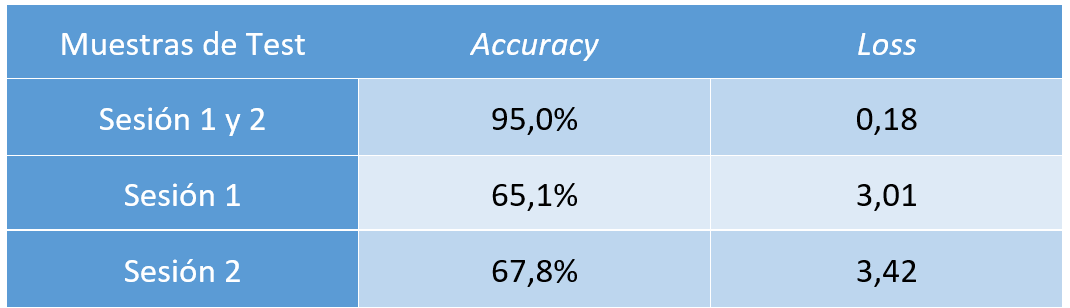
\includegraphics[width=0.8\textwidth]{/interses_2_2}
	\caption{Comparaci�n de los resultados de rendimiento y p�rdida obtenidos con variabilidad intra-clase.}
	\label{ses}
\end{table}


Se puede apreciar que la identificaci�n de usuarios es notablemente peor cuando la evaluaci�n del sistema se realiza con muestras registradas en  un d�a diferente al de las muestras utilizadas para el entrenamiento de la red. Por tanto, no podemos demostrar la estabilidad del ECG como caracter�stica biom�trica con este estudio. 


\section{Autenticaci�n} \label{aut}

El proceso de autenticaci�n se divide (como ya hemos visto) en dos fases: reclutamiento y consulta. Para el reclutamiento se ha utilizado el $80\%$ de las muestras de cada usuario del cual se quiere verificar la identidad, y el $20\%$ restantes se han reservado para realizar las consultas. Por tanto, las muestras de verificaci�n nunca se han utilizado en el reclutamiento, ni viceversa.

Para evaluar el sistema se han realizado pruebas sobre 3 modelos diferentes:
\begin{itemize}
	\item Modelo 1: se verifica la identidad de los 55 usuarios de la segunda base de datos (que recordamos, incluye tomas registradas despu�s de haber realizado ejercicio). Para ello, se utiliza una red entrenada con los 50 usuarios de la primera base de datos, es decir, el porcentaje de usuarios utilizado para el entrenamiento es del $47\%$. 
	\item Modelo 2: se verifica la identidad de los 50 usuarios de la primera base de datos, utilizando una red entrenada con los 55 de la segunda ($54\%$).
	\item Modelo 3: para comprobar la influencia del porcentaje de usuarios utilizados para el entrenamiento, se ha entrenado una nueva red con el $80\%$ de los usuarios totales (84 usuarios) y se ha verificado la identidad del 20\% de usuarios restantes. %Por tanto, en esta configuraci�n, tanto en el entrenamiento como en la autenticaci�n
\end{itemize}



\begin{figure}[H]
	\centering
	\subfigure{
		\label{fig:mod1}
		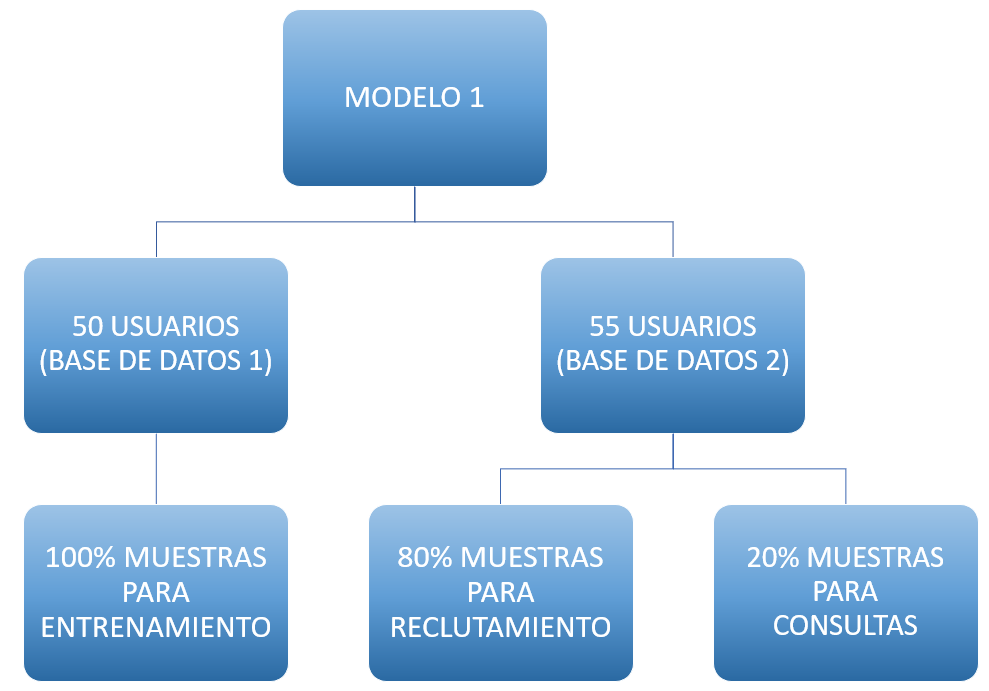
\includegraphics[width=0.45\textwidth]{/modelo1}}
	\hspace{1cm}
	\subfigure{
		\label{fig:mod2}
		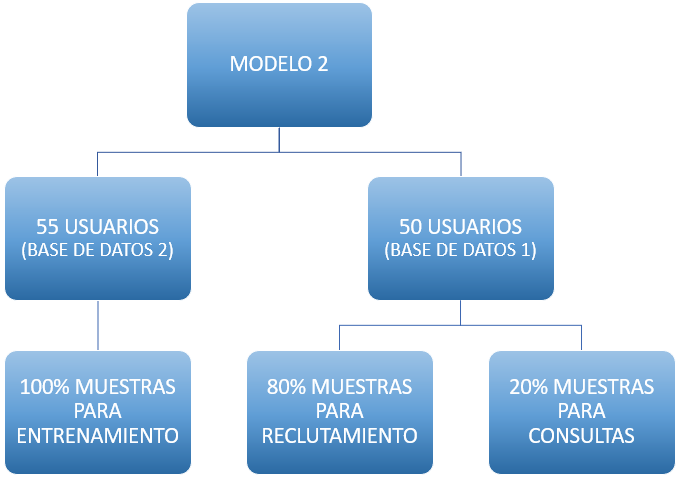
\includegraphics[width=0.45\textwidth]{/modelo2}}
	\subfigure{
		\label{fig:mod3}
		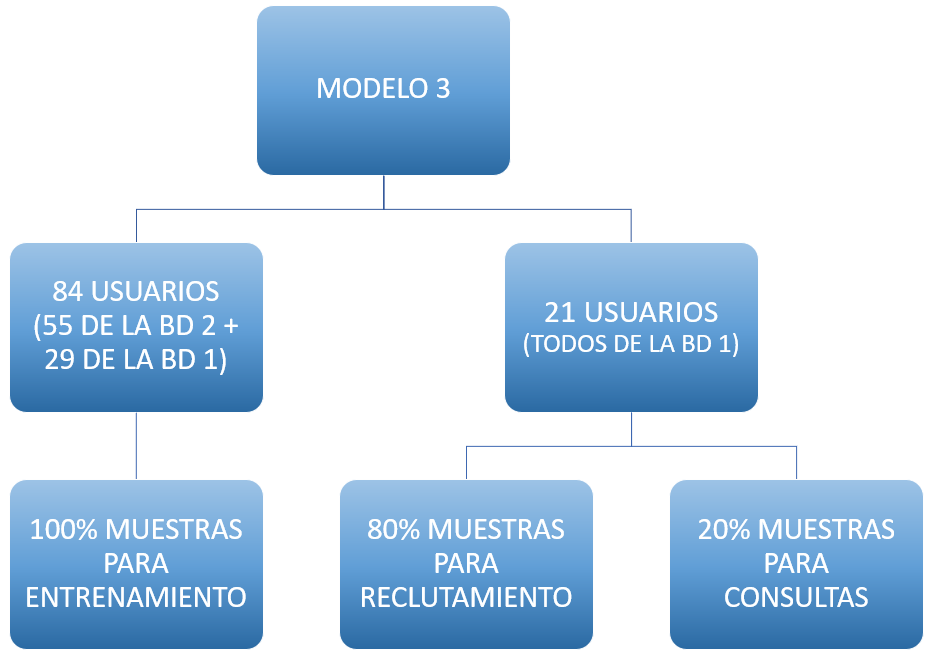
\includegraphics[width=0.45\textwidth]{/modelo3}}
	\caption{Esquema de la divisi�n de usuarios y de sus muestras para las distintas fases en cada modelo.}
	\label{mods}
\end{figure}

Para visualizar los vectores de caracter�sticas obtenidos durante la fase de reclutamiento, se han utilizado las herramientas PCA y TSNE \cite{skit}. Estas herramientas permiten la visualizaci�n de datos de grandes dimensiones, mediante la reducci�n de su dimensionalidad. % (el anexo ref{} incluye una descripci�n m�s detallada de ambos algoritmos).

Como se puede ver en la Figura \ref{tsne}, los vectores de caracter�sticas se encuentran bastante agrupados en el espacio en funci�n del usuario al que corresponden. Estas agrupaciones por usuarios son m�s evidentes en el Modelo 3, pero esto puede deberse a que solo hay 21 usuarios registrados en el sistema y por eso la visualizaci�n es mejor. Entre el Modelo 1 y el 2, cabr�a esperar obtener mejores resultados para el segundo, donde estas agrupaciones est�n m�s definidas. Visualizando de esta manera los vectores de caracter�sticas de cada usuario, es bastante evidente que s� se puede distinguir a las personas a trav�s de su se�al de ECG. En \ref{pca} se puede ver la visualizaci�n de los mismos vectores con la herramienta PCA.


\begin{figure}[H]
	\centering
	\subfigure[MODELO 1]{
		\label{fig:tsne1}
		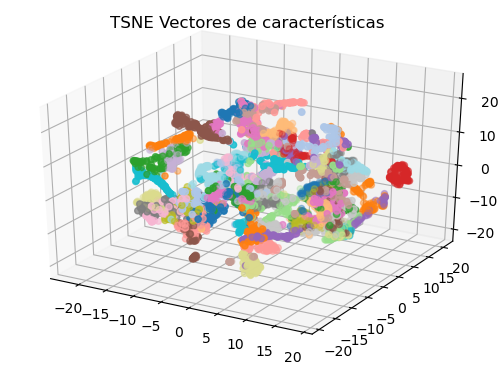
\includegraphics[width=0.45\textwidth]{/tsne1}}
	\subfigure[MODELO 2]{
		\label{fig:tsne2}
		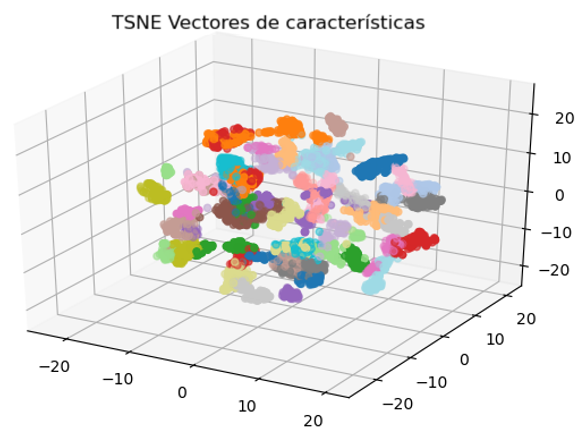
\includegraphics[width=0.45\textwidth]{/tsne2}}
	\subfigure[MODELO 3]{
		\label{fig:tsne3}
		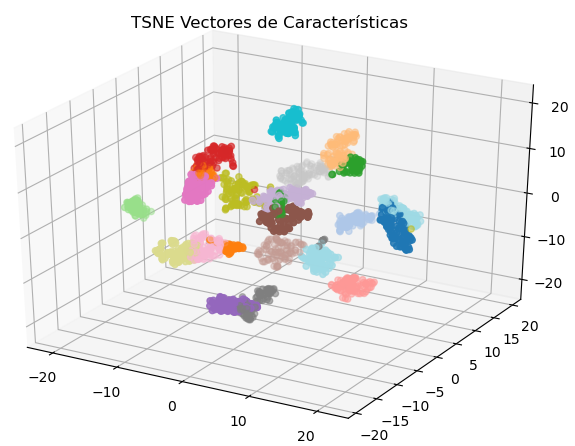
\includegraphics[width=0.45\textwidth]{/tsne3}}
	\caption{Comparativa de la distribuci�n de los vectores de caracter�sticas obtenidos durante la fase de reclutamiento para cada modelo, empleando la herramienta de visualizaci�n TSNE para reducir a tres dimensiones el espacio.}
	\label{tsne}
\end{figure}



Para evaluar el sistema,  con cada muestra de cada usuario se han realizado consultas genuinas, en las que se compara la muestra con su patr�n registrado, pero tambi�n consultas de ``impostores'', donde se compara la muestra de ese usuario con los patrones registrados de todos los dem�s usuarios. Cada consulta, ya sea genuina o no, se considera independiente, luego para \underline{una �nica muestra} hay tantas consultas como usuarios $(n)$ registrados en el sistema, de las cuales solo $1$ es genuina y el resto $(n - 1)$ de impostores. Aunque en un escenario m�s realista para un sistema de autenticaci�n se espera que el n�mero de consultas genuinas sea mayor que el de consultas de impostores, en este estudio se ha utilizado esta metodolog�a para poder evaluar m�s a fondo el rendimiento del sistema con los datos disponibles. 

Como el n�mero de consultas depende del n�mero de usuarios registrados en cada modelo, para llevar a cabo una comparativa entre los mismos se va a hablar siempre del n�mero de muestras \textit{m} por usuario que se ha utilizado para realizar las consultas \textit{q}, con $q = n \times (m \times n)$. 

\begin{figure}[H]
	\centering
	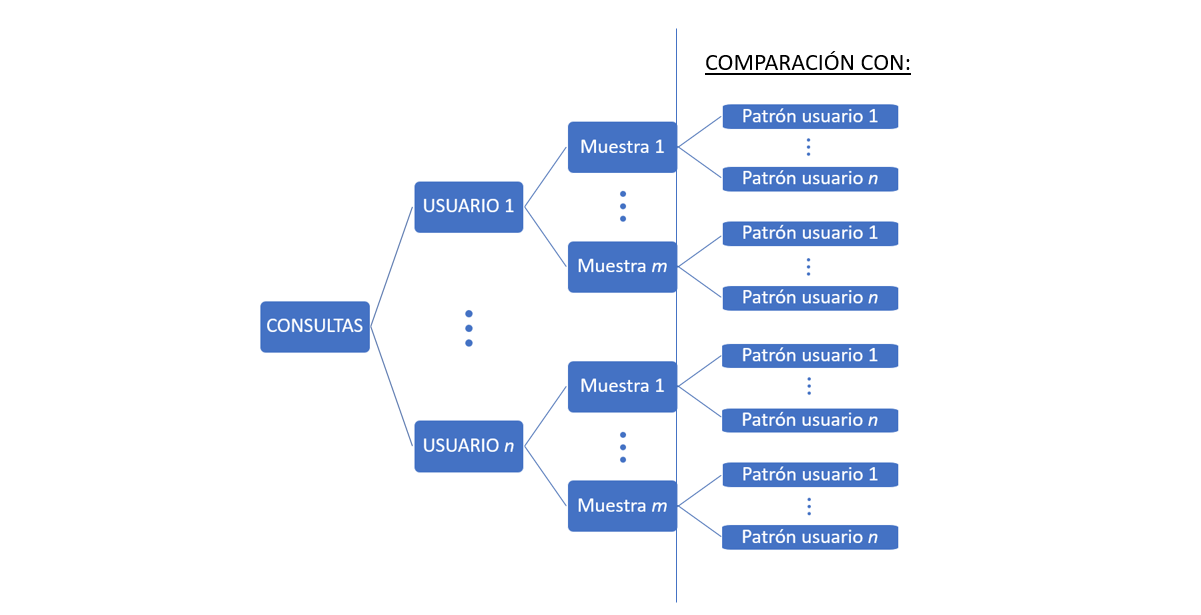
\includegraphics[width=1.1\textwidth]{/consultas2}
	\caption{Esquema de la fase de consulta.}
	\label{consultas}
\end{figure}



La distribuci�n de las distancias euclideas obtenidas al utilizar todas las muestras del set de consulta para realizar con ellas todas las consultas posibles, se puede observar en la Figura \ref{histo}. Como la mayor�a de las consultas son de impostores, esta visualizaci�n de las distancias permite hacerse una idea de d�nde deber�a establecerse el umbral. 
Adem�s, se ve claramente como la mayor�a de distancias se encuentran dentro de un rango de valores, y solo unas pocas (las correspondientes a las consultas genuinas) tienen una distancia menor. Aunque en el modelo en el que mejor se aprecia es en el 3, esto se debe a que al haber menos usuarios registrados el n�mero de consultas realizadas tambi�n es menor (aproximadamente un sexto de las consultas realizadas en los otros 2 modelos). 
Por otro lado, es notable la diferencia del rango de valores obtenidos para las distancias entre los modelos, estando todas las distancias bastante m�s concentradas en el Modelo 2 (entre 2,5 y 37). 

%REPASAR ESTE PARRAFO

\begin{figure}[H]
	\centering
	\subfigure[MODELO 1]{
		\label{fig:histo1}
		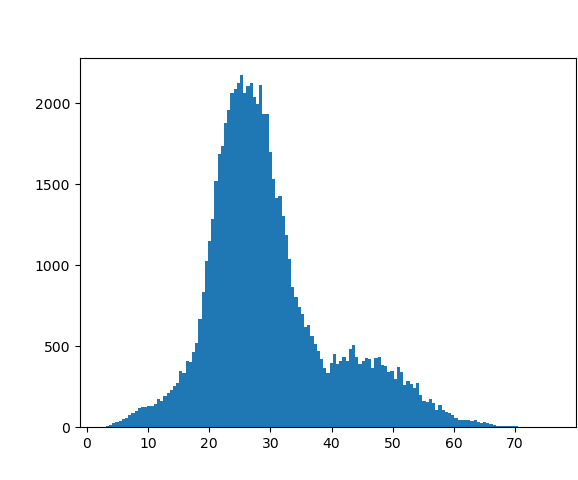
\includegraphics[width=0.3\textwidth]{/histo1_}}
	\subfigure[MODELO 2]{
		\label{fig:histo2}
		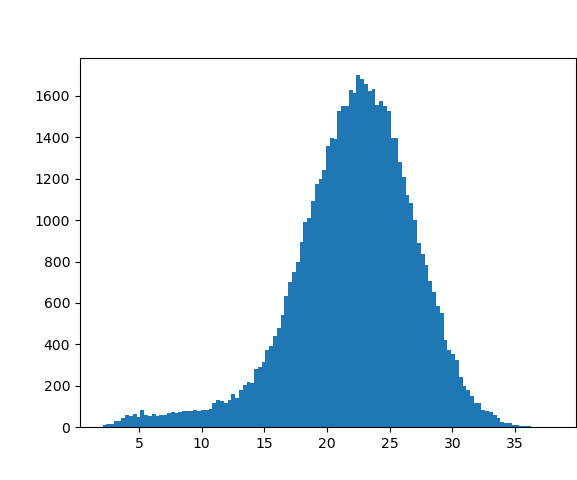
\includegraphics[width=0.3\textwidth]{/histo2_}}
	\subfigure[MODELO 3]{
		\label{fig:histo3}
		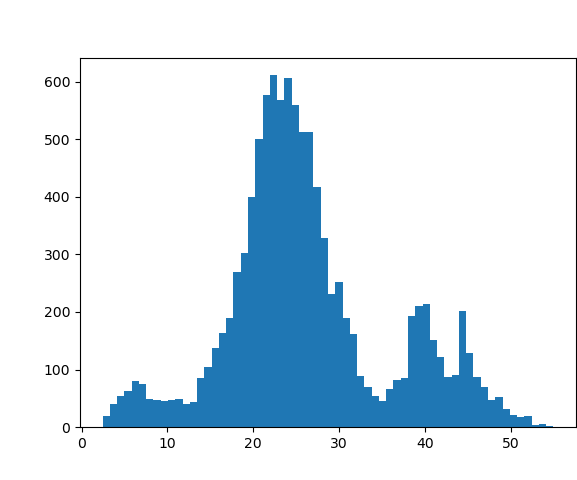
\includegraphics[width=0.3\textwidth]{/histo3_}}
	\caption{Distribuci�n de usuarios genuinos e impostores mediante la distancia eucl�dea.}
	\label{histo}
\end{figure} 

Atendiendo a la norma \textit{ISO/IEC JTC 1/SC 37} \cite{iso} y a \textit{Biometrics Evaluation and Testing (BEAT)} \cite{cmcscores, Poh2012}, las m�tricas utilizadas para evaluar un sistema de autenticaci�n son:

\begin{itemize}
	\item \textit{Failure-to-enrrol rate}: proporci�n de los usuarios para los que el sistema no ha completado la fase de reclutamiento.
	\item \textit{Failure-to-acquire rate}: proporci�n de intentos de verificaci�n o identificaci�n en los que el sistema no logra captar o localizar una imagen o se�al de calidad suficiente. 
	\item Tasa de Falsa Aceptaci�n o FAR (de sus siglas en ingl�s): proporci�n de intentos de acceso no autorizados aceptados incorrectamente por el sistema.		
	\item Tasa de Falso Reconocimiento o FRR (de sus siglas en ingl�s): proporci�n de intentos de acceso autorizados denegados incorrectamente por el sistema.
\end{itemize}

%PONER LAS FORMULAS DEL FAR Y FRR BIEN 
En este trabajo, la tasa de adquisici�n se desconoce y la tasa de error de enrolamiento no se ha tenido en cuenta, por lo que se considera tambi�n como desconocida.  \\El FAR y el FRR han sido calculados de la siguiente manera:
\begin{center}
$FAR =  \frac{\textup{Falsos Positivos}}{\textup{N� Total de Consultas}}$  

$FRR = \frac{Falsos Negativos}{N� Total de Consultas}$

\end{center} 
%como la proporci�n de falsos positivos $(FP)$ y falsos negativos $(FN)$ sobre el total de comparaciones realizadas $(VP + FP + VN + FN)$, respectivamente. 
Adem�s, la m�trica empleada para comparar el rendimiento de los diferentes modelos ha sido el \textit{Equal Error Rate} (EER), que se obtiene variando el umbral y representando gr�ficamente las curvas FAR y FRR obtenidas, siendo el EER el punto de intersecci�n entre ambas. 



\begin{figure}[H]
	\centering
	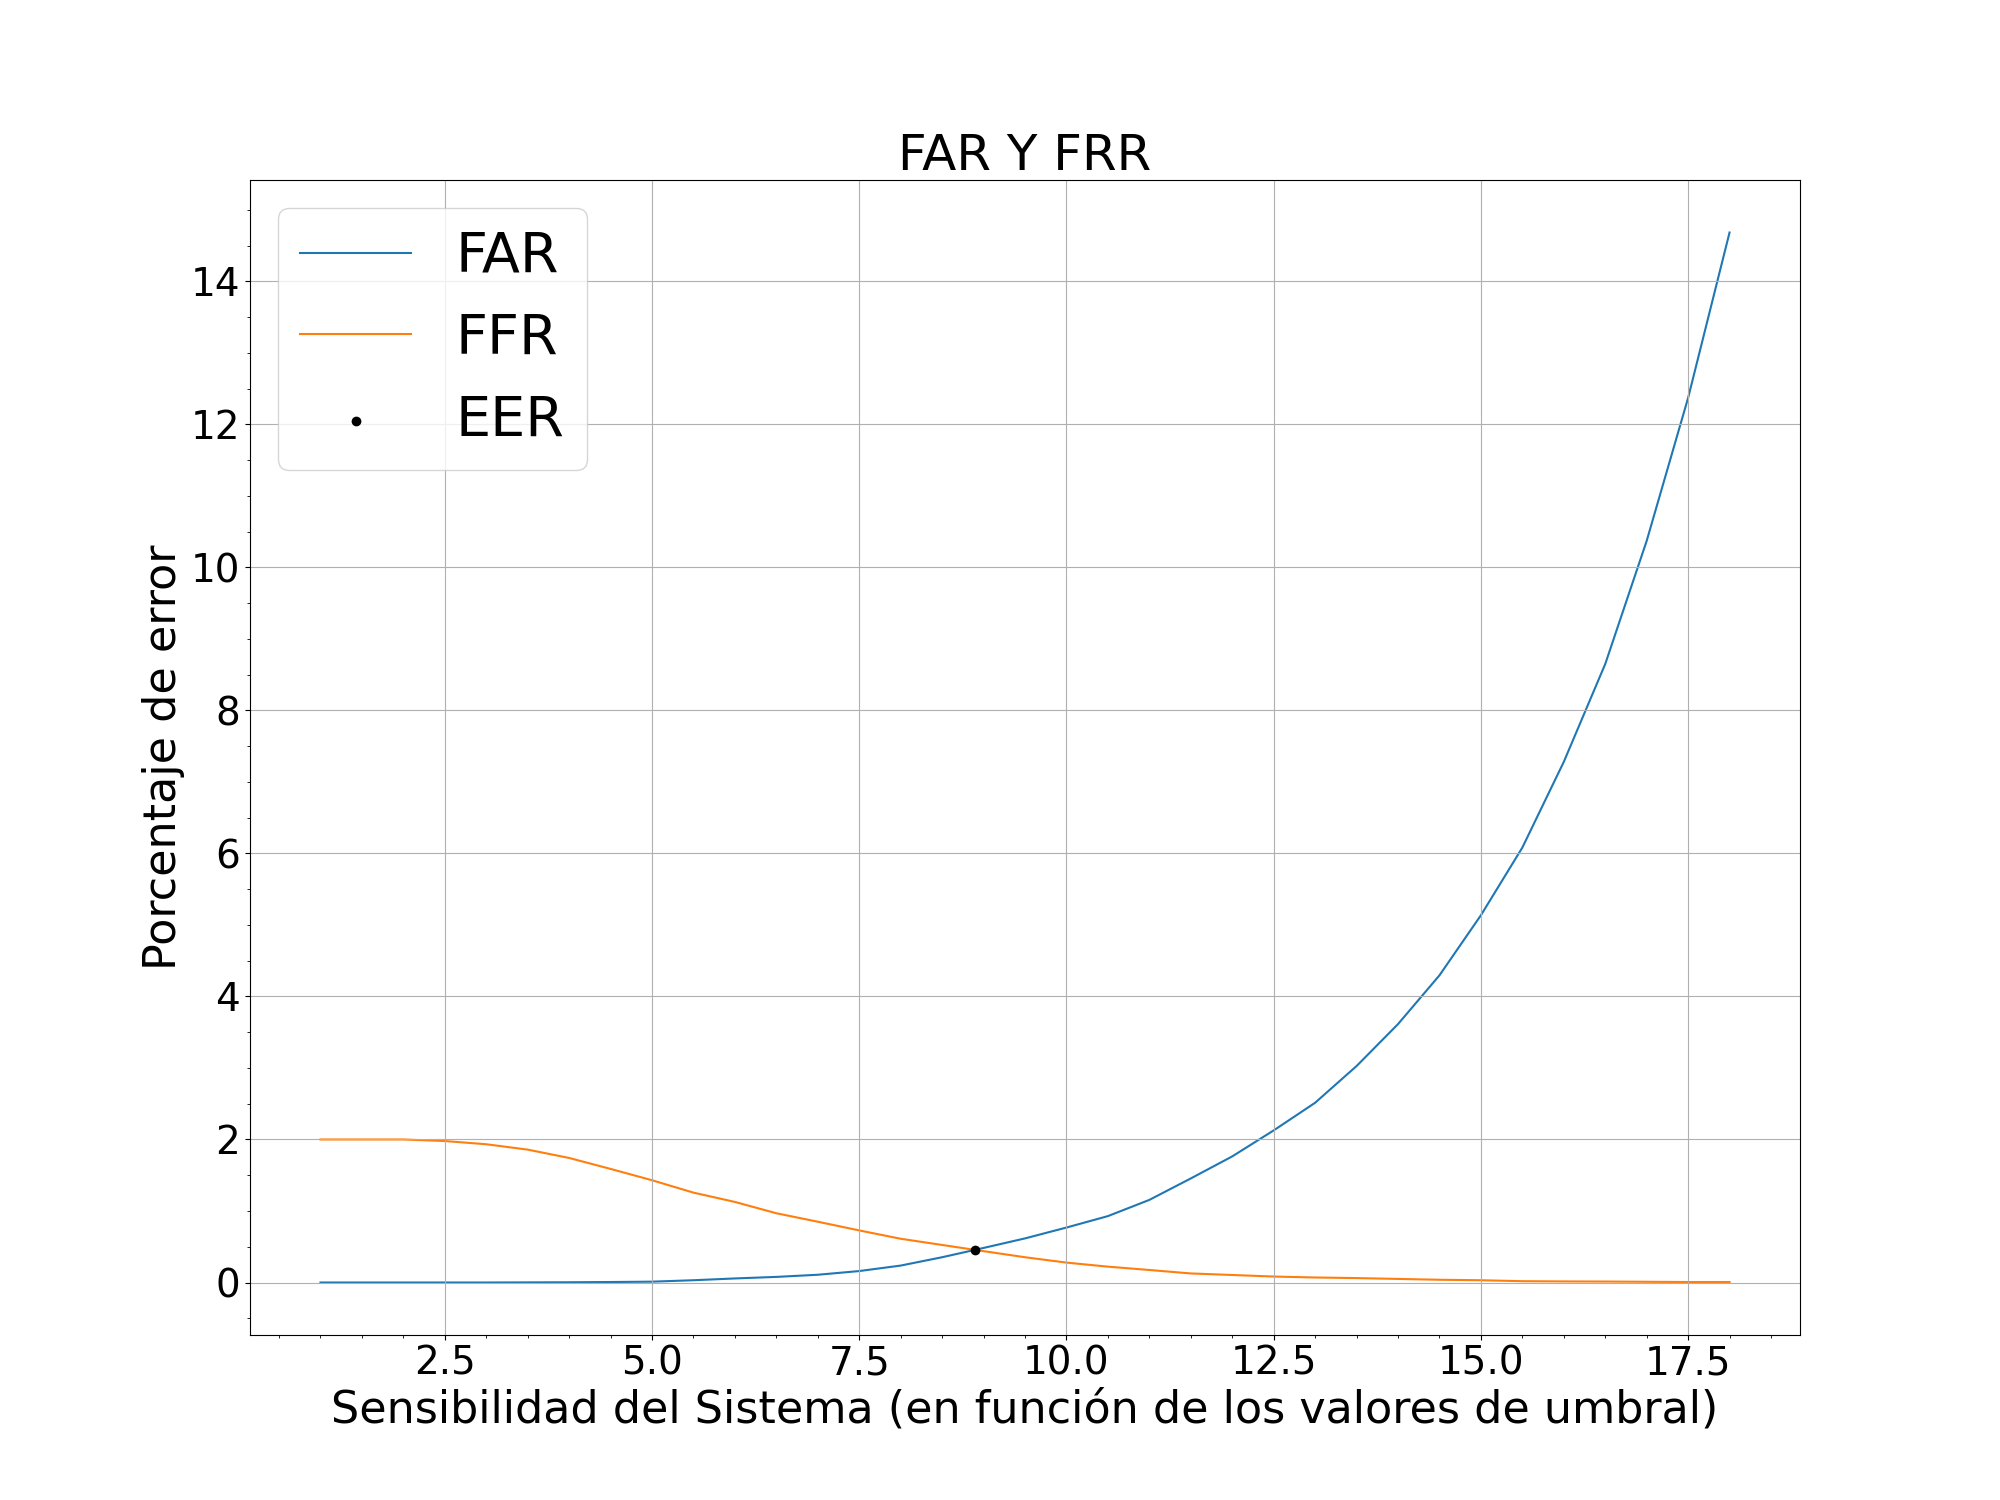
\includegraphics[width=0.85\textwidth]{/eer_24_2}
	\caption{Curvas FAR y FRR. El EER es el punto de intersecci�n entre ambas curvas.}
	\label{eer}
\end{figure}

El con el que se ha obtenido mejor EER  ha sido el 2, con un error de tan solo: \break \textbf{$EER_{2}$ = 0,46$\%$}. La Figura \ref{eer} muestra su EER obtenido haciendo uso de todas las muestras disponibles en el set de consulta.

Si comparamos el EER obtenido para los 3 modelos (Figura \ref{eer_compa}), nos encontramos con un peor valor para el primero ($EER_{1} = 0,81\%$). A�n as�, este valor de error sigue siendo significativamente bueno y, m�s a�n, si tenemos en cuenta que estamos utilizando una red que no ha sido entrenada con ninguna toma registrada despu�s de hacer ejercicio, para verificar la identidad de usuarios despu�s de haberlo realizado. 
Si nos fijamos en los resultados obtenidos para el 2� y el $3^{er}$ modelo, observamos que son pr�cticamente iguales ($EER_{3} = 0.49\%$), por lo que a primera vista parece que aumentar el porcentaje de sujetos con los que se ha realizado la fase de entrenamiento no ha supuesto una mejora.

\begin{figure}[H]
	\centering
	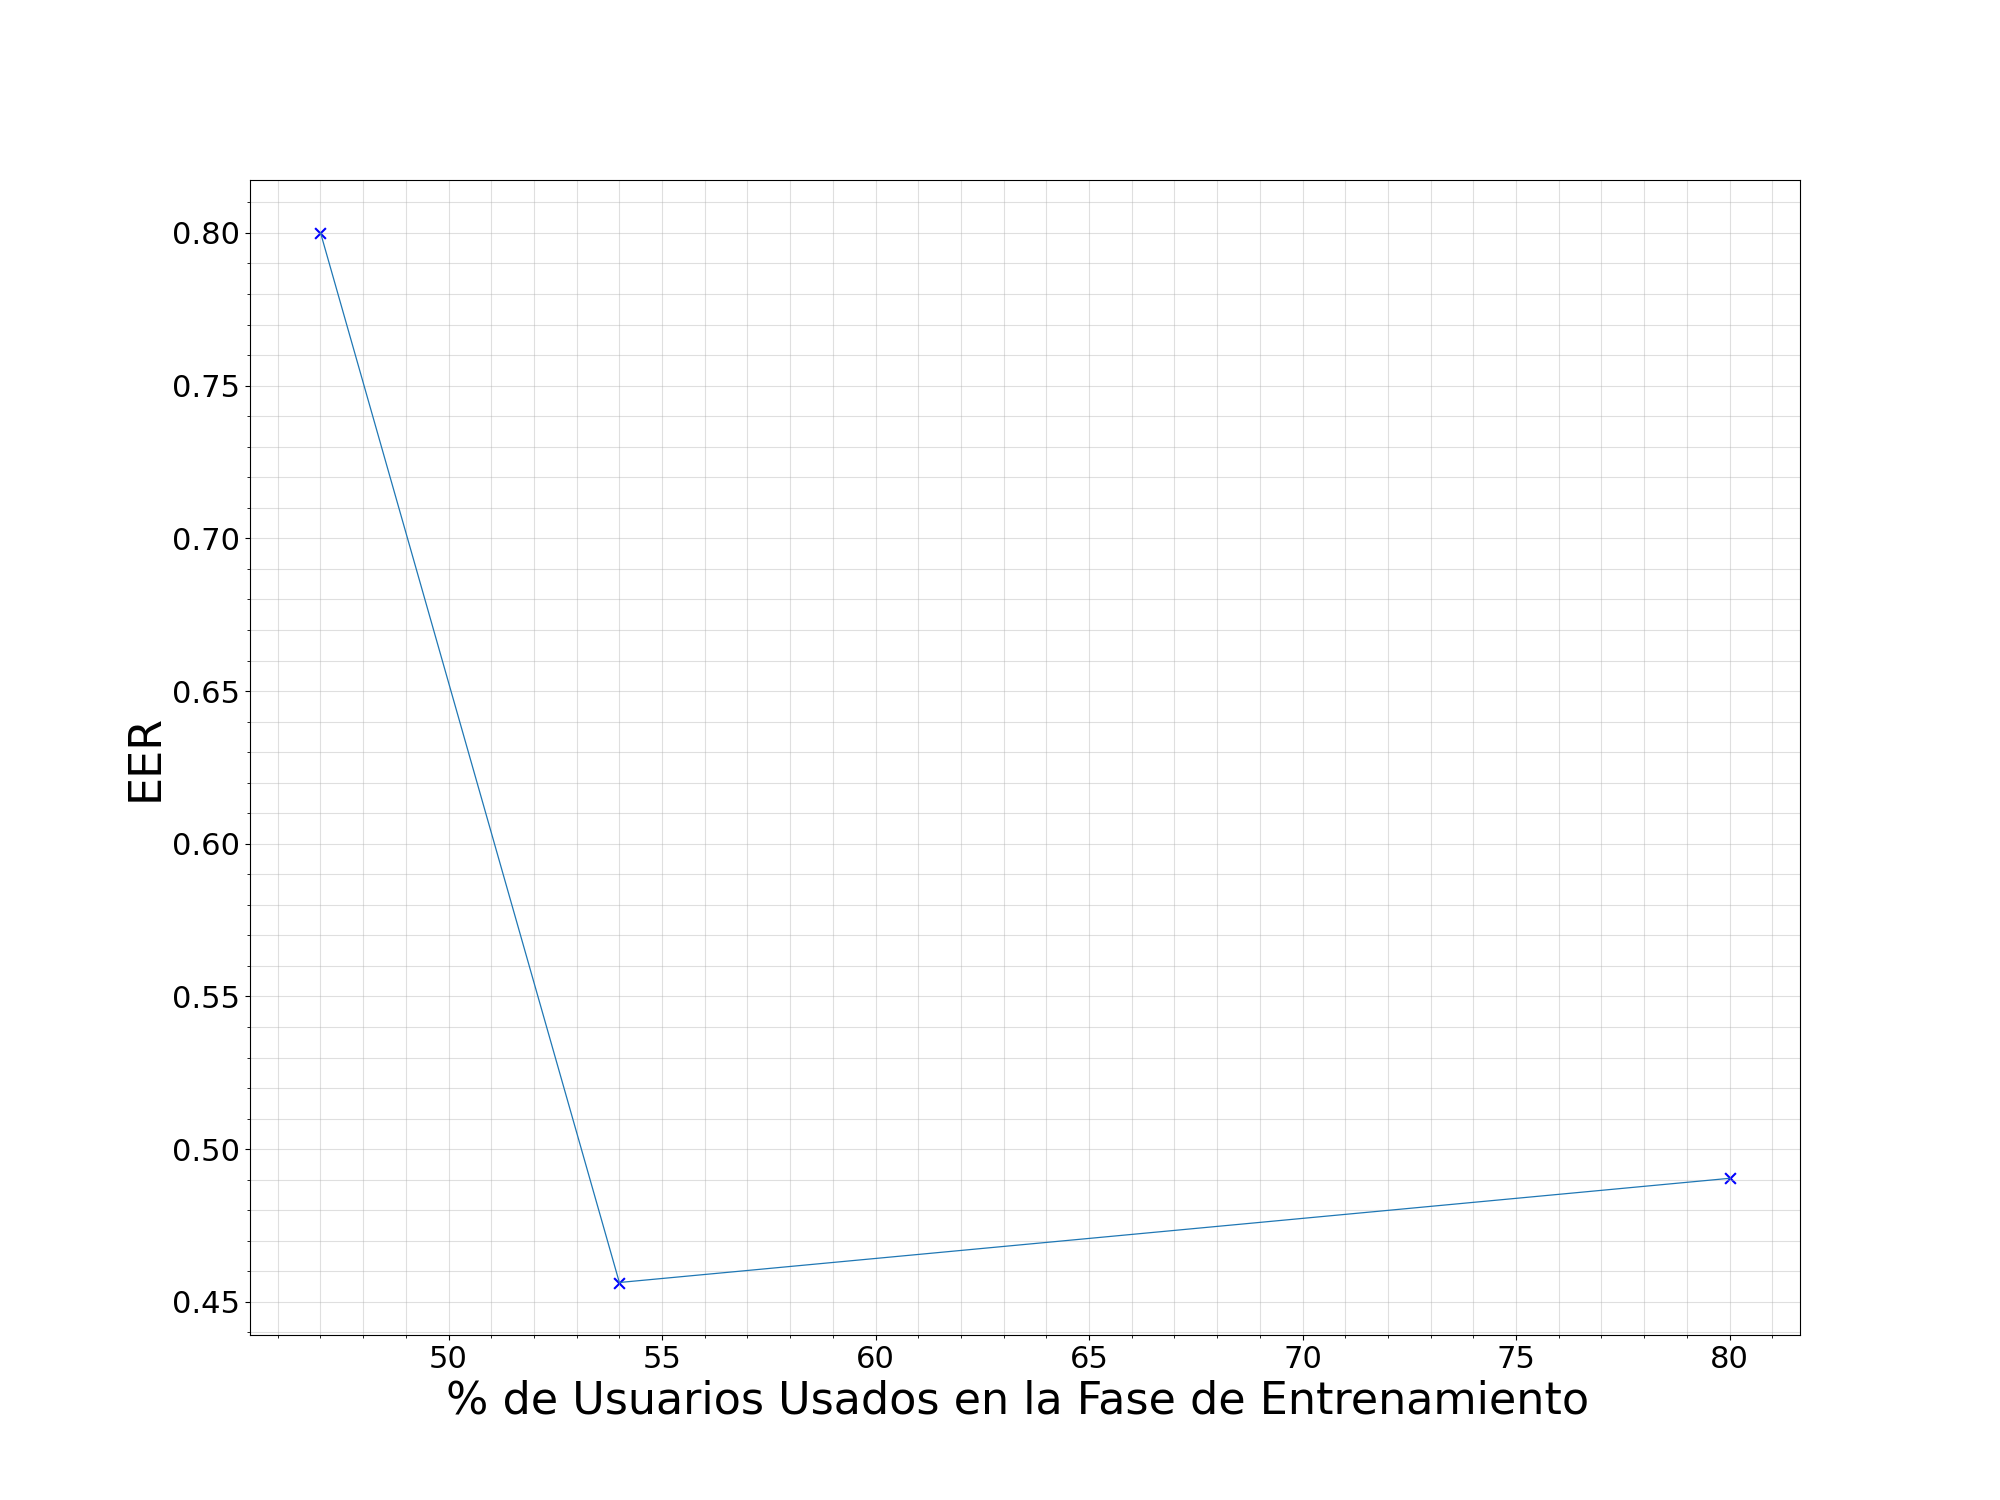
\includegraphics[width=0.85\textwidth]{/eer_compa}
	\caption{Comparaci�n del EER obtenido en funci�n del porcentaje de usuarios utilizado para el entrenamiento de la red.}
	\label{eer_compa}
\end{figure}

Para analizar m�s detalladamente el comportamiento del EER, se ha analizado su variabilidad en funci�n de las muestras de cada usuario
%del n�mero de muestras de cada usuario
que se utilizan para realizar las consultas. Para ello, se han ejecutado varias veces consultas con \textit{m} muestras por usuario. Estas \textit{m} muestras de cada usuario se seleccionan aleatoriamente de entre todas las disponibles cada vez que se realiza una ejecuci�n con $q = n \times (m \times n)$ consultas. 

En la Figura \ref{var} podemos ver la variaci�n m�xima del EER en funci�n del n�mero de muestras por usuario para cada modelo. Esta Figura muestra una clara tendencia en la que la variaci�n m�xima del EER disminuye a medida que aumenta el n�mero de muestras utilizado, en todos los modelos. Por tanto, el rendimiento del sistema depende en cierta medida de las muestras con las que se han realizado las consultas, y cuantas m�s consultas se realizan m�s fiable es el resultado obtenido. 

Adem�s, es muy significativa la diferencia de magnitud entre el Modelo 3 y los dem�s, con una variaci�n de m�s del doble en algunos de los casos. Este dato evidencia que el sistema es m�s fiable cuantas m�s consultas se realizan, pues en el Modelo 3 hay menos de la mitad de usuarios registrados y por tanto el n�mero de consultas que se pueden realizar con \textit{m} muestras es mucho menor. As�, cabr�a pensar que, si se pudiera hacer un mayor n�mero de consultas para evaluar este modelo s� obtendr�amos una mejora del rendimiento en funci�n del n�mero de usuarios utilizados para el entrenamiento, como se obtiene en \cite{autentiguia}.


\begin{figure}[H]
	\centering
	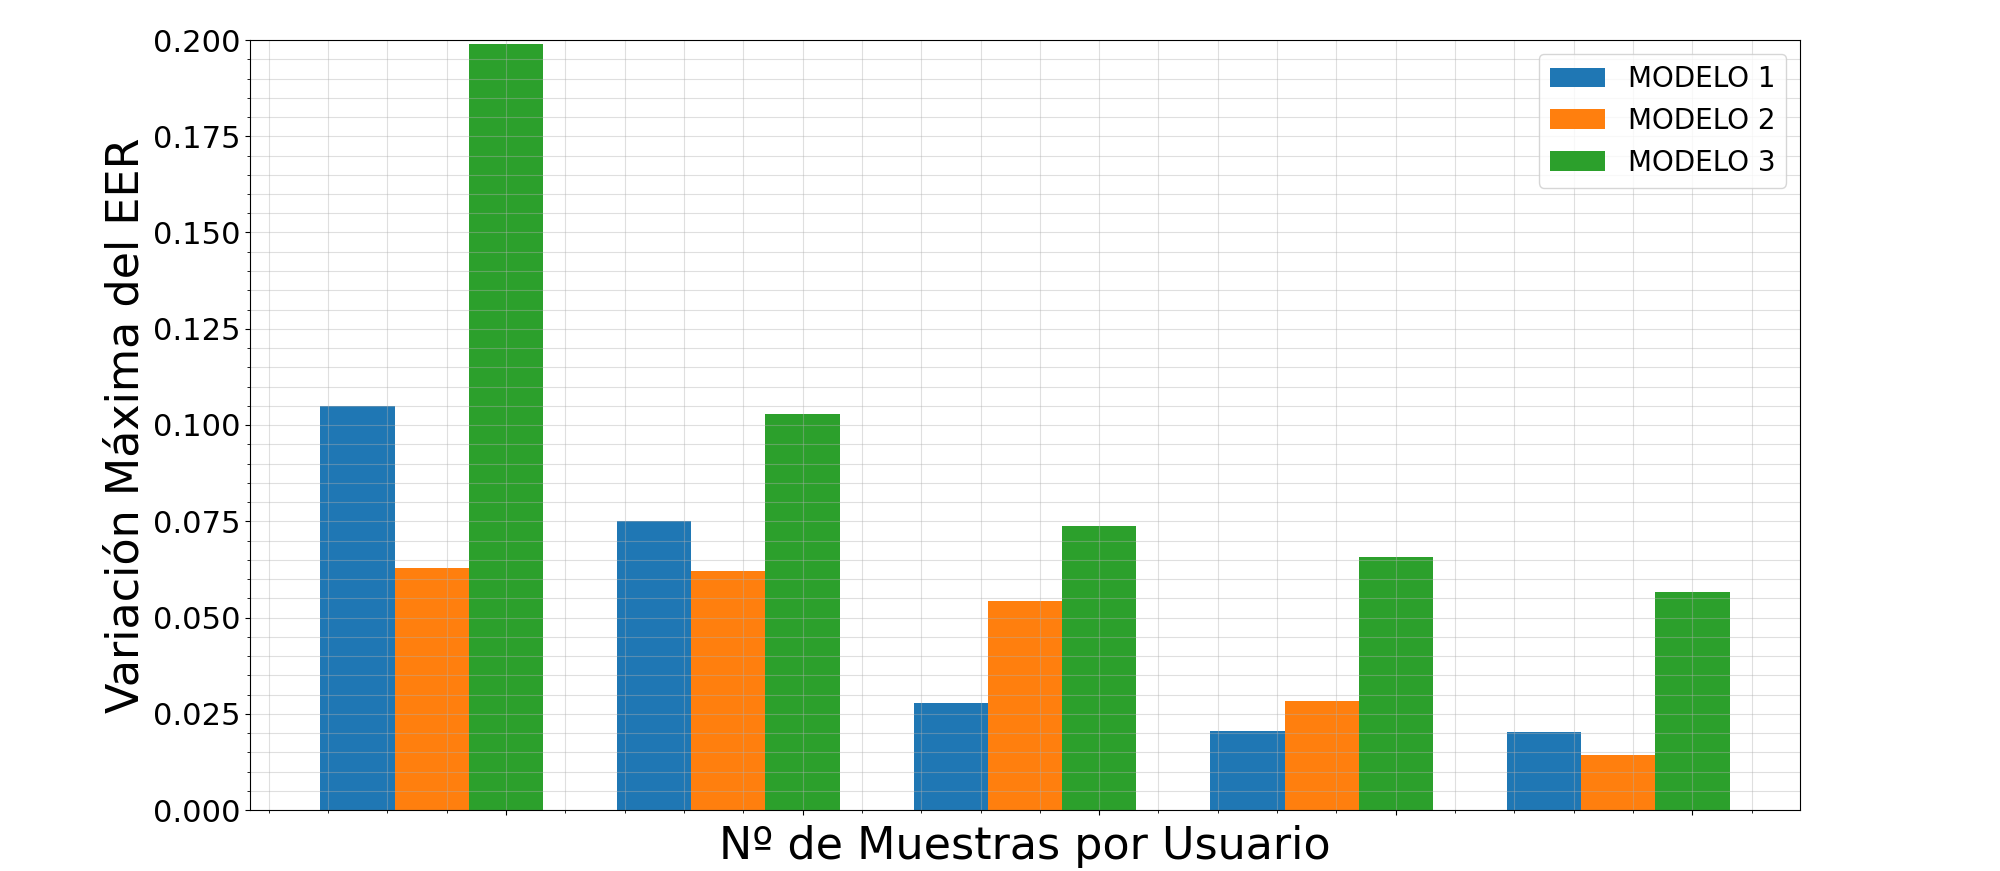
\includegraphics[width=0.9\textwidth]{/var_}
	\caption{Variabilidad del resultado de error obtenido en funci�n de las muestras utilizadas.}
	\label{var}
\end{figure}

En la siguiente Figura (\ref{var_eer}) podemos ver un ejemplo de los EER obtenidos utilizando \textit{m} muestras aleatorias de cada usuario. Teniendo en cuenta la variaci�n de este error que acabamos de comentar, podemos ver c�mo aunque se haya obtenido un mejor error para un \textit{m} menor, este resultado depende de las muestras que se hayan utilizado para ese caso concreto, mientras que si aumenta el n�mero de muestras utilizado el resultado es m�s fiable. 
\newline
\begin{figure}[H]
	\centering
	\subfigure[MODELO 1]{
		\label{fig:err1}
		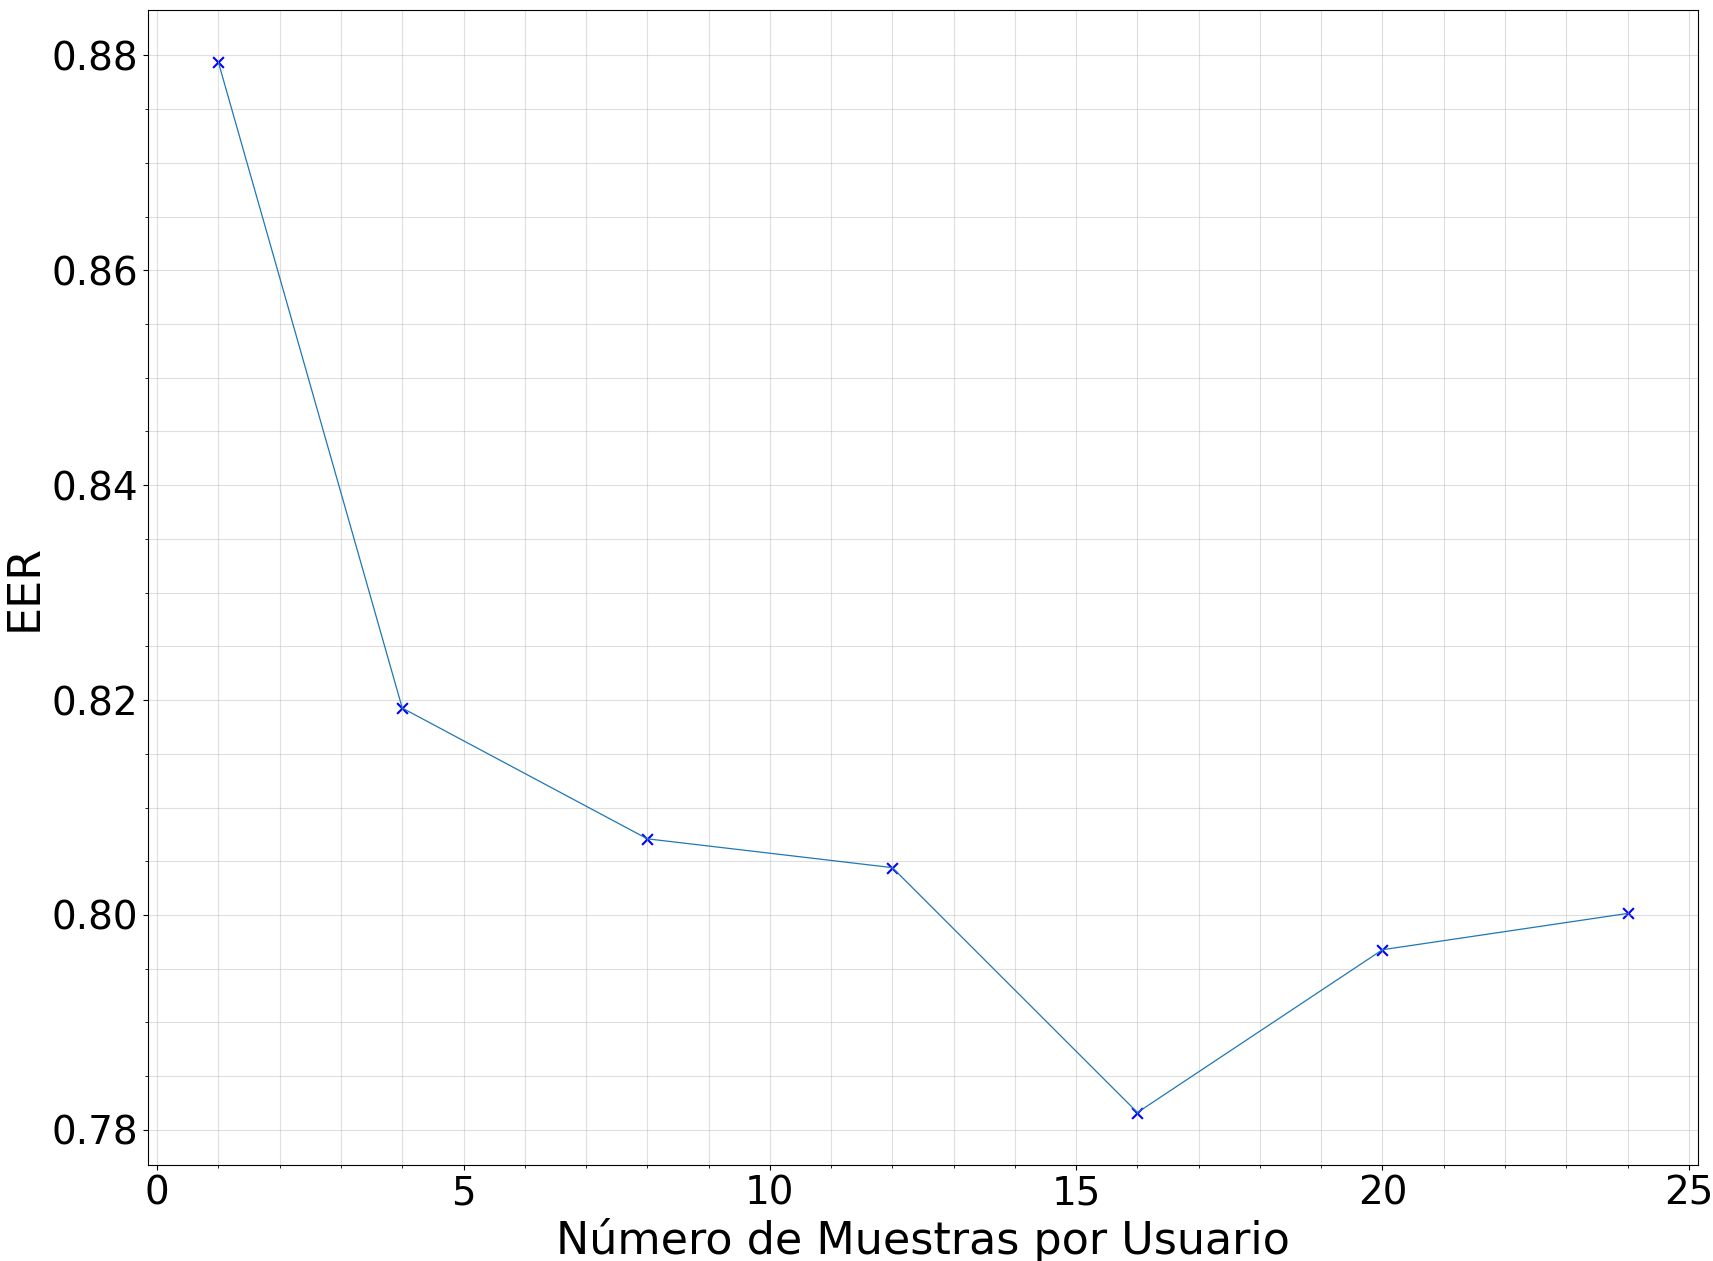
\includegraphics[width=0.3\textwidth]{/eer_1_}}
	\subfigure[MODELO 2]{
		\label{fig:eer2}
		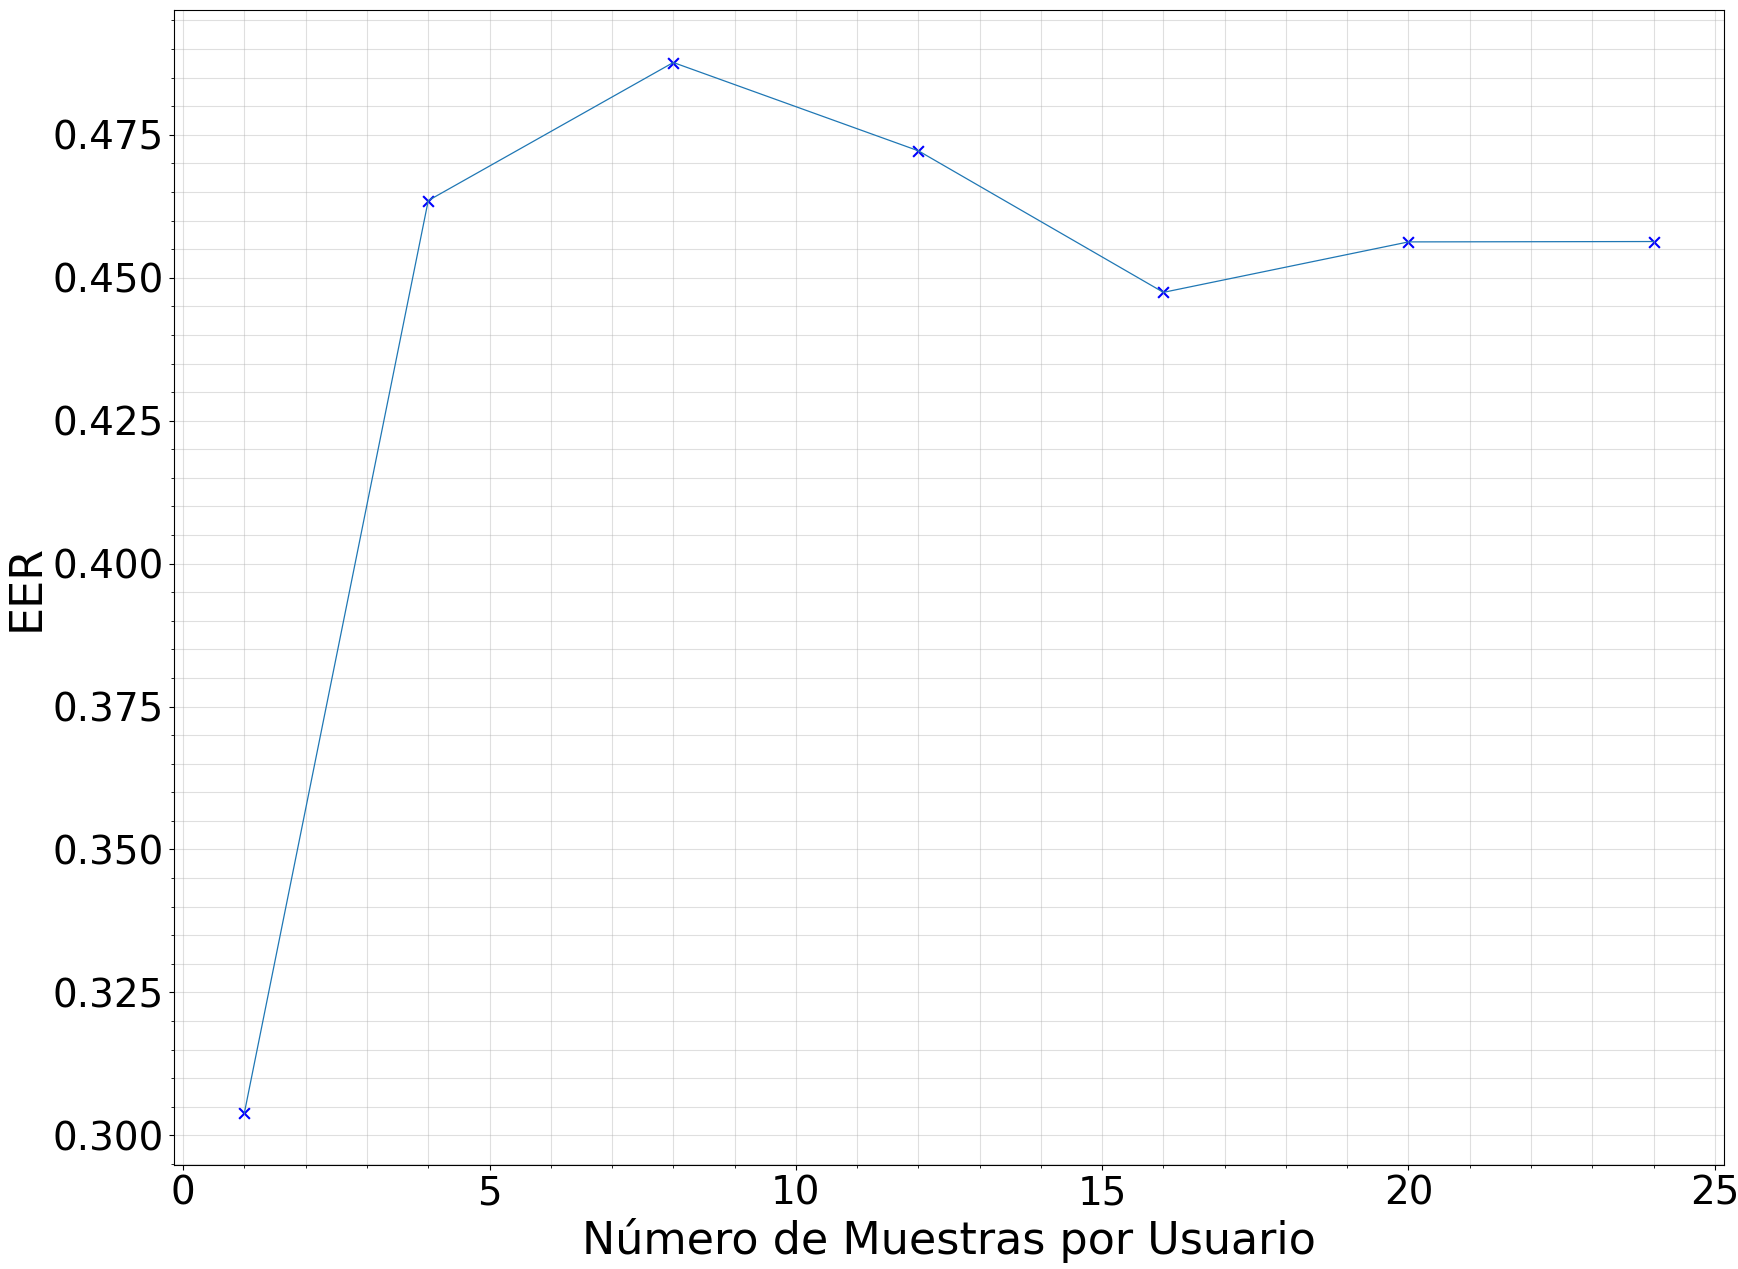
\includegraphics[width=0.3\textwidth]{/eer_2_}}
	\subfigure[MODELO 3]{
		\label{fig:eer3}
		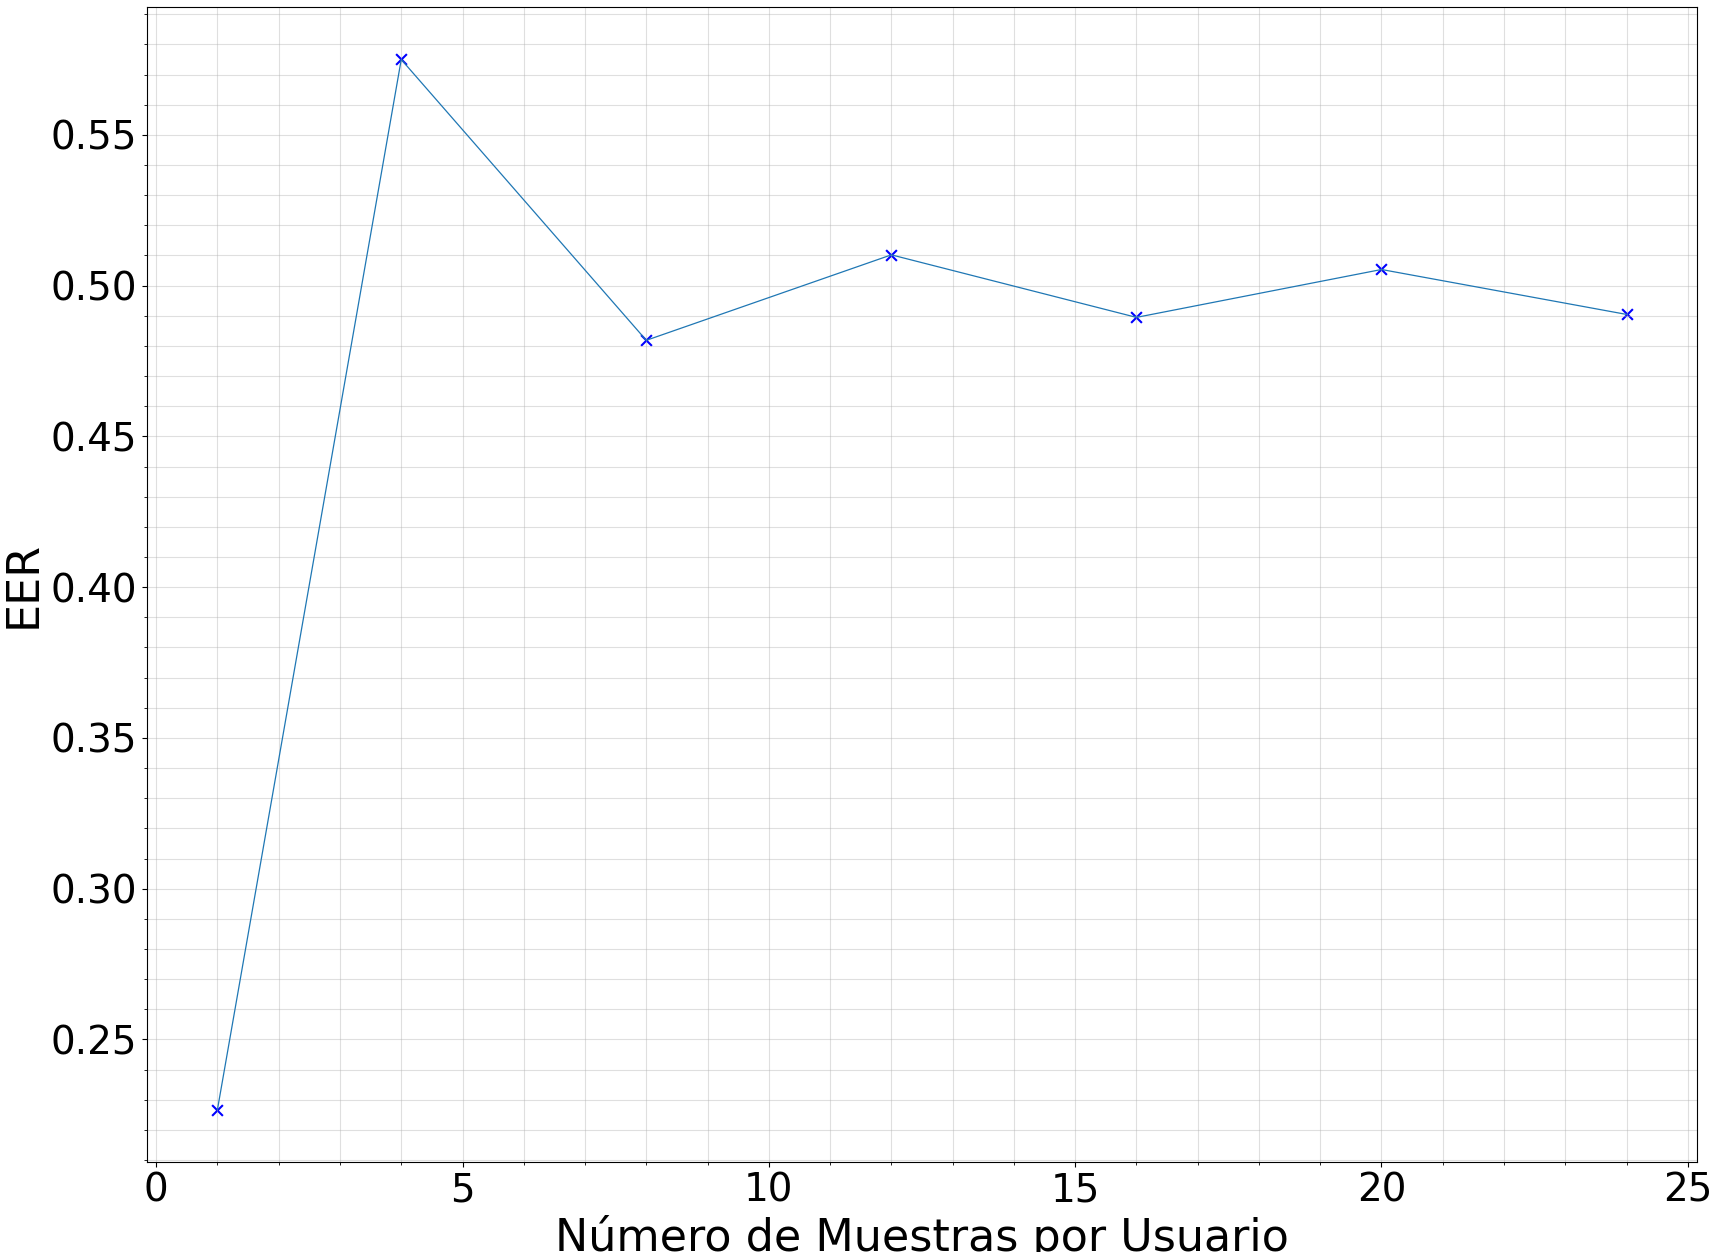
\includegraphics[width=0.3\textwidth]{/eer_3_}}
	\caption{Variaci�n del EER en funci�n del n�mero de muestras.}
	\label{var_eer}
\end{figure} 


%Adem�s, la siguiente FIG muestra c�mo var�a el EER en funci�n del n�mero de consultas que se hacen para cada modelo, o dicho de otra manera, el n�mero de muestras $m_i$ de cada usuario con las que se realizan las consultas. Si se han realizado $q$ consultas, quiere decir que el n�mero de muestras que se ha utilizado de \underline{cada} usuario es $ m_i = \dfrac{q}{n \times n}$. Estas $m_i$ muestras de cada usuario se cogen aleatoriamente de las $\dfrac{m}{n}$ muestras posibles.









Por �ltimo, se ha comparado el rendimiento de los tres modelos mediante la curva ROC (\textit{Receiver Operating Characteristic curve}). En ella se representa el FAR frente a TAR (\textit{True Acceptance Rate}).

\begin{center}
	$TAR =  1 - FRR $
\end{center}

Esta curva es independiente del umbral y permite la comparaci�n del rendimiento de diferentes sistemas bajo unas condiciones similares \cite{iso}.

\begin{figure}[H]
	\centering
	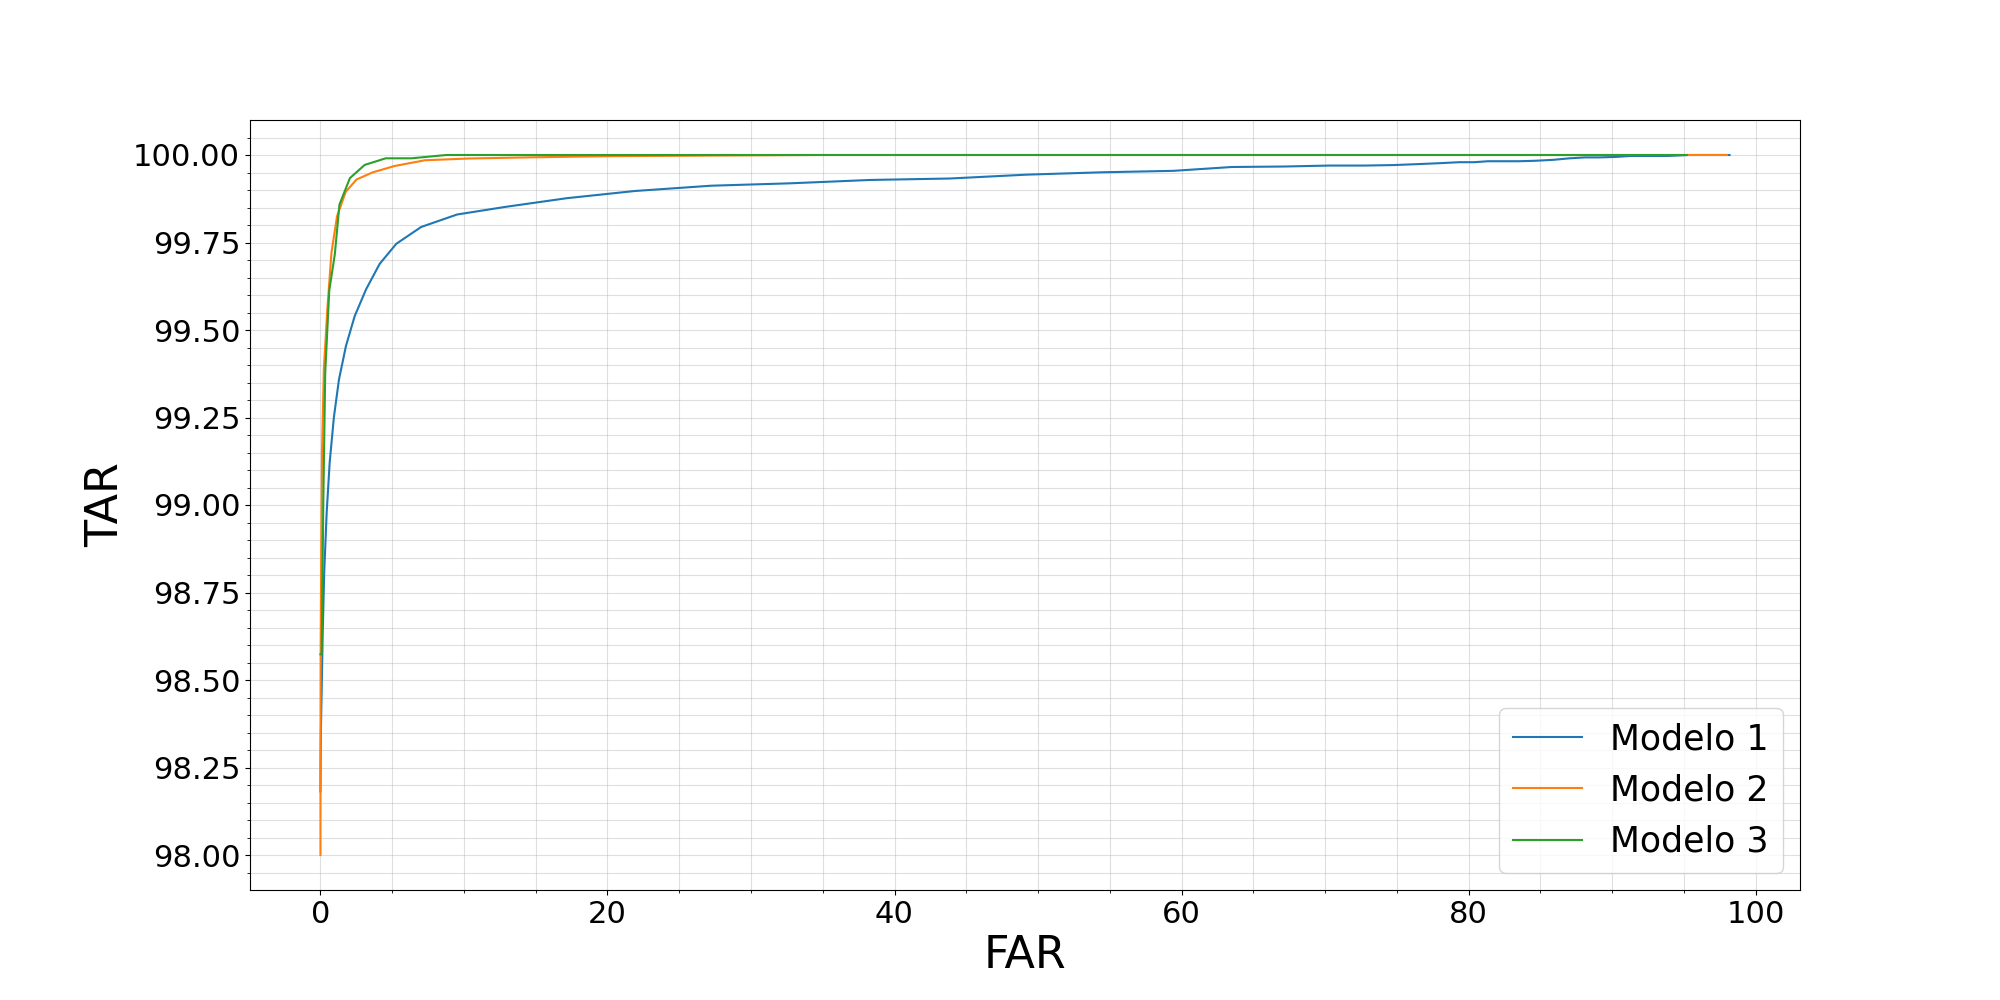
\includegraphics[width=1\textwidth]{/roc_definitiva}
	\caption{Comparaci�n del rendimiento de los tres modelos con la curva ROC.}
	\label{roc}
\end{figure}

Como se puede apreciar en la Figura \ref{roc}, el sistema con un peor rendimiento es el Modelo 1, en el que la curva no se acerca tanto a la esquina izquierda. A�n as�, la curva obtenida para los tres modelos permite confirmar que puede realizarse la verificaci�n de usuarios obteniendo buenos resultados con cualquiera de ellos. 
%%%%%%%%%%%%%%%%%%%%%%%%%%%%%%%%%%%%%%%%%%%%%%%%%%%%%%%%%%%%%%%%%%%%%%%%%%%%%%%!
%
% -- Resultados.tex --
%    Resultados y conclusiones
%
%%%%%%%%%%%%%%%%%%%%%%%%%%%%%%%%%%%%%%%%%%%%%%%%%%%%%%%%%%%%%%%%%%%%%%%%%%%%%%%!
%!TEX root = ../../Principal/TFG.tex
\chapter{Conclusiones}
\label{chap:conclusiones}
\pagestyle{fancy}
\thispagestyle{empty}
%
\graphicspath{{../Conclusiones/Imagenes/}}
\DeclareGraphicsExtensions{.pdf,.jpg,.png}
%
% Empieza a escribir aqu�
\section{Conclusiones}

Con este proyecto, se ha querido probar la fiabilidad que ofrece la actividad el�ctrica del coraz�n registrada con el ECG como una caracter�stica biom�trica, que permita tanto la identificaci�n de usuarios, como su autenticaci�n. Para ello, se ha dise�ado un sistema basado en redes neuronales convolucionales (CNN), con las que se ha realizado una extracci�n de caracter�sticas, indicando qui�n es el usuario registrado m�s cercano, en el caso de la identificaci�n, y obteniendo patrones biom�tricos, en el caso de la verificaci�n de identidad. 

Adem�s, se ha evaluado el sistema implementado para ambas modalidades biom�tricas, haciendo uso de una base de datos especialmente dise�ada para el reconocimiento de usuarios a trav�s de su ECG. Esta base de datos incluye muestras de 105 usuarios registradas en dos sesiones diferentes para cada uno, separadas entre s� por un m�nimo de una semana. En estas sesiones, se han llevado a cabo diferentes experimentos para el registro de la se�al, incluyendo tomas en las que el usuario se encuentra sentado, de pie e, incluso, tomas realizadas despu�s de someter al usuario a un ejercicio f�sico, acelerando el ritmo card�aco hasta llegar a los 130 latidos por minuto. Con ello, hemos querido probar tanto la unicidad del ECG como caracter�stica biom�trica, como su estabilidad.

En primer lugar, estas se�ales han sido sometidas a una fase de preprocesamiento, que incluye el filtrado de la se�al, su segmentaci�n basada en la detecci�n de picos R, y la obtenci�n de un vector formado por 8 complejos QRS concatenados. Este vector se ha utilizado como entrada (\textit{input}) de una red neuronal, que ha permitido llevar a cabo el reconocimiento de usuarios. 

En el caso de la identificaci�n, se han realizado diferentes pruebas para un conjunto cerrado (\textit{closed set}) de los usuarios de la base de datos. Por un lado, se ha demostrado que la identificaci�n de 50 usuarios, cuyas tomas de ECG han sido registradas en dos sesiones diferentes, se puede conseguir con una exactitud del \textbf{97,58\%}. Adem�s, si se eval�a el rendimiento del sistema con 55 usuarios cuyas tomas, adem�s de haber sido registradas en dos sesiones diferentes, incluyen muestras en las que el usuario se encontraba tanto sentado como de pie, y tanto en reposo como despu�s de haber realizado deporte, la exactitud obtenida ha sido del \textbf{ 97,39\%}. Finalmente, la evaluaci�n del sistema utilizando los 105 usuarios juntos, ha permitido demostrar la unicidad del ECG como caracter�stica biom�trica, con un rendimiento del \textbf{95,59\%}. Esta disminuci�n de la exactitud obtenida al aumentar el n�mero de sujetos se ve condicionada, en parte, por una optimizaci�n de hiperpar�metros menos que se ha realizado de manera menos exhaustiva que en el caso de los otros dos modelos. 

En cuanto a la estabilidad del ECG para su uso en la identificaci�n de usuarios, s� podemos confirmar que el rendimiento del sistema es muy elevado cuando ha sido entrenado con registros de diferentes d�as y bajo diferentes condiciones. Sin embargo, no hemos podido probar que el ECG sea una caracter�stica estable, pues el rendimiento del sistema ha disminuido notablemente cuando el entrenamiento se ha realizado con tomas registradas un d�a diferente al d�a de registro de las tomas utilizadas para su evaluaci�n, siendo, adem�s, el n�mero de usuarios de la base de datos no excesivamente alto.

En el caso de la autenticaci�n, la evaluaci�n del sistema se ha realizado con usuarios diferentes a los utilizados para el entrenamiento de la red neuronal. De esta manera, ha sido posible verificar la identidad de 55 usuarios, cuyas muestras hab�an sido registradas incluyendo la condici�n del ejercicio, con un sistema entrenado sin este tipo de muestras, con un EER del \textbf{0,81\%}. Si adem�s, el sistema s� es entrenado con muestras bajo esta condici�n, se consigue una mejora del rendimiento del sistema, obteniendo un EER de tan solo el \textbf{0,45\%}.

Estos resultados obtenidos para ambas modalidades, nos permiten confirmar que el ECG se puede utilizar para el reconocimiento biom�trico con un rendimiento muy elevado, demostrando que esta novedosa t�cnica es potencialmente prometedora.

La comparaci�n de los resultados obtenidos en este proyecto con otros estudios, basados tambi�n en redes neuronales, se puede observar en la siguiente Tabla \ref{final}.


%\begin{table}[H]
%	\centering
%	\begin{tabularx}{0.9\textwidth}{ 
%			%c c c c c c }
%			>{\raggedright\arraybackslash}X
%			>{\centering\arraybackslash}X
%			>{\centering\arraybackslash}X
%			>{\centering\arraybackslash}X
%			>{\centering\arraybackslash}X
%			>{\raggedleft\arraybackslash}X}
%		
%		Autor & Usuarios & Preprocesado & M�todo & Tasa de Identificaci�n & EER de autenticaci�n \\
%		\hline
%		Labati \textit{et al.} \cite{deepecg} & 52 & Parcialmente-local & CNN & 100\% & - \\
%		\hline
%		Zhang \textit{et al.} \cite{Zhang2017}& 18 a 47 & Sin preprocesar & CNN & 93,5\% & - \\
%		\hline
%		Zhang \textit{et al.} \cite{Zhang2018}& 18 a 47 & Parcialmente-local & CNN & 95\% & - \\
%		\hline
%		Pinto \textit{et al.} \cite{Pinto2019}& 1019 & Sin preprocesar &CNN  & - & 7,86\% \\
%		\hline
%		Pinto \textit{et al.} \cite{deep}& 1019 & Sin preprocesar & CNN & 96,1\% & - \\
%		\hline
%		Salloum {et al.} \cite{autentiguia}& 47 &  Parcialmente-local & RNN & 100\% & 0\% \\
%		\hline
%		Estudio propuesto & 105 &  Parcialmente-local & CNN & 95,59\% & 0,45\% \\
%		\hline
%		
%	\end{tabularx}
%\caption{Comparativa de estudios existentes basados en redes neuronales para la identificaci�n y autenticaci�n biom�trica a trav�s del ECG.}
%\label{final}
%\end{table}

\begin{table}[H]
	\centering
	%\begin{tabularx}{1\textwidth}{ 
	%		%c c c c c c }
	%		>{\raggedright\arraybackslash}X
	%		>{\centering\arraybackslash}X
	%		>{\centering\arraybackslash}X
	%		>{\centering\arraybackslash}X
	%		>{\centering\arraybackslash}X
	%		>{\raggedleft\arraybackslash}X}
	\resizebox{\textwidth}{!}{%
		\begin{tabular}{c c c c c c }
			\hline
			Autor & Usuarios & Preprocesado & M�todo & Tasa de Identificaci�n & EER de autenticaci�n \\
			\hline
			Labati \textit{et al.} \cite{deepecg} & 52 & Parcialmente-local & CNN & 100\% & 1,05 \\
			\hline
			Zhang \textit{et al.} \cite{Zhang2017}& 18 a 47 & Sin preprocesar & CNN & 93,5\% & - \\
			\hline
			Zhang \textit{et al.} \cite{Zhang2018}& 18 a 47 & Parcialmente-local & CNN & 95\% & - \\
			\hline
			Pinto \textit{et al.} \cite{Pinto2019}& 1019 & Sin preprocesar &CNN  & - & 7,86\% \\
			\hline
			Pinto \textit{et al.} \cite{deep}& 1019 & Sin preprocesar & CNN & 96,1\% & - \\
			\hline
			Salloum {et al.} \cite{autentiguia}& 47 &  Parcialmente-local & RNN & 100\% & 0\% \\
			\hline
			Sistema propuesto & 105 &  Parcialmente-local & CNN & 95,59\% & 0,45\% \\
			\hline
			
	\end{tabular}}
	\caption{Comparativa de estudios existentes basados en redes neuronales para la identificaci�n y autenticaci�n biom�trica a trav�s del ECG.}
	\label{final}
\end{table}
 

Por �ltimo, cabe destacar el bajo coste computacional que requiere tanto la fase de identificaci�n como la fase de consulta de la verificaci�n de la identidad. Para la implementaci�n de este estudio, se ha utilizado un ordenador port�til con un procesador Intel(R) Core(TM) i7-8550U CPU de 1,8GHz, con una RAM de 12 GB. El tiempo de identificaci�n de cada muestra ha sido de 0,478 ms y el tiempo para la comparaci�n de patrones en autenticaci�n ha sido de 0,609 ms  para cada consulta. Estos valores tan bajos, permiten que estos sistemas se puedan llegar a emplear en escenarios reales para el reconocimiento biom�trico.


\section{Lineas futuras}


En esta secci�n, presentamos posibles l�neas futuras de trabajo que podemos introducir gracias a este proyecto:

\begin{itemize}

	\item Mejorar el rendimiento del sistema de identificaci�n cuando aumenta el n�mero de usuarios registrados, llevando a cabo una b�squeda m�s exhaustiva de hiperpar�metros del modelo.
	\item Dise�ar y desarrollar un sistema de identificaci�n de usuarios de un conjunto abierto (\textit{open set}). Para ello, bastar�a con determinar un umbral en el sistema implementado en este proyecto, que permitiera clasificar al usuario como no registrado, cuando la probabilidad de pertenecer a una de las clases registradas no sea en ning�n caso superior a dicho umbral.
	\item Implementar un sistema basado en redes neuronales convolucionales con una fase de preprocesado menos compleja, que permita el reconocimiento de usuarios a partir de fragmentos de las se�ales de ECG, sin la necesidad de ser segmentadas en base a la detecci�n de picos R. 
	\item Demostrar la estabilidad del ECG como caracter�stica biom�trica para ambas modalidades, consiguiendo una mejora del rendimiento del sistema cuando se trabaja con muestras registradas en diferentes sesiones y bajo diferentes condiciones. Para ello, se podr�a implementar una base de datos multisesi�n propia, que incluya tomas de diferentes d�as y horas, adem�s de diferentes situaciones que generen alteraciones del ritmo card�aco del usuario (actividades deportivas, pruebas de estr�s, etc).
\end{itemize}
%Identificaci�n open set
%Identificaci�n muestras diferentes d�as 
%
%Autenticaci�n muestras tambi�n diferentes d�as
%
%Reducir la complejidad de la fase de preprocesado, redes directamente con fragmento de se�al ``raw''




%-----------------------------------------------------------------------------%

%-----------------------------------------------------------------------------%
\null\pagestyle{fancy}\newpage\null\pagestyle{empty}\clearpage
\renewcommand{\chapformat}[1]{%
	\parbox[b]{0.75\textwidth}{\filleft\sf\bfseries #1}%
	\quad\rule[-12pt]{2pt}{100pt}\quad\hspace{2mm}{\hspace{2mm}}}
\pagenumbering{roman}
\appendix
%\backmatter
%!TEX root = ../../Principal/TFG.tex
\chapter{Anexo I: Calidad de las clasificaciones obtenidas en identificaci�n}
\label{appe:A}
\pagestyle{fancy}
\thispagestyle{empty}
%
\graphicspath{{../ApendiceA/Imagenes/}}
\DeclareGraphicsExtensions{.pdf,.png,.jpg}

% Empieza a escribir aqu�
\section{Base de datos 1}

\begin{table}[h]{
	\centering
	\includegraphics[width=1.1\textwidth]{/clasif1_}}
\caption{Calidad de las clasificaciones obtenidas para cada usuario de la primera base de datos.}
\label{clasif1}
\end{table}
\newpage

\section{Base de datos 2}


\begin{table}[h]{
		\centering
		\includegraphics[width=1.1\textwidth]{/clasif2}}
	\caption{Calidad de las clasificaciones obtenidas para cada usuario de la segunda base de datos.}
	\label{clasif2}
\end{table}	

\newpage


\section{Base de datos completa}\label{appe:A3}

% \vfill
% \begin{center}


\begin{table}[h]{
%		\centering
		
		\includegraphics[width=1\textwidth]{/medias}}
	\caption{Calidad de las clasificaciones obtenidas para la base de datos completa.}
	\label{report_}
\end{table}	


%\vfill

\begin{figure}[h]{
		%\centering
		\includegraphics[width=1\textwidth]{/clasif_}}
	\caption{Calidad de las clasificaciones obtenidas para cada usuario de la base de datos completa.}
	\label{clasif_todo}
\end{figure}

%\end{center}
%\vfill

%!TEX root = ../../Principal/TFG.tex
\chapter{ Anexo II: Visualizaci�n de los vectores de caracter�sticas con la herramienta PCA}
\label{appe:C}
\pagestyle{fancy}
\thispagestyle{empty}
%
\graphicspath{{../ApendiceC/Imagenes/}}
\DeclareGraphicsExtensions{.pdf,.png,.jpg}
%


Si visualizamos los vectores de caracter�sticas obtenidos durante la fase de reclutamiento utilizando la herramienta PCA (an�lisis de componentes principales, ACP, en castellano), las agrupaciones por usuario, que ve�amos bien definidas en el espacio con la herramienta TSNE, dejan de ser tan evidentes, y solo un reducido n�mero de usuarios parece estar distanciado del resto. 
\newline

\begin{figure}[h!]
	\centering
	\subfigure[MODELO 1]{
		\label{fig:pca1}
		\includegraphics[width=0.32\textwidth]{/pca1}}
	\subfigure[MODELO 2]{
		\label{fig:pca2}
		\includegraphics[width=0.32\textwidth]{/pca2}}
	\subfigure[MODELO 3]{
		\label{fig:pca3}
		\includegraphics[width=0.32\textwidth]{/pca3}}
	\caption{Comparativa de la distribuci�n de los vectores de caracter�sticas obtenidos durante la fase de reclutamiento para cada modelo, empleando la herramienta de visualizaci�n PCA para reducir a tres dimensiones el espacio.}
	\label{pca}
\end{figure}
%!TEX root = ../../Principal/TFG.tex
\chapter{Anexo III: Aspectos �ticos, econ�micos, sociales y ambientales}
\label{appe:B}
\pagestyle{fancy}
\thispagestyle{empty}
%
\graphicspath{{../ApendiceB/Imagenes/}}
\DeclareGraphicsExtensions{.pdf,.png,.jpg}
%

% Empieza a escribir aqu�

En este proyecto se ha implementado un sistema biom�trico a trav�s del ECG. Los sistemas biom�tricos se aplican mayoritariamente en el �mbito de la seguridad y, actualmente, son utilizados en numerosas ocasiones para el control de acceso, al tratarse de caracter�sticas propias de cada persona, intransferibles y dif�ciles de falsificar. Por ejemplo, esta tecnolog�a tiene un gran impacto en el control fronterizo, donde nuestra identidad es verificada, detectando posibles falsificaciones de documentos y contrastando nuestra informaci�n con las bases de datos disponibles en el control en relaci�n a posibles antecedentes. En este sentido, ya se est�n
implantando proyectos piloto en Espa�a donde el paso fronterizo se encuentra automatizado y se utilizan como rasgos para la verificaci�n la cara y la huella dactilar (Automatic Border Crossing (ABC)) \cite{econo}; agilizando de esta manera los tiempos en los controles y aumentando su seguridad.

Otro �mbito en el que esta tecnolog�a presenta un gran impacto es la banca, debido a la gran necesidad de aumentar la seguridad de sus operaciones, previniendo y evitando los fraudes en este sector. Hoy en d�a, la mayor�a de las operaciones bancarias dependen de la autenticaci�n de los usuarios basada en el uso de una gran cantidad de claves (contrase�as, firmas digitales, tockens...). Sin embargo, estos sistemas de autenticaci�n son altamente vulnerable en comparaci�n con los sistemas de autenticaci�n biom�trica. Por ejemplo, las transacciones a trav�s de tel�fonos m�viles podr�an beneficiarse de estos novedosos sistemas biom�tricos, verificando la identidad de los usuarios en todo momento a trav�s de sus rasgos, dif�cilmente suplantables. La biometr�a junto a la tecnolog�a NFC (Near Field Communication), presente en la gran parte de tel�fonos m�viles, es una de las aplicaciones con m�s futuro para garantizar la seguridad en las transacciones. 

Si adem�s tenemos en cuenta este nuevo enfoque del reconocimiento biom�trico a trav�s del ECG, nos encontramos con una mejora en el campo de la seguridad y el reconocimiento de usuarios, en comparaci�n con la gran mayor�a de modalidades existentes: la demostraci�n de \textit{la vida} de la persona en cuesti�n a trav�s de la actividad el�ctrica del coraz�n. De esta manera, haciendo uso de esta caracter�stica biom�trica interna, frente a, por ejemplo, el uso del rostro o las huella dactilares, se dificulta todav�a m�s la suplantaci�n de la identidad, haciendo posible la detecci�n de este tipo de ataques y mejorando significativamente la fiabilidad de los sistemas de seguridad. 

En el aspecto medioambiental, este proyecto no presenta grandes impactos, aunque s� podr�a realizar peque�as aportaciones en algunos sectores. Por ejemplo, los tockens y tarjetas identificativas de usuarios que encontramos en ciertas empresas, o incluso las tarjetas a modo de llaves en el sector hotelero, podr�an verse suplantados por estos nuevos sistemas biom�tricos, eliminando un gasto asociados al uso de pl�sticos y su huella medioambiental.

Un aspecto muy destacable de los sistemas biom�tricos es su gran componente �tico y social, debido al uso y almacenamiento de la informaci�n personal de los usuarios. En el mundo en el que vivimos, este uso de la informaci�n es considerado en muchas ocasiones, por las personas, una invasi�n a su privacidad, y observamos un miedo generalizado a ser etiquetados en todo momento, demandando cada vez m�s seguridad respecto al uso y custodia de los datos. Por ello, es muy necesario que se cumpla en todo momento con la regulaci�n vigente y es muy necesario informar al usuario del sistema sobre la utilizaci�n de sus datos, realiz�ndose siempre de manera leg�tima y en base a una buena pol�tica de seguridad a la hora del almacenamiento de los datos. Los datos biom�tricos se encuentran dentro de una categor�a especial en el Reglamento de Protecci�n de Datos en la Uni�n Europea (GDPR) y est�n sujetos a los mismos controles que aquellos datos personales que permiten revelar el origen �tnico, las convicciones pol�ticas, la orientaci�n sexual, las opiniones pol�ticas o el estado de la salud. Por ello, la identificaci�n un�voca de un usuario s�lo podr� realizarse cuando el usuario haya dado su consentimiento o por razones de inter�s p�blico, siendo muy necesario combinar los desarrollos en estos sistemas con la regulaci�n existente para poder aprovechar sus ventajas y a la vez asegurar a los ciudadanos la protecci�n de su privacidad.

Por �ltimo, la siguiente Tabla \ref{tabla:econo}, muestra el presupuesto econ�mico que ha supuesto el desarrollo de este trabajo. 

\begin{table}[H]
	\centering
	\includegraphics[width=1\textwidth]{/tabla_}
	\caption{Presupuesto econ�mico.}
	\label{tabla:econo}
\end{table}
\clearpage
\pagestyle{biblio}
\bibliographystyle{IEEEtran}
%\bibliographystyle{IEEEtranDOI}
\bibliography{library}

	
\end{document}
%%%%%%%%%%%%%%%%%%%%%%%%%%%%%%%%%%%%%%%%%%%%%%%%%%%%%%%%%%%%%%%%%%%%%%%%%%%%%%%
